% ****************************************************************************************
% ************************            ALGEBRA LINEAL          ****************************
% ****************************************************************************************

% =======================================================
% =======         HEADER FOR DOCUMENT        ============
% =======================================================
    
    % *********   HEADERS AND FOOTERS ********
    \def\ProjectAuthorLink{https://github.com/SoyOscarRH}           %Just to keep it in line
    \def\ProjectNameLink{\ProjectAuthorLink/Proyect}                %Link to Proyect

    % *********   DOCUMENT ITSELF   **************
    \documentclass[12pt, fleqn]{report}                             %Type of docuemtn and size of font and left eq
    \usepackage[spanish]{babel}                                     %Please use spanish
    \usepackage[utf8]{inputenc}                                     %Please use spanish - UFT
    \usepackage[margin = 1.2in]{geometry}                           %Margins and Geometry pacakge
    \usepackage{ifthen}                                             %Allow simple programming
    \usepackage{hyperref}                                           %Create MetaData for a PDF and LINKS!
    \usepackage{pdfpages}                                           %Create MetaData for a PDF and LINKS!
    \hypersetup{pageanchor = false}                                 %Solve 'double page 1' warnings in build
    \setlength{\parindent}{0pt}                                     %Eliminate ugly indentation
    \author{Oscar Andrés Rosas}                                     %Who I am

    % *********   LANGUAJE    *****************
    \usepackage[T1]{fontenc}                                        %Please use spanish
    \usepackage{textcmds}                                           %Allow us to use quoutes
    \usepackage{changepage}                                         %Allow us to use identate paragraphs
    \usepackage{anyfontsize}                                        %All the sizes

    % *********   MATH AND HIS STYLE  *********
    \usepackage{ntheorem, amsmath, amssymb, amsfonts}               %All fucking math, I want all!
    \usepackage{mathrsfs, mathtools, empheq}                        %All fucking math, I want all!
    \usepackage{cancel}                                             %Negate symbol
    \usepackage{centernot}                                          %Allow me to negate a symbol
    \decimalpoint                                                   %Use decimal point

    % *********   GRAPHICS AND IMAGES *********
    \usepackage{graphicx}                                           %Allow to create graphics
    \usepackage{float}                                              %For images
    \usepackage{wrapfig}                                            %Allow to create images
    \graphicspath{ {Graphics/} }                                    %Where are the images :D

    % *********   LISTS AND TABLES ***********
    \usepackage{listings, listingsutf8}                             %We will be using code here
    \usepackage[inline]{enumitem}                                   %We will need to enumarate
    \usepackage{tasks}                                              %Horizontal lists
    \usepackage{longtable}                                          %Lets make tables awesome
    \usepackage{booktabs}                                           %Lets make tables awesome
    \usepackage{tabularx}                                           %Lets make tables awesome
    \usepackage{multirow}                                           %Lets make tables awesome
    \usepackage{multicol}                                           %Create multicolumns

    % *********   HEADERS AND FOOTERS ********
    \usepackage{fancyhdr}                                           %Lets make awesome headers/footers
    \pagestyle{fancy}                                               %Lets make awesome headers/footers
    \setlength{\headheight}{16pt}                                   %Top line
    \setlength{\parskip}{0.5em}                                     %Top line
    \renewcommand{\footrulewidth}{0.5pt}                            %Bottom line

    \lhead {                                                        %Left Header
        \hyperlink{chapter.\arabic{chapter}}                        %Make a link to the current chapter
        {\normalsize{\textsc{\nouppercase{\leftmark}}}}             %And fot it put the name
    }

    \rhead {                                                        %Right Header
        \hyperlink{section.\arabic{chapter}.\arabic{section}}       %Make a link to the current chapter
            {\footnotesize{\textsc{\nouppercase{\rightmark}}}}      %And fot it put the name
    }

    \rfoot{\textsc{\small{\hyperref[sec:Index]{Ve al Índice}}}}     %This will always be a footer  

    \fancyfoot[L]{                                                  %Algoritm for a changing footer
        \ifthenelse{\isodd{\value{page}}}                           %IF ODD PAGE:
            {\href{https://compilandoconocimiento.com/nosotros/}    %DO THIS:
                {\footnotesize                                      %Send the page
                    {\textsc{Oscar Andrés Rosas}}}}                 %Send the page
            {\href{https://compilandoconocimiento.com}              %ELSE DO THIS: 
                {\footnotesize                                      %Send the author
                    {\textsc{Compilando Conocimiento}}}}            %Send the author
    }
    
    
    
% =======================================================
% ===================   COMMANDS    =====================
% =======================================================

    % =========================================
    % =======   NEW ENVIRONMENTS   ============
    % =========================================
    \newenvironment{Indentation}[1][0.75em]                         %Use: \begin{Inde...}[Num]...\end{Inde...}
        {\begin{adjustwidth}{#1}{}}                                 %If you dont put nothing i will use 0.75 em
        {\end{adjustwidth}}                                         %This indentate a paragraph
    \newenvironment{SmallIndentation}[1][0.75em]                    %Use: The same that we upper one, just 
        {\begin{adjustwidth}{#1}{}\begin{footnotesize}}             %footnotesize size of letter by default
        {\end{footnotesize}\end{adjustwidth}}                       %that's it

    \newenvironment{MultiLineEquation}[1]                           %Use: To create MultiLine equations
        {\begin{equation}\begin{alignedat}{#1}}                     %Use: \begin{Multi..}{Num. de Columnas}
        {\end{alignedat}\end{equation}}                             %And.. that's it!
    \newenvironment{MultiLineEquation*}[1]                          %Use: To create MultiLine equations
        {\begin{equation*}\begin{alignedat}{#1}}                    %Use: \begin{Multi..}{Num. de Columnas}
        {\end{alignedat}\end{equation*}}                            %And.. that's it!
    

    % =========================================
    % == GENERAL TEXT & SYMBOLS ENVIRONMENTS ==
    % =========================================
    
    % =====  TEXT  ======================
    \newcommand \Quote {\qq}                                        %Use: \Quote to use quotes
    \newcommand \Over {\overline}                                   %Use: \Bar to use just for short
    \newcommand \ForceNewLine {$\Space$\\}                          %Use it in theorems for example

    % =====  SPACES  ====================
    \DeclareMathOperator \Space {\quad}                             %Use: \Space for a cool mega space
    \DeclareMathOperator \MegaSpace {\quad \quad}                   %Use: \MegaSpace for a cool mega mega space
    \DeclareMathOperator \MiniSpace {\;}                            %Use: \Space for a cool mini space
    
    % =====  MATH TEXT  =================
    \newcommand \Such {\MiniSpace | \MiniSpace}                     %Use: \Such like in sets
    \newcommand \Also {\MiniSpace \text{y} \MiniSpace}              %Use: \Also so it's look cool
    \newcommand \Remember[1]{\Space\text{\scriptsize{#1}}}          %Use: \Remember so it's look cool
    
    % =====  THEOREMS  ==================
    \newtheorem{Theorem}{Teorema}[section]                          %Use: \begin{Theorem}[Name]\label{Nombre}...
    \newtheorem{Corollary}{Colorario}[Theorem]                      %Use: \begin{Corollary}[Name]\label{Nombre}...
    \newtheorem{Lemma}[Theorem]{Lemma}                              %Use: \begin{Lemma}[Name]\label{Nombre}...
    \newtheorem{Definition}{Definición}[section]                    %Use: \begin{Definition}[Name]\label{Nombre}...
    \theoremstyle{break}                                            %THEOREMS START 1 SPACE AFTER

    % =====  LOGIC  =====================
    \newcommand \lIff    {\leftrightarrow}                          %Use: \lIff for logic iff
    \newcommand \lEqual  {\MiniSpace \Leftrightarrow \MiniSpace}    %Use: \lEqual for a logic double arrow
    \newcommand \lInfire {\MiniSpace \Rightarrow \MiniSpace}        %Use: \lInfire for a logic infire
    \newcommand \lLongTo {\longrightarrow}                          %Use: \lLongTo for a long arrow

    % =====  FAMOUS SETS  ===============
    \DeclareMathOperator \Naturals     {\mathbb{N}}                 %Use: \Naturals por Notation
    \DeclareMathOperator \Primes       {\mathbb{P}}                 %Use: \Primes por Notation
    \DeclareMathOperator \Integers     {\mathbb{Z}}                 %Use: \Integers por Notation
    \DeclareMathOperator \Racionals    {\mathbb{Q}}                 %Use: \Racionals por Notation
    \DeclareMathOperator \Reals        {\mathbb{R}}                 %Use: \Reals por Notation
    \DeclareMathOperator \Complexs     {\mathbb{C}}                 %Use: \Complex por Notation
    \DeclareMathOperator \GenericField {\mathbb{F}}                 %Use: \GenericField por Notation
    \DeclareMathOperator \VectorSet    {\mathbb{V}}                 %Use: \VectorSet por Notation
    \DeclareMathOperator \SubVectorSet {\mathbb{W}}                 %Use: \SubVectorSet por Notation
    \DeclareMathOperator \Polynomials  {\mathbb{P}}                 %Use: \Polynomials por Notation
    \DeclareMathOperator \VectorSpace  {\VectorSet_{\GenericField}} %Use: \VectorSpace por Notation
    \DeclareMathOperator \LinealTransformation {\mathcal{T}}        %Use: \LinealTransformation for a cool T
    \DeclareMathOperator \LinTrans {\mathcal{T}}                    %Use: \LinTrans for a cool T
    \DeclareMathOperator \Laplace {\mathcal{L}}                     %Use: \LinTrans for a cool T

    % =====  CONTAINERS   ===============
    \newcommand{\Set}[1]    {\left\{ \; #1 \; \right\}}             %Use: \Set {Info} for INTELLIGENT space 
    \newcommand{\bigSet}[1] {\big\{  \; #1 \; \big\}}               %Use: \bigSet  {Info} for space 
    \newcommand{\BigSet}[1] {\Big\{  \; #1 \; \Big\}}               %Use: \BigSet  {Info} for space 
    \newcommand{\biggSet}[1]{\bigg\{ \; #1 \; \bigg\}}              %Use: \biggSet {Info} for space 
    \newcommand{\BiggSet}[1]{\Bigg\{ \; #1 \; \Bigg\}}              %Use: \BiggSet {Info} for space 
    
    \newcommand{\Brackets}[1]    {\left[ #1 \right]}                %Use: \Brackets {Info} for INTELLIGENT space
    \newcommand{\bigBrackets}[1] {\big[ \; #1 \; \big]}             %Use: \bigBrackets  {Info} for space 
    \newcommand{\BigBrackets}[1] {\Big[ \; #1 \; \Big]}             %Use: \BigBrackets  {Info} for space 
    \newcommand{\biggBrackets}[1]{\bigg[ \; #1 \; \bigg]}           %Use: \biggBrackets {Info} for space 
    \newcommand{\BiggBrackets}[1]{\Bigg[ \; #1 \; \Bigg]}           %Use: \BiggBrackets {Info} for space 
    
    \newcommand{\Wrap}[1]    {\left( #1 \right)}                    %Use: \Wrap {Info} for INTELLIGENT space
    \newcommand{\bigWrap}[1] {\big( \; #1 \; \big)}                 %Use: \bigBrackets  {Info} for space 
    \newcommand{\BigWrap}[1] {\Big( \; #1 \; \Big)}                 %Use: \BigBrackets  {Info} for space 
    \newcommand{\biggWrap}[1]{\bigg( \; #1 \; \bigg)}               %Use: \biggBrackets {Info} for space 
    \newcommand{\BiggWrap}[1]{\Bigg( \; #1 \; \Bigg)}               %Use: \BiggBrackets {Info} for space 
    
    \newcommand{\Generate}[1]{\left\langle #1 \right\rangle}        %Use: \Generate {Info} <>
    \newcommand{\Floor}[1]{\left \lfloor #1 \right \rfloor}         %Use: \Floor {Info} for floor 
    \newcommand{\Ceil}[1]{\left \lceil #1 \right \rceil }           %Use: \Ceil {Info} for ceil
    
    % =====  BETTERS MATH COMMANDS   =====
    \newcommand{\pfrac}[2]{\Wrap{\dfrac{#1}{#2}}}                   %Use: Put fractions in parentesis

    % =========================================
    % ====   LINEAL ALGEBRA & VECTORS    ======
    % =========================================

    % ===== UNIT VECTORS  ================
    \newcommand{\hati} {\hat{\imath}}                               %Use: \hati for unit vector    
    \newcommand{\hatj} {\hat{\jmath}}                               %Use: \hatj for unit vector    
    \newcommand{\hatk} {\hat{k}}                                    %Use: \hatk for unit vector

    % ===== FN LINEAL TRANSFORMATION  ====
    \newcommand{\FnLinTrans}[1]{\mathcal{T}\Wrap{#1}}               %Use: \FnLinTrans for a cool T
    \newcommand{\VecLinTrans}[1]{\mathcal{T}\pVector{#1}}           %Use: \LinTrans for a cool T
    \newcommand{\FnLinealTransformation}[1]{\mathcal{T}\Wrap{#1}}   %Use: \FnLinealTransformation

    % ===== MAGNITUDE  ===================
    \newcommand{\abs}[1]{\left\lvert #1 \right\lvert}               %Use: \abs{expression} for |x|
    \newcommand{\Abs}[1]{\left\lVert #1 \right\lVert}               %Use: \Abs{expression} for ||x||
    \newcommand{\Mag}[1]{\left| #1 \right|}                         %Use: \Mag {Info} 
    
    \newcommand{\bVec}[1]{\mathbf{#1}}                              %Use for bold type of vector
    \newcommand{\lVec}[1]{\overrightarrow{#1}}                      %Use for a long arrow over a vector
    \newcommand{\uVec}[1]{\mathbf{\hat{#1}}}                        %Use: Unitary Vector Example: $\uVec{i}

    % ===== ALL FOR DOT PRODUCT  =========
    \makeatletter                                                   %WTF! IS THIS
    \newcommand*\dotP{\mathpalette\dotP@{.5}}                       %Use: \dotP for dot product
    \newcommand*\dotP@[2] {\mathbin {                               %WTF! IS THIS            
        \vcenter{\hbox{\scalebox{#2}{$\m@th#1\bullet$}}}}           %WTF! IS THIS
    }                                                               %WTF! IS THIS
    \makeatother                                                    %WTF! IS THIS

    % === WRAPPERS FOR COLUMN VECTOR ===
    \newcommand{\pVector}[1]                                        %Use: \pVector {Matrix Notation} use parentesis
        { \ensuremath{\begin{pmatrix}#1\end{pmatrix}} }             %Example: \pVector{a\\b\\c} or \pVector{a&b&c} 
    \newcommand{\lVector}[1]                                        %Use: \lVector {Matrix Notation} use a abs 
        { \ensuremath{\begin{vmatrix}#1\end{vmatrix}} }             %Example: \lVector{a\\b\\c} or \lVector{a&b&c} 
    \newcommand{\bVector}[1]                                        %Use: \bVector {Matrix Notation} use a brackets 
        { \ensuremath{\begin{bmatrix}#1\end{bmatrix}} }             %Example: \bVector{a\\b\\c} or \bVector{a&b&c} 
    \newcommand{\Vector}[1]                                         %Use: \Vector {Matrix Notation} no parentesis
        { \ensuremath{\begin{matrix}#1\end{matrix}} }               %Example: \Vector{a\\b\\c} or \Vector{a&b&c}

    % === MAKE MATRIX BETTER  =========
    \makeatletter                                                   %Example: \begin{matrix}[cc|c]
    \renewcommand*\env@matrix[1][*\c@MaxMatrixCols c] {             %WTF! IS THIS
        \hskip -\arraycolsep                                        %WTF! IS THIS
        \let\@ifnextchar\new@ifnextchar                             %WTF! IS THIS
        \array{#1}                                                  %WTF! IS THIS
    }                                                               %WTF! IS THIS
    \makeatother                                                    %WTF! IS THIS

    % =========================================
    % =======   FAMOUS FUNCTIONS   ============
    % =========================================

    % == TRIGONOMETRIC FUNCTIONS  ====
    \newcommand{\Cos}[1] {\cos\Wrap{#1}}                            %Simple wrappers
    \newcommand{\Sin}[1] {\sin\Wrap{#1}}                            %Simple wrappers
    \newcommand{\Tan}[1] {tan\Wrap{#1}}                             %Simple wrappers
    
    \newcommand{\Sec}[1] {sec\Wrap{#1}}                             %Simple wrappers
    \newcommand{\Csc}[1] {csc\Wrap{#1}}                             %Simple wrappers
    \newcommand{\Cot}[1] {cot\Wrap{#1}}                             %Simple wrappers

    % === COMPLEX ANALYSIS TRIG ======
    \newcommand \Cis[1]  {\Cos{#1} + i \Sin{#1}}                    %Use: \Cis for cos(x) + i sin(x)
    \newcommand \pCis[1] {\Wrap{\Cis{#1}}}                          %Use: \pCis for the same with parantesis
    \newcommand \bCis[1] {\Brackets{\Cis{#1}}}                      %Use: \bCis for the same with Brackets


    % =========================================
    % ===========     CALCULUS     ============
    % =========================================

    % ====== TRANSFORMS =============
    \newcommand{\FourierT}[1]{\mathscr{F} \left\{ #1 \right\} }     %Use: \FourierT {Funtion}
    \newcommand{\InvFourierT}[1]{\mathscr{F}^{-1}\left\{#1\right\}} %Use: \InvFourierT {Funtion}

    % ====== DERIVATIVES ============
    \newcommand \MiniDerivate[1][x] {\dfrac{d}{d #1}}               %Use: \MiniDerivate[var] for simple use [var]
    \newcommand \Derivate[2] {\dfrac{d \; #1}{d #2}}                %Use: \Derivate [f(x)][x]
    \newcommand \MiniUpperDerivate[2] {\dfrac{d^{#2}}{d#1^{#2}}}    %Mini Derivate High Orden Derivate -- [x][pow]
    \newcommand \UpperDerivate[3] {\dfrac{d^{#3} \; #1}{d#2^{#3}}}  %Complete High Orden Derivate -- [f(x)][x][pow]
    
    \newcommand \MiniPartial[1][x] {\dfrac{\partial}{\partial #1}}  %Use: \MiniDerivate for simple use [var]
    \newcommand \Partial[2] {\dfrac{\partial \; #1}{\partial #2}}   %Complete Partial Derivate -- [f(x)][x]
    \newcommand \MiniUpperPartial[2]                                %Mini Derivate High Orden Derivate -- [x][pow] 
        {\dfrac{\partial^{#2}}{\partial #1^{#2}}}                   %Mini Derivate High Orden Derivate
    \newcommand \UpperPartial[3]                                    %Complete High Orden Derivate -- [f(x)][x][pow]
        {\dfrac{\partial^{#3} \; #1}{\partial#2^{#3}}}              %Use: \UpperDerivate for simple use

    \DeclareMathOperator \Evaluate  {\Big|}                         %Use: \Evaluate por Notation

    % ====== INTEGRALS ============
    \newcommand{\inftyInt} {\int_{-\infty}^{\infty}}                %Use: \inftyInt for simple integrants
    
    
    % =========================================
    % ========    GENERAL STYLE     ===========
    % =========================================
    
    % =====  COLORS ==================
    \definecolor{RedMD}{HTML}{F44336}                               %Use: Color :D        
    \definecolor{Red100MD}{HTML}{FFCDD2}                            %Use: Color :D        
    \definecolor{Red200MD}{HTML}{EF9A9A}                            %Use: Color :D        
    \definecolor{Red300MD}{HTML}{E57373}                            %Use: Color :D        
    \definecolor{Red700MD}{HTML}{D32F2F}                            %Use: Color :D 

    \definecolor{PurpleMD}{HTML}{9C27B0}                            %Use: Color :D        
    \definecolor{Purple100MD}{HTML}{E1BEE7}                         %Use: Color :D        
    \definecolor{Purple200MD}{HTML}{EF9A9A}                         %Use: Color :D        
    \definecolor{Purple300MD}{HTML}{BA68C8}                         %Use: Color :D        
    \definecolor{Purple700MD}{HTML}{7B1FA2}                         %Use: Color :D 

    \definecolor{IndigoMD}{HTML}{3F51B5}                            %Use: Color :D        
    \definecolor{Indigo100MD}{HTML}{C5CAE9}                         %Use: Color :D        
    \definecolor{Indigo200MD}{HTML}{9FA8DA}                         %Use: Color :D        
    \definecolor{Indigo300MD}{HTML}{7986CB}                         %Use: Color :D        
    \definecolor{Indigo700MD}{HTML}{303F9F}                         %Use: Color :D 

    \definecolor{BlueMD}{HTML}{2196F3}                              %Use: Color :D        
    \definecolor{Blue100MD}{HTML}{BBDEFB}                           %Use: Color :D        
    \definecolor{Blue200MD}{HTML}{90CAF9}                           %Use: Color :D        
    \definecolor{Blue300MD}{HTML}{64B5F6}                           %Use: Color :D        
    \definecolor{Blue700MD}{HTML}{1976D2}                           %Use: Color :D        
    \definecolor{Blue900MD}{HTML}{0D47A1}                           %Use: Color :D  

    \definecolor{CyanMD}{HTML}{00BCD4}                              %Use: Color :D        
    \definecolor{Cyan100MD}{HTML}{B2EBF2}                           %Use: Color :D        
    \definecolor{Cyan200MD}{HTML}{80DEEA}                           %Use: Color :D        
    \definecolor{Cyan300MD}{HTML}{4DD0E1}                           %Use: Color :D        
    \definecolor{Cyan700MD}{HTML}{0097A7}                           %Use: Color :D        
    \definecolor{Cyan900MD}{HTML}{006064}                           %Use: Color :D 

    \definecolor{TealMD}{HTML}{009688}                              %Use: Color :D        
    \definecolor{Teal100MD}{HTML}{B2DFDB}                           %Use: Color :D        
    \definecolor{Teal200MD}{HTML}{80CBC4}                           %Use: Color :D        
    \definecolor{Teal300MD}{HTML}{4DB6AC}                           %Use: Color :D        
    \definecolor{Teal700MD}{HTML}{00796B}                           %Use: Color :D        
    \definecolor{Teal900MD}{HTML}{004D40}                           %Use: Color :D 

    \definecolor{GreenMD}{HTML}{4CAF50}                             %Use: Color :D        
    \definecolor{Green100MD}{HTML}{C8E6C9}                          %Use: Color :D        
    \definecolor{Green200MD}{HTML}{A5D6A7}                          %Use: Color :D        
    \definecolor{Green300MD}{HTML}{81C784}                          %Use: Color :D        
    \definecolor{Green700MD}{HTML}{388E3C}                          %Use: Color :D        
    \definecolor{Green900MD}{HTML}{1B5E20}                          %Use: Color :D

    \definecolor{AmberMD}{HTML}{FFC107}                             %Use: Color :D        
    \definecolor{Amber100MD}{HTML}{FFECB3}                          %Use: Color :D        
    \definecolor{Amber200MD}{HTML}{FFE082}                          %Use: Color :D        
    \definecolor{Amber300MD}{HTML}{FFD54F}                          %Use: Color :D        
    \definecolor{Amber700MD}{HTML}{FFA000}                          %Use: Color :D        
    \definecolor{Amber900MD}{HTML}{FF6F00}                          %Use: Color :D

    \definecolor{BlueGreyMD}{HTML}{607D8B}                          %Use: Color :D        
    \definecolor{BlueGrey100MD}{HTML}{CFD8DC}                       %Use: Color :D        
    \definecolor{BlueGrey200MD}{HTML}{B0BEC5}                       %Use: Color :D        
    \definecolor{BlueGrey300MD}{HTML}{90A4AE}                       %Use: Color :D        
    \definecolor{BlueGrey700MD}{HTML}{455A64}                       %Use: Color :D        
    \definecolor{BlueGrey900MD}{HTML}{263238}                       %Use: Color :D        

    \definecolor{DeepPurpleMD}{HTML}{673AB7}                        %Use: Color :D

    \newcommand{\Color}[2]{\textcolor{#1}{#2}}                      %Simple color environment
    \newenvironment{ColorText}[1]                                   %Use: \begin{ColorText}
        { \leavevmode\color{#1}\ignorespaces }                      %That's is!

    % =====  CODE EDITOR =============
    \lstdefinestyle{CompilandoStyle} {                              %This is Code Style
        backgroundcolor     = \color{BlueGrey900MD},                %Background Color  
        basicstyle          = \tiny\color{white},                   %Style of text
        commentstyle        = \color{BlueGrey200MD},                %Comment style
        stringstyle         = \color{Green300MD},                   %String style
        keywordstyle        = \color{Blue300MD},                    %keywords style
        numberstyle         = \tiny\color{TealMD},                  %Size of a number
        frame               = shadowbox,                            %Adds a frame around the code
        breakatwhitespace   = true,                                 %Style   
        breaklines          = true,                                 %Style   
        showstringspaces    = false,                                %Hate those spaces                  
        breaklines          = true,                                 %Style                   
        keepspaces          = true,                                 %Style                   
        numbers             = left,                                 %Style                   
        numbersep           = 10pt,                                 %Style 
        xleftmargin         = \parindent,                           %Style 
        tabsize             = 4,                                    %Style
        inputencoding       = utf8/latin1                           %Allow me to use special chars
    }

    % =====  CODE EDITOR =============
    \lstdefinestyle{CompilandoStylePurity} {                        %This is Code Style
        backgroundcolor     = \color{white},                        %Background Color  
        basicstyle          = \tiny\color{BlueGrey900MD},           %Style of text
        commentstyle        = \color{Green300MD},                   %Comment style
        stringstyle         = \color{Teal700MD},                    %String style
        keywordstyle        = \color{Blue700MD},                    %keywords style
        numberstyle         = \tiny\color{TealMD},                  %Size of a number
        frame               = none,                                 %Adds a frame around the code
        breakatwhitespace   = true,                                 %Style   
        breaklines          = true,                                 %Style   
        showstringspaces    = false,                                %Hate those spaces                  
        breaklines          = true,                                 %Style                   
        keepspaces          = true,                                 %Style                   
        numbers             = left,                                 %Style                   
        numbersep           = 11pt,                                 %Style 
        xleftmargin         = \parindent,                           %Style 
        tabsize             = 4,                                    %Style
        inputencoding       = utf8/latin1                           %Allow me to use special chars
    }
 
    \lstset{style = CompilandoStyle}                                %Use this style




% =====================================================
% ============        COVER PAGE       ================
% =====================================================
\begin{document}
\begin{titlepage}
    
    % ============ TITLE PAGE STYLE  ================
    \definecolor{TitlePageColor}{cmyk}{1,.60,0,.40}                 %Simple colors
    \definecolor{ColorSubtext}{cmyk}{1,.50,0,.10}                   %Simple colors
    \newgeometry{left=0.25\textwidth}                               %Defines an Offset
    \pagecolor{TitlePageColor}                                      %Make it this Color to page
    \color{white}                                                   %General things should be white

    % ===== MAKE SOME SPACE =========
    \vspace                                                         %Give some space
    \baselineskip                                                   %But we need this to up command

    % ============ NAME OF THE PROJECT  ============
    \makebox[0pt][l]{\rule{1.3\textwidth}{3pt}}                     %Make a cool line
    
    \href{https://compilandoconocimiento.com}                       %Link to project
    {\textbf{\textsc{\Huge Compilando Conocimiento}}}\\[2.7cm]      %Name of project   

    % ============ NAME OF THE BOOK  ===============
    \href{\ProjectNameLink/LibroAlgebraLineal}                      %Link to Author
    {\fontsize{65}{78}\selectfont \textbf{Álgebra Lineal}}\\[0.5cm] %Name of the book
    \textcolor{ColorSubtext}{\textsc{\Huge Matemáticas Discretas}}  %Name of the general theme
    
    \vfill                                                          %Fill the space
    
    % ============ NAME OF THE AUTHOR  =============
    \href{\ProjectAuthorLink}                                       %Link to Author
    {\LARGE \textsf{Oscar Andrés Rosas Hernandez}}                  %Author

    % ===== MAKE SOME SPACE =========
    \vspace                                                         %Give some space
    \baselineskip                                                   %But we need this to up command
    
    {\large \textsf{Enero 2018}}                                    %Date

\end{titlepage}


% =====================================================
% ==========      RESTORE TO DOCUMENT      ============
% =====================================================
\restoregeometry                                                    %Restores the geometry
\nopagecolor                                                        %Use to restore the color to white




% =====================================================
% ========                INDICE              =========
% =====================================================
\tableofcontents{}
\label{sec:Index}

\clearpage










% //////////////////////////////////////////////////////////////////////////////////////////////////////////
% /////////////////////              INTRODUCCION DE LAS  MATRICES           ///////////////////////////////
% //////////////////////////////////////////////////////////////////////////////////////////////////////////
\part{Introducción A Matrices}
\clearpage




    % ===============================================================================
    % ===================    ENTENDAMOS A LAS MATRICES         ======================
    % ===============================================================================
    \chapter{Conozcamos las Matrices}



        % ==============================================================
        % =================          DEFINICION       ==================
        % ==============================================================
        \clearpage
        \section{Definición}

            Siendo formales una Matriz es un arreglo rectangular de $m \times n$ elementos 
            (donde $m,n \in \Naturals$), es decir es un objecto matemático de $m$ filas y
            de $n$ columnas. \textbf{Repito es un objeto de $m$ filas y de $n$ columnas}.
            Las entradas de matrices pueden ser números u objetos más complicados.
            \begin{equation*}
                A = 
                \begin{bmatrix}[ccc]
                    a _{1, 1}   & \cdots & a_{1,n}   \\
                    \cdots      &        & \cdots    \\
                    a _{m, 1}   & \cdots & a_{m,n}   \\
                \end{bmatrix}
            \end{equation*}
            
            Sea $\GenericField$ un conjunto (ya se que en mate, tecnicamente todo el un conjunto),
            entonces decimos que $M_{m \times n}(\GenericField)$ denota al conjunto de todas las
            matrices de tamaños $m \times n$ cuyas entradas pertenecen a $\GenericField$.


            % ====================================
            % =====   DEFINICION FORMAL     ======
            % ====================================
            \vspace{2em}
            \subsection*{Definición más Formal}
                Una matriz de tamaño $m \times n$ con elementos en el conjunto $\GenericField$ se puede
                definir también como una función que toma un par ordenado (las coordenadas) y regresa
                un elemento de $\GenericField$: 
                \begin{equation*}
                    \Set{1, \dots, m} \times \Set{1, \dots , n}
                        \Space \lLongTo \Space
                    \GenericField
                \end{equation*}


            % ====================================
            % =====   SIMBOLOGIA HERMOSA    ======
            % ====================================
            \clearpage
            \subsection{Notación de Matrices mediante Función}

                La notación más rara y al mismo tiempo más increíble es:
                \begin{equation*}
                    A   
                        = \BigBrackets{ f(i,j) }_{i, j = 1}^{m, n}
                        =
                        \begin{bmatrix}[ccc]
                            f(1,1)  & \cdots & f(1,n)   \\
                            \cdots  &        & \cdots   \\
                            f(m, 1) & \cdots & f(m,n)   \\
                        \end{bmatrix}
                \end{equation*}

                Esta notación nos dice que $A$ es una matriz de tamaño $m \times n$ tal
                que su entrada ubicada en la fila número $i$ y en la columna $j$ es igual
                a la función: 

                $f: \{1, \dots, m\} \times \{1, \dots, n\} \to \GenericField$
                
                Aquí $f(i, j)$ es una función de dos argumentos.


        % ==============================================================
        % =================          SIMBOLOGIA            =============
        % ==============================================================
        \vspace{1em}
        \section{Simbología y Notación}

            Solemos denotar con letras mayúsculas a las matrices y con letras miniscúlas
            a cada uno de los elementos.

            Para hablar de un elemento en específico usamos $a_{i,j}$ donde $i$ es el
            número de fila y $j$ es el número de columnas, o bien podemos escribir $[A]_{i,j}$

            \textbf{Recuerda que soy computólogo, así que mis índices pueden empiezar en 0}


            % =============================
            % ========   EJEMPLO     ======
            % =============================
            \subsubsection*{Ejemplo}
                \begin{SmallIndentation}[1em]
                    
                    Por ejemplo, una matriz sería:
                    \begin{equation*}
                        A =
                        \begin{bmatrix}[ccc]
                            a & b & c   \\
                            d & e & f   \\
                        \end{bmatrix}
                    \end{equation*}

                    y $a_{1,3}$ ó $[A]_{1, 3}$ es el elemento $c$.
                
                \end{SmallIndentation}
                


        % ==============================================================
        % ================       DELTA DE KRONECKER        =============
        % ==============================================================
        \vspace{1em}
        \section{Delta de Kronecker}

            Esta es una función demasiado sencilla $\delta(i,j): \Naturals^2 \to \{0,1\}$
            pero muy importante a lo largo de Álgebra Lineal, podemos definirla como:
            \begin{equation*}
                \delta(i,j) =
                \begin{cases}
                    1 \Space \text{ si } i = j      \\
                    0 \Space \text{ si } i \neq j
                \end{cases}
            \end{equation*}



        % ==============================================================
        % ================   CLASIFICACION DE MATRICES     =============
        % ==============================================================
        \clearpage
        \section{Clasificación y Matrices Famosas}

            % ===================================
            % =======  MATRICES CUADRADAS   =====
            % ===================================
            \subsection{Matrices Cuadradas}

                Son aquellas matrices de $m \times n$ donde $m = n$.
                Solemos decir que el orden de estas matrices es $n$.

                Por ejemplo: 
                \begin{equation*}
                    A_{n \times n} =
                    \begin{bmatrix}[ccc]
                        1 & 2 & 3 \\
                        4 & 5 & 6 \\
                        7 & 8 & 9
                    \end{bmatrix}
                \end{equation*}

                Solemos decir que cualquier matriz que no sea cuadrada es
                rectangular, es decir son aquellas matrices de $m \times n$
                si es que $m \neq n$.

                Es importante hablar de las matrices cuadradas porque hay muchas
                características que solo funcionan si tu matriz es cuadrada.



            % ===================================
            % =======  MATRICES IDENTIDAD    ====
            % ===================================
            \clearpage
            \subsection{Matriz Identidad: $I_n$}

                Son todas las matrices cuadradas donde cada elemento cumple que:
                \begin{equation*}
                    [I]_{i, j} = \delta(i, j)
                \end{equation*}

                O más formalmente podemos definir a la Matriz identidad de órden $n$ como:
                \begin{equation*}
                    \BigBrackets{\delta(i,j)}_{i, j = 1}^{n, n}
                \end{equation*}

                Se ve algo así:
                \begin{equation*}
                    I_n =
                    \begin{bmatrix}[cccc]
                        1 & 0 & \dots & 0   \\
                        0 & 1 & \dots & 0   \\
                        \vdots              \\
                        0 & 0 & \dots & 1   \\
                    \end{bmatrix}
                \end{equation*}



            % ===================================
            % =======  MATRICES CERO         ====
            % ===================================
            \vspace{2em}
            \subsection{Matriz Cero: $0_{m \times n}$}

                Son todas aquellas matrices $m \times n$ que cumplen que para cada elemento:
                \begin{equation*}
                    [0]_{i,j} = 0
                \end{equation*}

                O más formalmente podemos definir a la Matriz de Ceros de órden $n$ como:
                \begin{equation*}
                    \BigBrackets{0}_{i, j = 1}^{n, n}
                \end{equation*}

                Se ven algo así:
                \begin{equation*}
                    0_{m \times n} =
                    \begin{bmatrix}[cccc]
                        0 & 0 & \dots & 0   \\
                        0 & 0 & \dots & 0   \\
                        \vdots              \\
                        0 & 0 & \dots & 0   \\
                    \end{bmatrix}
                \end{equation*}



        % ==============================================================
        % ================     MATRICES DIAGONALES    ==================
        % ==============================================================
        \clearpage
        \section{Matrices Diagonales}

            % ===================================
            % =======  DEFINICION    ============
            % ===================================
            \subsection{Definición}

                Son todas las matrices cuadradas donde cada elemento cumple que:
                \begin{equation*}
                    [A]_{i,j} = [A]_{i,j} \cdot \delta(i,j)
                \end{equation*}

                O más formalmente como cualquier matriz que cumple con que:
                \begin{equation*}
                    \BigBrackets{f(i,j)}_{i, j = 1}^{m, n} 
                        =
                    \BigBrackets{f(i,j) \cdot \delta(i,j) }_{i, j = 1}^{m, n}  
                \end{equation*}

                \textbf{Es decir es una matriz en la que a cualquier elemento lo puedes multiplicar 
                por la Delta de Kronecker correspondiente y no se vera afectado}.

                Una matriz diagonal tiene el siguiente aspecto:
                \begin{equation*}
                    A_n =
                    \begin{bmatrix}[cccc]
                        a_{1,1} & 0         & \dots & 0         \\
                        0       & a_{2,2}   & \dots & 0         \\
                        \vdots  &           &       & \vdots    \\
                        0       & 0         & \dots & a_{n,n}   \\
                    \end{bmatrix}
                \end{equation*}

                Notemos que las entradas diagonales de una matriz diagonal pueden ser iguales o cero.
                Por ejemplo, la matriz cuadrada nula $0_{n, n}$ es una matriz diagonal.
                Es un error común pensar que las entradas diagonales de una matriz diagonal deben
                ser distintas de cero.


            % ===================================
            % =======  PROPIEDADES   ============
            % ===================================
            \clearpage
            \subsection{Propiedades}

                Sea $diag(a_1, \dots, a_n)$ una forma en la que representamos a una matriz diagonal,
                despues de todo, $diag$ tendrá $n$ entradas, por lo tanto representará a una matriz
                de $n \times n$ donde $a_1, \dots, a_n$ son las entradas de la diagonal, mientras que
                todas las demas entradas son cero.

                \begin{itemize}
                    
                    \item
                        $diag(a_1, \dots, a_n) + (b_1, \dots, b_n) = (a_1+b_1, \dots, a_n+b_n)$

                    \item
                        $diag(a_1, \dots, a_n)(b_1, \dots, b_n) = (a_1b_1, \dots, a_nb_n)$

                    \item 
                        La matriz $diag(a_1, \dots, a_n)$ es invertible si y solo si todas las entradas, 
                        es decir $a_1, \dots, a_n$ son diferentes de cero. 

                \end{itemize}



            % ===================================
            % ===   MATRICES TRIANGULARES   =====
            % ===================================
            \clearpage
            \subsection{Matrices Triangulares Superiores}

                Son aquellas matrices de $A \in M_{n \times n}(\GenericField)$ donde se cumple que: 
                \begin{equation*}
                    \BigBrackets{f(i,j)}_{i, j = 1}^{n, n}
                    =
                    \Brackets{
                        \begin{cases}
                            f(i,j)  \MiniSpace& \text{ si } i \leq j \\
                            0       \MiniSpace& \text{ si } i > j
                        \end{cases}
                    }_{i, j = 1}^{m, n}  
                \end{equation*}

                Es decir $\forall i, j \in \Set{1, \dots, n} \MegaSpace i > j \implies \Space [A]_{i, j}$

                \vspace{1em}

                Notemos que en una matriz triangular superior algunos (hasta todos) de los elementos
                por encima de la diagonal principal o en la diagonal principal pueden ser iguales a cero.

                Por ejemplo, la matriz nula $0_{n,n}$ es triangular superior. La condición que define
                matrices triangulares superiores solo nos dice que todos los elementos por debajo de la
                diagonal principal deben cero iguales a cero.

                Una matriz triangular superior tiene el siguiente aspecto:
                \begin{equation*}
                    A_n =
                    \begin{bmatrix}[cccc]
                        a_{1,1} & a_{1, 2}  & \dots & a_{1, n}  \\
                        0       & a_{2,2}   & \dots & a_{2, n}  \\
                        \vdots  &           &       & \vdots    \\
                        0       & 0         & \dots & a_{n,n}   \\
                    \end{bmatrix}
                \end{equation*}

                % ===================================
                % =======  PROPIEDADES   ============
                % ===================================
                \clearpage
                \subsubsection{Propiedades}

                    \begin{itemize}
                        
                        \item 
                            Sea $A, B$ matrices triangulares superiores, entonces $AB$ es también
                            una matriz triangular superior, donde se tiene que:\\
                            $[AB]_{i, i} = [A]_{i, i} [B]_{i, i}$

                            % ======== DEMOSTRACION ========
                            \begin{SmallIndentation}[1em]
                                \textbf{Demostración}:
                                
                                Empecemos por ver que es una matriz diagonal, sea $i > j$ entonces
                                vamos a demostrar que esa entrada es cero.
                                \begin{align*}
                                    [AB]_{i, j} 
                                        &= \sum_{k = 1}^n [A]_{i, k} [B]_{k, j} 
                                            && \Remember{Definición}                                \\
                                        &= 
                                              \sum_{k = 1}^j        [A]_{i, k} [B]_{k, j}
                                            + \sum_{k = j+1}^{i - 1}[A]_{i, k} [B]_{k, j} 
                                            + \sum_{k = i}^n        [A]_{i, k} [B]_{k, j}   
                                            && \Remember{Separamos en 3 sumas}                      \\
                                        &= 
                                              \sum_{k = 1}^j        (0) [B]_{k, j}
                                            + \sum_{k = j+1}^{i - 1}(0) [B]_{k, j} 
                                            + \sum_{k = i}^n        [A]_{i, k} [B]_{k, j}   
                                            && \Remember{Siempre $i > k$, por eso $[A]_{i, k = 0}$} \\
                                        &= 
                                              \sum_{k = 1}^j        (0) [B]_{k, j}
                                            + \sum_{k = j+1}^{i - 1}(0)(0)
                                            + \sum_{k = i}^n        [A]_{i, k} (0)          
                                            && \Remember{Siempre $k > j$, por eso $[B]_{k, j = 0}$} \\
                                        &= 0 
                                \end{align*}

                                Ahora veamos que $[AB]_{i, i} = [A]_{i, i} [B]_{i, i}$:
                                \begin{align*}
                                    [AB]_{i, i} 
                                        &= \sum_{k = 1}^n [A]_{i, k} [B]_{k, i} 
                                            && \Remember{Definición}                                \\
                                        &= 
                                              \sum_{k = 1}^{i - 1}  [A]_{i, k} [B]_{k, i}
                                            + [A]_{i, i} [B]_{i, i} 
                                            + \sum_{k = i+1}^n      [A]_{i, k} [B]_{k, i}   
                                            && \Remember{Separamos en 3 sumas}                      \\
                                        &= 
                                              \sum_{k = 1}^{i - 1}  (0) [B]_{k, i}
                                            + [A]_{i, i} [B]_{i, i} 
                                            + \sum_{k = i+1}^n      [A]_{i, k} [B]_{k, i}
                                            && \Remember{Ve que $i > k$}                            \\
                                        &= 
                                              \sum_{k = 1}^{i - 1}  (0) [B]_{k, i}
                                            + [A]_{i, i} [B]_{i, i} 
                                            + \sum_{k = i+1}^n      [A]_{i, k} (0)          
                                            && \Remember{Ve que $k > i$}                            \\
                                        &= [A]_{i, i} [B]_{i, i} 
                                            && \Remember{Mira que bonita fórmula}
                                \end{align*}

                            \end{SmallIndentation}
                                

                        \item
                            Si $A$ es una matriz triangular es invertible entonces $A^{-1}$ también
                            será invertible.



                    \end{itemize}




    % ===============================================================================
    % ===================    OPERACIONES CON MATRICES          ======================
    % ===============================================================================
    \clearpage
    \chapter{Álgebra Matricial}

        % ==============================================
        % ==========     SUMA DE MATRICES      =========
        % ==============================================
        \clearpage
        \section{Suma de Matrices}

            Definimos la suma de dos Matrices $A, B \in M_{m \times n}(\GenericField)$
            como una relación:
            \begin{equation*}
                +:  (M_{m \times n} \times M_{m \times n})
                        \Space \lLongTo \Space
                    M_{m \times n}
            \end{equation*}

            Entonces definimos la suma de dos matrices $A, B \in M_{m \times n}(\GenericField)$
            como:
            \begin{equation*}
                A + B := \BigBrackets{ A_{i, j} + B_{i, j} }_{i, j = 1}^{m, n}
            \end{equation*}

            O visto de otra manera $A + B \in M_{m \times n}(\GenericField)$ y cumple que:
            \begin{equation*}
                \forall i \in \{1, \dots, m\} ,\MiniSpace
                    \forall j \in \{1, \dots, n\} ,\Space
                        [A + B]_{i, j} = [A]_{i, j} + [B]_{i, j}
            \end{equation*}


            % ================================
            % ===      PROPIEDADES       =====
            % ================================
            \subsection{Propiedades de Suma}

                Sea $A, B \in M_{m \times n}(\GenericField)$ y $\alpha, \beta \in \GenericField$
                y con la suma y producto por escalar previamente definido tenemos que:

                \begin{itemize}

                    \item \textbf{Cerradura Aditiva:}\\
                        Si $A, B \in M_{m \times n}(\GenericField)$ entonces 
                        $(A+B) \in M_{m \times n}(\GenericField)$

                    \item \textbf{Ley Conmutativa:}\\
                        Si $A, B \in M_{m \times n}(\GenericField)$ entonces $A+B = B+A$

                    \item \textbf{Ley Asociativa para la Suma:}\\
                        Si $A, B, C \in M_{m \times n}(\GenericField)$ entonces 
                        $A + (B+C) = (A+B) + C$

                    \item \textbf{Existencia del Neutro Aditivo:}\\
                        Existe una matriz $0_{m \times n} \in M_{m \times n}(\GenericField)$ tal que
                        $\forall A \in M_{m \times n}(\GenericField), \; A + 0_{m \times n} = A$

                    \item \textbf{Existencia del Inverso Aditivo:}\\
                        Existe una matriz $-A \in M_{m \times n}(\GenericField)$ para toda 
                        $A \in M_{m \times n}(\GenericField)$ tal que $ A + (-A) = 0_{m \times n}$

                \end{itemize}



        % ==============================================
        % ====  PRODUCTO DE ESCALAR POR MATRIZ    ======
        % ==============================================
        \clearpage
        \section{Producto de Escalar por Matriz}

            Sea $A \in M_{m \times n}(\GenericField)$ y $\alpha \in \GenericField$ entonces 
            definimos a $ \alpha A$ como:
            \begin{equation*}
                A \alpha 
                    = \alpha A
                    = \BigBrackets{ \alpha [A]_{i, j} }_{i, j = 1}^{m, n}
            \end{equation*}

            O visto de otra manera $\alpha A \in M_{m \times n}(\GenericField)$ y cumple que:
            \begin{equation}
                \forall i \in \{1, \dots, m\} ,\MiniSpace
                    \forall j \in \{1, \dots, n\} ,\Space
                        [\alpha A]_{i, j} = \alpha [A]_{i, j}
            \end{equation}

            % ================================
            % ===      PROPIEDADES       =====
            % ================================
            \subsection{Propiedades del Producto Escalar}

                Sea $A, B \in M_{m \times n}(\GenericField)$ y $\alpha, \beta \in \GenericField$
                y con la suma y producto por escalar previamente definido tenemos que:

                \begin{itemize}

                    \item \textbf{Cerradura Escalar:}\\
                        Si $A\in M_{m \times n}(\GenericField)$ y $\alpha \in \GenericField$ entonces 
                        $(\alpha A) \in M_{m \times n}(\GenericField)$

                    \item \textbf{Ley Asociativa para la Multiplicación Escalar:}\\
                        Sea $A \in M_{m \times n}(\GenericField)$ y $\alpha, \beta \in \GenericField$
                        entonces $\alpha(\beta A) = (\alpha \beta)A$

                    \item \textbf{Ley Distributiva en la Suma y Producto Escalar:}\\
                        Sea $A, B \in M_{m \times n}(\GenericField)$ y $\alpha \in \GenericField$
                        entonces $\alpha(A + B) = (\alpha A) + (\alpha B)$

                    \item \textbf{Ley Distributiva en los Escalares:}\\
                        Sea $A \in M_{m \times n}(\GenericField)$ y $\alpha, \beta \in \GenericField$
                        entonces $(\alpha + \beta)A = (\alpha A) + (\beta A)$

                    \item \textbf{Existencia del Neutro Multiplicativo Escalar:}\\
                        Existe un elemento $1 \in \GenericField$ tal que para toda
                            $A \in M_{m \times n}(\GenericField)$ tenemos que $1A = A$

                \end{itemize}



        % ==============================================
        % ====        PRODUCTO DE MATRICES        ======
        % ==============================================
        \clearpage
        \section{Producto de Matrices}

            Sea $A \in M_{m \times n}(\GenericField)$ y $B \in M_{n \times p}(\GenericField)$
            entonces definimos a $AB \in M_{m \times p}(\GenericField)$ como:
            \begin{equation*}
                AB = \Brackets{ \sum_{k = 1}^n [A]_{i, k} [B]_{k, j} }_{i, j = 1}^{m, p}
            \end{equation*}

            O visto de otra manera $AB \in M_{m \times p}(\GenericField)$ y cumple que:
            \begin{equation*}
                \forall i \in \{1, \dots, m\} ,\MiniSpace
                    \forall j \in \{1, \dots, n\} ,\Space
                        [AB]_{i, j} = \sum_{k = 1}^n [A]_{i, k} [B]_{k, j}
            \end{equation*}


            % ==============================================
            % ====        PRODUCTO DE MATRICES        ======
            % ==============================================
            \vspace{1em}
            \subsection{Exponente de Matrices}

                Sea $A \in M_{n \times n}(\GenericField)$ entonces podemos de una manera recursiva definir a
                el exponente de una matriz $A$ como:
                \begin{align*}
                    A^0       &= Id_n                        \\
                    A^{n + 1} &= (A^n) A = A (A^n)      
                \end{align*}


            % ===========================================
            % ============   PROPIEDADES   ==============
            % ===========================================
            \clearpage
            \subsection{Propiedades}

                \begin{itemize}

                    \item
                        Sea $A \in M_{m \times n}(\GenericField)$ y $B,C \in M_{n \times p}(\GenericField)$
                        entonces tenemos que:
                        $A(B + C) = AB + AC$

                        % ======== DEMOSTRACION ========
                        \begin{SmallIndentation}[1em]
                            \textbf{Demostración}:

                            Empecemos por ver que tienen el mismo tamaño:
                            La matriz $(B+C) \in M_{n \times p}(\GenericField)$, por lo que 
                            $A(B+C) \in M_{m \times p}(\GenericField)$.
                            También tenemos que $AB, AC \in M_{m \times p}(\GenericField)$
                            Por lo tanto tienen el mismo tamaño.

                            Ahora veamos que un cualquier elemento arbitrario de ambas matrices es igual:
                            \begin{align*}
                                [ A (B + C) ]_{i, j}    
                                    &= \sum_{k = 1}^n  [A]_{i, k} ([B]_{k, j} + [C]_{k, j})                 \\
                                    &= \sum_{k = 1}^n ([A]_{i, k} [B]_{k, j}) + ([A]_{i, k} [C]_{k, j})     \\
                                    &= \sum_{k = 1}^n ([A]_{i, k} [B]_{k, j}) 
                                        +
                                       \sum_{k = 1}^n ([A]_{i, k} [C]_{k, j})                               \\
                                    &= [AB]_{i, j} + [AC]_{i, j}                                            \\
                                    &= [AB + AC]_{i, j}
                            \end{align*}

                            Creo que es más que obvio que eso también funciona por la derecha, es decir
                            $(D + E)A = DA + EA$

                        \end{SmallIndentation}

                    \item
                        Sea $A \in M_{m \times n}(\GenericField)$ y $B \in M_{n \times p}(\GenericField)$
                        entonces tenemos que: $\alpha(AB) = A(\alpha B) = (A\alpha A) B$

                        % ======== DEMOSTRACION ========
                        \begin{SmallIndentation}[1em]
                            \textbf{Demostración}:

                            Creo que es más que obvio que tienen el mismo tamaño, así que deja al lector :p.
                            Ahora veamos que un cualquier elemento arbitrario de ambas matrices es igual:
                            \begin{equation*}
                            \begin{split}
                                [\alpha(AB)]_{i, j}    
                                    = \alpha \sum_{k = 1}^n [A]_{i, k} [B]_{k, j}              
                                    = \sum_{k = 1}^n [A]_{i, k} ( \alpha [B]_{k, j} )            
                                    = [A(\alpha B)]_{i, j}
                            \end{split}
                            \end{equation*}

                        \end{SmallIndentation}

                    \clearpage

                    \item Sea $A \in M_{m \times n}(\GenericField)$, $B \in M_{n \times p}(\GenericField)$
                        y $C \in M_{p \times q}(\GenericField)$ entonces tenemos que:  \\
                        $A(BC) = (AB)C$

                        % ======== DEMOSTRACION ========
                        \begin{SmallIndentation}[1em]
                            \textbf{Demostración}:

                            Empecemos por ver que tienen el mismo tamaño:
                            La matriz $(BC) \in M_{n \times q}(\GenericField)$, por lo que 
                            $A(BC) \in M_{m \times q}(\GenericField)$.
                            También tenemos que $(AB) \in M_{m \times p}(\GenericField)$, por lo que tenemos
                            que $(AB)C \in M_{m \times q}(\GenericField)$.
                            Por lo tanto tienen el mismo tamaño.

                            Ahora veamos que un cualquier elemento arbitrario de ambas matrices es igual:
                            \begin{equation*}
                            \begin{split}
                                [A(BC)]_{i, j}    
                                    &= \sum_{k=1}^n [A]_{i, k} [BC]_{k, j}                                      \\
                                    &= \sum_{k=1}^n [A]_{i, k}   \Wrap{\sum_{k'=1}^p [B]_{k, k'} [C]_{k', j} }  \\
                                    &= \sum_{k'=1}^n [A]_{i, k'} \Wrap{\sum_{k=1}^p  [B]_{k', k} [C]_{k, j} }   \\
                                    &= \sum_{k'=1}^n \Wrap{\sum_{k=1}^p [A]_{i, k'} [B]_{k', k} [C]_{k, j} }    \\
                                    &= \sum_{k=1}^p \Wrap{\sum_{k'=1}^n [A]_{i,k'} [B]_{k',k} } [C]_{k, j}      \\
                                    &= \sum_{k=1}^p [AB]_{i, k} [C]_{k, j}                                      \\
                                    &= [(AB)C]_{i, j}
                            \end{split}
                            \end{equation*}

                        \end{SmallIndentation}

                    \item
                        Existen divisores para una matriz de ceros, es decir $M_{m \times n}(\GenericField)$
                        no es un dominio entero, es decir no aplica la ley de cancelación.

                    \item
                        Sea $A \in M_{m \times n}(\GenericField)$ y $B \in M_{n \times p}(\GenericField)$
                        y sea $[X]_j$ la j-ésima columna de la matriz $X$ entonces tenemos que:
                        \begin{equation}
                            [AB]_j = A[B]_j
                        \end{equation}

                    \item
                        Sea $A, B, C$ matrices tales que $A(BC)$ esta bien definido, entonces
                        tenemos que $A(BC) = (AB)C$ también lo esta y todas dan como resultado
                        la misma matriz

                \end{itemize}




            % ===========================================
            % =========   MATRICES POR VECTOR    ========
            % ===========================================
            \clearpage
            \subsection{Matriz $\times$ Vector: $A\vec{v}$}
                
                Sea $A \in M_{m \times n}(\GenericField)$ entonces digamos que $A_1, A_2, \dots, A_n$
                como los vectores columna y sea $\vec{v}$ un vector donde $\vec{v} \in M_{n \times 1}$
                entonces tenemos que:
                \begin{align*}
                    A\vec{v} &= [\vec{v}]_1 A_1 + [\vec{v}]_2 A_2 + \dots + [\vec{v}]_n A_n             \\
                    A\vec{v} &= \Brackets{ \sum_{k=1}^{n} [A]_{i, k} [\vec{v}]_k }_{i, j = 1}^{n, 1}
                \end{align*}

                Por lo tanto $A\vec{v} \in M_{n \times 1}(\GenericField)$



        % ==============================================
        % ====        TRAZA DE UNA MATRIZ         ======
        % ==============================================
        \clearpage
        \section{Traza de una Matriz}

            Sea $A \in M_{n \times n}(\GenericField)$, es decir una matriz cuadrada entonces
            definimos a $traza(A)$ como:
            \begin{equation*}
                traza(A) 
                    = tr(A)
                    := \sum_{k = 1}^n [A]_{k, k}
            \end{equation*}


            % =====================================
            % =========   PROPIEDADES     =========
            % =====================================
            \subsection{Propiedades}

                \begin{itemize}
                    
                    \item
                        Si $A, B \in M_{n \times n}(\GenericField)$ entonces $traza(AB) = traza(BA)$
                        % ======== DEMOSTRACION ========
                        \begin{SmallIndentation}[1em]
                            \textbf{Demostración}:
                            
                            Veamos como sale esto:
                            \begin{align*}
                                traza(AB)
                                    &= \sum_{k = 1}^n [AB]_{k, k}                                \\
                                    &= \sum_{k = 1}^n \sum_{k' = 1}^n [A]_{k, k'} [B]_{k', k}    \\
                                    &= \sum_{k = 1}^n \sum_{k' = 1}^n [B]_{k', k} [A]_{k, k'}    \\
                                    &= \sum_{k' = 1}^n \sum_{k = 1}^n [B]_{k', k} [A]_{k, k'}    \\
                                    &= \sum_{k' = 1}^n [BA]_{k', k'}                             \\
                                    &= traza(BA)
                            \end{align*}
                        
                        \end{SmallIndentation}


                    \item
                        Si $A \in M_{n \times n}(\GenericField)$ entonces $traza(A) = traza(A^T)$
                        % ======== DEMOSTRACION ========
                        \begin{SmallIndentation}[1em]
                            \textbf{Demostración}:
                            
                            Veamos como sale esto:
                            \begin{align*}
                                traza(A)
                                    &= \sum_{k = 1}^n [A]_{k, k}                                 \\
                                    &= \sum_{k' = 1}^n [A^T]_{k, k}                              \\
                                    &= traza(A^T)
                            \end{align*}

                            Así de sencillo
                        
                        \end{SmallIndentation}

                    \clearpage

                    \item
                        Si $A, B \in M_{n \times n}(\GenericField)$ y $A$ similiar a $B$ entonces $traza(A) = traza(B)$
                        % ======== DEMOSTRACION ========
                        \begin{SmallIndentation}[1em]
                            \textbf{Demostración}:

                            Ahora como tenemos que son similares tenemos que $B = P^{-1}AP$
                            
                            Veamos como sale esto:
                            \begin{align*}
                                traza(B)
                                    &= traza(P^{-1}AP)                                          
                                        && \Remember{Ahora como sabemos que son similiares}     \\
                                    &= traza(P^{-1}(AP))                                          
                                        && \Remember{Ahora agrupamos}                           \\
                                    &= traza((AP)P^{-1})                                          
                                        && \Remember{$traza(AB) = traza(BA)$}                   \\
                                    &= traza(A(PP^{-1}))                                          
                                        && \Remember{Agrupamos ahora si}                        \\
                                    &= traza(AId_n)                                          
                                        && \Remember{Definición}                                \\
                                    &= traza(A)                                        
                                        && \Remember{Definición de indentidad}
                            \end{align*}
                        
                        \end{SmallIndentation}
                            

                \end{itemize}




        % ==============================================
        % ====   TRANSPUESTA DE UNA MATRIZ        ======
        % ==============================================
        \clearpage
        \section{Transpuesta de una Matriz}

            % ===============================
            % ======   DEFINICION     =======
            % ===============================
            \subsection{Definición}

                Sea $A \in M_{m \times n}(\GenericField)$ entonces definimos a $transpuesta(A)$ como:
                \begin{equation}
                    A^T = \BigBrackets{ [A]_{j, i} }_{i, j = 1}^{n, m}
                \end{equation}

                Es decir $A^T \in M_{n \times m}(\GenericField)$

                O visto de otra manera $A^T \in M_{n \times m}(\GenericField)$ y cumple que:
                \begin{equation}
                    \forall i \in \{1, \dots, n\} ,\MiniSpace
                        \forall j \in \{1, \dots, m\} ,\Space
                            [A^T]_{i, j} = [A]_{j, i}
                \end{equation}



            % ===============================
            % =========   PROPIEDADES =======
            % ===============================
            \vspace{2em}
            \subsection{Propiedades}

                \begin{itemize}

                    \item Sea $A\in M_{m \times n}(\GenericField)$ entonces $(A^T)^T = A^T$
                        % ======== DEMOSTRACION ========
                        \begin{SmallIndentation}[1em]
                            \textbf{Demostración}:

                            Empecemos por ver que tienen el mismo tamaño:
                            La matriz $(A^T) \in M_{n \times m}(\GenericField)$, por lo que 
                            $(A^T)^T \in M_{m \times n}(\GenericField)$.
                            Por lo tanto tienen el mismo tamaño.

                            Ahora veamos que un cualquier elemento arbitrario de ambas matrices es igual:
                            \begin{align*}
                                [(A^T)^T]_{i, j}    
                                    = [A^T]_{j, i}               
                                    = [A]_{i, j}
                            \end{align*}

                        \end{SmallIndentation}

                    \item Sea $A \in M_{m \times n}(\GenericField)$ y $B \in M_{n \times p}(\GenericField)$
                        entonces tenemos que: $(AB)^T = B^T A^T$

                        % ======== DEMOSTRACION ========
                        \begin{SmallIndentation}[1em]
                            \textbf{Demostración}:

                            Veamos que ambas matrices tienen el mismo tamaño: 
                            La matriz $AB \in M_{m \times p}(\GenericField)$, por lo tanto la matriz
                            $(AB)^T \in M_{p \times m}(\GenericField)$, mientra que la matriz 
                            $B^T \in M_{p \times n}(\GenericField)$ y $A^T \in M_{n \times m}(\GenericField)$
                            por lo tanto $B^T A^T \in M_{p \times m}(\GenericField)$, así que si te das
                            cuenta: ¡Tienen el mismo tamaño!

                            Ahora veamos que un cualquier elemento arbitrario de ambas matrices es igual:
                            \begin{equation*}
                            \begin{split}
                                [(AB)^T]_{i, j}     
                                    = [AB]_{j, i}
                                    = \sum_{k = 1}^n [A]_{j, k} [B]_{k, i} 
                                    = \sum_{k = 1}^n [B]_{k, i} [A]_{j, k}   
                                    = \sum_{k = 1}^n [B^T]_{i, k} [A^T]_{k, j}            
                                    = \Brackets{B^T A^T}_{i, j}
                            \end{split}
                            \end{equation*}

                        \end{SmallIndentation}

                    \clearpage

                    \item Sea $A,B \in M_{m \times n}(\GenericField)$ entonces 
                        $(A+B)^T = A^T + B^T$

                        % ======== DEMOSTRACION ========
                        \begin{SmallIndentation}[1em]
                            \textbf{Demostración}:

                            \emph{Empecemos por ver que tienen el mismo tamaño:}

                            La matriz $(A+B)$ (por como la definimos a la suma) siguen estando en 
                            $M_{m \times n}(\GenericField)$, por lo tanto tenemos que la transpuesta de la 
                            matriz anteriormente dicha, es decir $(A+B)^T$ esta en $M_{n \times m}(\GenericField)$.

                            Ahora por otro lado tenemos que $A^T, B^T \in M_{n \times m}(\GenericField)$ por la
                            definición de transpuesta, ahora como definimos la suma tenemos que 
                            $(A^T+B^T) \in M_{n \times m}(\GenericField)$.
                            Por lo tanto tienen el mismo tamaño.

                            \emph{Ahora veamos que un cualquier elemento arbitrario de ambas matrices es igual:}
                            \begin{align*}
                                [(A+B)^T]_{i, j}    
                                    = [A + B]_{j, i}               
                                    = [A]_{j, i} + [B]_{j, i}      
                                    = [A^T]_{i, j} + [B^T]_{i, j}
                                    = \Brackets{A^T + B^T}_{i, j}
                            \end{align*}

                        \end{SmallIndentation}

                    \item Sea $A \in M_{m \times n}(\GenericField)$ y $\alpha \in \GenericField$ entonces:
                        $(\alpha A)^T = \alpha A^T$
                        
                        % ======== DEMOSTRACION ========
                        \begin{SmallIndentation}[1em]
                            \textbf{Demostración}:

                            Es (creo) más que obvio que tendrán el mismo tamaño, por como definimos el producto
                            por un escalar.

                            Ahora veamos que un cualquier elemento arbitrario de ambas matrices es igual:
                            \begin{equation*}
                            \begin{split}
                                [(\alpha A)^T]_{i, j}    
                                    = [\alpha A]_{j, i}               
                                    = \alpha [A]_{j, i}
                                    = \alpha [A^T]_{i, j}
                            \end{split}
                            \end{equation*}

                        \end{SmallIndentation}

                    \item
                        Por los dos teoremas anteriores podemos decir que la transpuesta se parece mucho a 
                        un operador lineal, me refiero a que:

                        Sea $A,B \in M_{m \times n}(\GenericField)$ y $\alpha \in \GenericField$ entonces 
                        $(\alpha A + \beta B)^T = \alpha(A^T) + \beta(B^T)$

                        % ======== DEMOSTRACION ========
                        \begin{SmallIndentation}[1em]
                            \textbf{Demostración}:
                            
                            Es sencillo, mira:
                            \begin{align*}
                                (\alpha A + \beta B)^T
                                    &= (\alpha A)^T + (\beta B)^T
                                        && \Remember{Por teorema anterior} \\
                                    &= \alpha (A^T) + \beta (B^T)
                                        && \Remember{Por teorema anterior}
                            \end{align*}
                        
                        \end{SmallIndentation}
                            
                                    



                \end{itemize}



                        
            % ======================================
            % ===   MATRICES SIMETRICAS  ===========
            % ======================================
            \clearpage
            \subsection{Matrices Simétricas}

                Una matriz $A \in M_n(\GenericField)$ se dice simétrica si cumple la propiedad:
                \begin{equation*}
                    A = A^T
                \end{equation*}



            % ===============================
            % == MATRICES ANTI SIMETRICAS  ==
            % ===============================
            \vspace{1em}
            \subsection{Matrices Antisimétricas}

                Una matriz $A \in M_n(\GenericField)$ se dice antisimétrica si cumple la propiedad:
                \begin{equation*}
                    A = -A^T
                \end{equation*}

                O siendo más formal que:
                \begin{equation*}
                    A + A^T = 0_n
                \end{equation*}



                % ==================================
                % =========   PROPIEDADES    =======
                % ==================================
                \clearpage
                \subsection{Propiedades de Simetría y AntiSimetría}

                    \begin{itemize}

                        \item Si $A \in M_{n}(\GenericField)$ entonces $A+A^T$ es una matriz simétrica. 

                            % ======== DEMOSTRACION ========
                            \begin{SmallIndentation}[1em]
                                \textbf{Demostración}:
                                \begin{align*}
                                    [A + A^T]_{i,j}  
                                        &=  [A]_{i,j} + [A^T]_{i,j}     \\ 
                                        &=  [A]_{i,j} + [A]_{j,i}       \\
                                        &=  [A^T]_{j,i} + [A]_{j,i}     \\
                                        &=  [A]_{j,i} + [A^T]_{j, i}    \\
                                        &=  [A + A^T]_{j, i}             
                                \end{align*}

                            \end{SmallIndentation}

                        \item Si $A \in M_{n}(\GenericField)$ entonces $A-A^T$ es una matriz antesimétrica. 

                            % ======== DEMOSTRACION ========
                            \begin{SmallIndentation}[1em]
                                \textbf{Demostración}:
                                \begin{align*}
                                    [A-A^T]_{i,j}   
                                        &=  [A]_{i,j} - [A^T]_{i,j}     \\ 
                                        &=  [A]_{i,j} - [A]_{j,i}       \\
                                        &=  [A^T]_{j,i} - [A]_{j,i}     \\
                                        &=  [-A+A^T]_{j, i}             \\
                                        &= -[A - A^T]_{j, i}
                                \end{align*}

                            \end{SmallIndentation}

                        \item Si $A \in M_{n}(\GenericField)$ es simetrica y $k \in \GenericField$ entonces 
                            $KA$ también es simétrica.

                            % ======== DEMOSTRACION ========
                            \begin{SmallIndentation}[1em]
                                \textbf{Demostración}:

                                Esta esta sencilla, mira:
                                \begin{align*}
                                    [KA]_{i, j}
                                        &= K [A]_{i, j}     
                                            && \Remember{por la definición de producto escalar} \\
                                        &= K [A]_{j, i}
                                            && \Remember{Porque $A$ es simetrica}               \\
                                        &= [KA]_{j, i}
                                            && \Remember{Porque definición de producto escalar}
                                \end{align*}

                            \end{SmallIndentation}

                        \item Si $A \in M_{n}(\GenericField)$ es simetrica y $k \in \GenericField$ entonces 
                            $KA$ también es antisimétrica.

                            % ======== DEMOSTRACION ========
                            \begin{SmallIndentation}[1em]
                                \textbf{Demostración}:

                                Esta esta sencilla, mira:
                                \begin{align*}
                                    [KA]_{i, j}
                                        &= K [A]_{i, j}     
                                            && \Remember{por la definición de producto escalar} \\
                                        &= (K)(-[A]_{j, i})
                                            && \Remember{Porque $A$ es antisimétrica}           \\
                                        &= -[KA]_{j, i}
                                            && \Remember{Porque definición de producto escalar}
                                \end{align*}

                            \end{SmallIndentation}

                        \clearpage

                        \item Si $A \in M_{n}(\GenericField)$ entonces existe un único par de matrices $B,C$
                            tal que $A = B + C$, $B$ es simétrica y $C$ es antisimétrica. 
                            En otras palabras, cada matriz cuadrada se puede representar de manera única
                            como suma de una matriz simétrica y una matriz antisimétrica.

                            % ======== DEMOSTRACION ========
                            \begin{SmallIndentation}[1em]
                                \textbf{Idea de la Demostración}:

                                Si $\GenericField \neq \GenericField_2$ entonces podremos escribir $A$ como
                                $A = \frac{1}{2}(A + A^T) + \frac{1}{2}(A - A^T)$.

                                Ahora algo genial que $\frac{1}{2}(A + A^T)=\frac{1}{2}(A + A^T)^T$ es
                                decir, es simétrica.
                                También $\frac{1}{2}(A - A^T)=-\frac{1}{2}(A + A^T)^T$ es decir, es
                                antisimétrica.

                                Demostrar que no existe otra combinación de $B,C$ es un poco más complejo
                                así que confiaré en Oscar del futuro para eso.

                            \end{SmallIndentation}

                        \item Si $A \in M_{n}(\GenericField)$ y $A$ es antisimétrica entonces 
                            $[A]_{i,i} = 0_{\GenericField}$.

                            % ======== DEMOSTRACION ========
                            \begin{SmallIndentation}[1em]
                                \textbf{Demostración}:

                                Antes que nada, ignora al campo de 2 elementos, en ese caso no funciona.

                                Si tenemos que $A + A^T = 0_{n}$ entonces tenemos que para cada
                                elemento arbitrario que $[A]_{i,j} + [A^T]_{i,j} = 0_{\GenericField}$
                                por lo tanto $[A]_{i,i} + [A]_{i,i} = 0_{\GenericField}$ por lo tanto 
                                $[A]_{i,i} = 0_{\GenericField}$.

                            \end{SmallIndentation}


                        \item $A \in M_{n}(\GenericField)$ y $A$ es simétrica y antisimétrica al mismo tiempo
                            si y solo si $A = 0_n$

                            % ======== DEMOSTRACION ========
                            \begin{SmallIndentation}[1em]
                                \textbf{Demostración}:

                                Creo que es más que obvio que tienen el mismo tamaño

                                Por otro lado sabemos que cualquier elemento de $A$ tiene que cumplir
                                que $[A]_{i,j}=-[A]_{j,i} = [A]_{j,i}$ es decir $-[A]_{j,i} = [A]_{j,i}$
                                es decir $0 = 2[A]_{i,j}$ por lo tanto $[A]_{i,j} = 0$

                                Y creo que es más que obvio que si $A = 0_n$ entonces $A$ es simétrica y
                                antisimétrica.

                            \end{SmallIndentation}

                        \item Si $A \in M_{n}(\GenericField)$ y $A = A^T$ entonces $A$ tiene máximo 
                            $\frac{n(n+1)}{2}$ elementos diferentes.

                            % ======== DEMOSTRACION ========
                            \begin{SmallIndentation}[1em]
                                \textbf{Ideas de la Demostración}:

                                Esto es mas curioso que útil, veamos que si es simétrica entonces toda
                                entrada tiene que cumplir que $[A]_{i, j} = [A]_{j,i}$

                                Por lo tanto para las matrices de grado 1 hay 1 elemento diferente, 
                                para las de orden 2 hay 3 elementos diferentes, para las de orden 4 hay 6
                                elementos, y el patrón sigue, por lo tanto si te das cuenta para 
                                una matriz de orden n tenemos que:

                                Número de Elementos Diferentes($n$) es $1+2+\dots+n = \sum_{i=1}^{n} i$
                                que según el gran Gauss tiene que ser igual a $\frac{n(n+1)}{2}$

                            \end{SmallIndentation}


                    \end{itemize}





% //////////////////////////////////////////////////////////////////////////////////////////////////////////
% /////////////////////////////           ESPACIOS VECTORIALES        //////////////////////////////////////
% //////////////////////////////////////////////////////////////////////////////////////////////////////////
\part{Espacios Vectoriales}
\clearpage


    % ===============================================================================
    % ===================    DEFINICION Y CARACTERISTICAS         ===================
    % ===============================================================================
    \chapter{Definición y Características}

        % ==============================================
        % ========          DEFINICION            ======
        % ==============================================
        \clearpage
        \section{Definición}

            Los espacios vectoriales es la forma en que en matemáticas se abstraen conceptos clásicos como las
            fuerzas que operan en física o los polinomios con coeficientes en los reales , vamos a ver más a detalle
            esta abstracción.

            Siendo formales un Espacio Vectorial (O Espacio Lineal) es una tupla 
            $(\VectorSet, \GenericField, +, \cdot)$, solemos llamar entonces a este espacio vectorial, 
            el Espacio Vectorial de $\VectorSet$ sobre $\GenericField$ donde tenemos que:
            
            \begin{SmallIndentation}[1em]
                
                \begin{itemize}
                
                    \item
                        \textbf{Conjunto de Vectores: $\VectorSet$}

                        Es un grupo de vectores que no puede estar vacío ... y ya -.- 

                    \item
                        \textbf{Campo: $\GenericField$}

                        Es un Campo que cumple con sus propiedades normales, le solemos llamar un campo escalar.

                    \item
                        \textbf{"Suma de Vectores": $+: (\VectorSet \times  \VectorSet) \to \VectorSet$}

                        Una Función $+: (\VectorSet \times  \VectorSet) \to \VectorSet$, es decir, es una Función
                        que recibe dos elementos de $\VectorSet$ (o más específico un par ordenado de vectores) y te
                        regresa un nuevo elemento de $\VectorSet$.

                        Gracias a esto podemos decir que es cerrado en esta operación, es decir:

                        $\forall \vec{v_1}, \vec{v_2} \in \VectorSet,
                            \MiniSpace (\vec{v_1} + \vec{v_2}) \in \VectorSet$  


                    \item
                        \textbf{"Producto Escalar": $\cdot: (\GenericField \times  \VectorSet) \to \VectorSet$}

                        Una Función $\cdot: (\GenericField \times  \VectorSet) \to \VectorSet$, es decir, es una Función
                        que recibe un elementos de $\GenericField$ y un elemento de $\VectorSet$
                        (o más específico un par ordenado) y te regresa un nuevo elemento de $\VectorSet$.

                        Gracias a esto podemos decir que es cerrado en esta operación, es decir:

                        $\forall \vec{v} \in \VectorSet, \MiniSpace
                            \forall \alpha \in \GenericField, \MiniSpace
                                (\alpha \cdot \vec{v}) \in \VectorSet$  
                \end{itemize}
            
            \end{SmallIndentation}

            Solemos simplificar la notación de $\VectorSet$ sobre el Campo $\GenericField$ como $\VectorSpace$.


            % ==============================================
            % ====   CONDICIONES DE ESPACIO VECTORIAL   ====
            % ==============================================
            \subsection{Condiciones de Espacio Vectorial}

                Donde esta tupla $(\VectorSet, \GenericField, +, \cdot)$ tiene que cumplir los siguientes 8
                propiedades para que se peudan considerar un espacio vectorial:

                \begin{SmallIndentation}[1em]

                    \begin{enumerate}
                    
                        \item 
                            \textbf{Ley Aditiva Asociativa:}
                            $\forall \vec{v_1}, \vec{v_2}, \vec{v_3} \in \VectorSet, \MiniSpace
                                (\vec{v_1} + \vec{v_2}) + \vec{v_3} = \vec{v_1} + (\vec{v_2} + \vec{v_3})$

                        \item 
                            \textbf{Ley Aditiva Conmutativa:}
                            $\forall \vec{v_1}, \vec{v_2} \in \VectorSet, \MiniSpace
                                    \vec{v_1} + \vec{v_2} = \vec{v_2} + \vec{v_1}$

                        \item 
                            \textbf{Elemento Indentidad Aditivo:}
                            $\exists \vec{0} \in \VectorSet, \MiniSpace
                                \forall \vec{v} \in \VectorSet, \MiniSpace \vec{0} + \vec{v} = \vec{v}$

                        \item 
                            \textbf{Existen Inversos Aditivos:}
                            $\forall \vec{v} \in \VectorSet, \MiniSpace
                                    \exists \vec{-v} \in \VectorSet, \MiniSpace
                                        \vec{v} + (\vec{-v}) = (\vec{-v}) + \vec{v} = \vec{0}$

                        \item 
                            \textbf{Ley Aditiva Distributiva:}
                            $\forall \alpha \in \GenericField \MiniSpace
                                \forall \vec{v_1}, \vec{v_2} \in \VectorSet \MiniSpace
                                    \alpha \cdot (\vec{v_1} + \vec{v_2}) = 
                                        (\alpha \cdot \vec{v_1}) + (\alpha \cdot \vec{v_2})$

                        \item 
                            \textbf{Ley Multiplicativa Asociativa:}
                            $\forall \alpha, \beta \in \GenericField, \MiniSpace
                                \forall \vec{v} \in \VectorSet, \MiniSpace
                                    \alpha \cdot (\beta \cdot \vec{v}) = (\alpha \beta) \cdot \vec{v}$

                        \item 
                            \textbf{Ley Multiplicativa Distributiva:}
                            $\forall \alpha, \beta \in \GenericField, \MiniSpace
                                \forall \vec{v} \in \VectorSet, \MiniSpace
                                    (\alpha + \beta) \cdot \vec{v} = 
                                            (\alpha \cdot \vec{v}) + (\beta \cdot \vec{v})$

                        \item 
                            \textbf{Elemento Indentidad Multiplicativo:}
                            $\exists 1 \in \GenericField, \MiniSpace
                                \forall \vec{v} \in \VectorSet, \MiniSpace 1 \cdot \vec{v} = \vec{v}$

                    \end{enumerate}

                \end{SmallIndentation}




        % =============================================
        % ============     PROPIEDADES      ===========
        % =============================================
        \clearpage
        \section{Consecuencias y Propiedades}

            Veamos algunas de las Propiedades de esto que acabamos de definir, son consecuencias de los 
            axiomas.

            \begin{itemize}

                \item \textbf{Cancelación de la Suma Vectorial}:\\
                    Si $x, y, z \in \VectorSet$ tal que $x + z = y + z$, entonces $x = y$

                    % ======== DEMOSTRACION ========
                    \begin{SmallIndentation}[1em]
                        \textbf{Demostración}:

                        Esto es algo bastante natural e intuitivo, pero aun así hay que demostrarlo, 
                        \begin{align*}
                            x + z &= y + z                  \\
                            x + z + (-z) &= y + z + (-z)    \\
                            x + 0 &= y + 0                  \\
                            x &= y                          
                        \end{align*}

                    \end{SmallIndentation}


                \item El $\vec{0}$ es único.

                    % ======== DEMOSTRACION ========
                    \begin{SmallIndentation}[1em]
                        \textbf{Demostración}:

                        Si te das cuenta, nunca dije que tenia que existir solo un $\vec{0}$ pues no es
                        necesario, ya que podemos decir que si tenemos otro $\vec{0_2}$ entonces pasará que 
                        $\exists \vec{0_2} \in \VectorSet, \MiniSpace
                            \forall \vec{v} \in \VectorSet, \MiniSpace
                                \vec{0_2} + \vec{v} = \vec{v} + \vec{0_2} = \vec{v}$

                        Podemos decir entonces que $\vec{0} = \vec{0}+\vec{0_2}$ pero también sabemos como
                        funciona el $\vec{0}$, así que $\vec{0} = \vec{0}+\vec{0_2} = \vec{0_2}$.

                        Es decir, si algo cumple con querer ser nuestro cero vector, veremos que es de hecho
                        el mismo elemento.

                    \end{SmallIndentation}

                \item El inverso aditivo de $\vec{v}$ es único.

                    % ======== DEMOSTRACION ========
                    \begin{SmallIndentation}[1em]
                        \textbf{Demostración}:

                        Podemos entonces suponer que hay dos vectores $\vec{x}, \vec{y}$ que hacen el 
                        trabajo de un inverso de $\vec{v}$, es decir
                        $\vec{v} + \vec{x} = \vec{x} + \vec{v} = \vec{0}$ y que 
                        $\vec{v} + \vec{y} = \vec{y} + \vec{v} = \vec{0}$.

                        De ser así vemos entonces que podemos decir que:
                        \begin{align*}
                            \vec{x} 
                                &= \vec{x} + \vec{0}                &&\Remember{Suma de cero}   \\
                                &= \vec{x} + (\vec{v} + \vec{y})    &&\Remember{Hipotesis}      \\
                                &= (\vec{x} + \vec{v}) + \vec{y}    &&\Remember{Asociativa}     \\
                                &= \vec{0} + \vec{y}                &&\Remember{Suma de Cero}   \\
                                &= \vec{y}                          &&\Remember{Hipotesis}   
                        \end{align*}

                    \end{SmallIndentation}

                \clearpage


                \item $\forall \alpha \in \GenericField, \MiniSpace \alpha \cdot \vec{0} = \vec{0}$

                    % ======== DEMOSTRACION ========
                    \begin{SmallIndentation}[1em]
                        \textbf{Demostración}:

                        Esto es algo bastante natural e intuitivo, pero aun así hay que demostrarlo, 
                        veamos que $\alpha \cdot \vec{0}$ es un vector, vamos vamos a denotar su inverso
                        adivito como $- (\alpha \cdot \vec{0})$
                        \begin{align*}
                            \alpha \cdot \vec{0} 
                                &= (\alpha \cdot \vec{0}) + \vec{0}                                 \\
                                &= \alpha \cdot \vec{0} + [ (\alpha \vec{0}) - (\alpha \vec{0}) ]   \\
                                &= [\alpha \cdot \vec{0} +  (\alpha \vec{0})] - (\alpha \vec{0})    \\
                                &= [\alpha (\vec{0} + \vec{0})] - (\alpha \vec{0})                  \\
                                &= \alpha \vec{0} - (\alpha \vec{0})                                \\
                                &= \vec{0}   
                        \end{align*}

                    \end{SmallIndentation}

                \item $\forall \vec{v} \in \VectorSet, \MiniSpace 0 \cdot \vec{v} = \vec{0}$

                \item $\forall \vec{v} \in \VectorSet, -\alpha(\vec v) = - (\alpha \vec v) = \alpha( - \vec v)$

                \item
                    Si $\GenericField^n$ es un espacio vectorial sobre $\GenericField$, entonces
                    $\GenericField^n$ será un espacio vectorial sobre cualquier campo que subconjunto de
                    $\GenericField$

                    % ======== DEMOSTRACION ========
                    \begin{SmallIndentation}[1em]
                        \textbf{Ejemplo}:
                        
                        \begin{itemize}
                            \item $\Reals^n_{\Reals}$ es un espacio vectorial
                            \item $\Reals^n_{\Complexs}$ NO es un espacio vectorial
                            \item $\Reals^n_{\Racionals}$ es un espacio vectorial
                        \end{itemize}
                    
                    \end{SmallIndentation}
                        

            \end{itemize}




        % ==============================================
        % ========          EJEMPLOS              ======
        % ==============================================
        \clearpage
        \section{Ejemplos}

            \begin{itemize}
                \item 
                    Sea $\Reals^2$ un espacio vectorial sobre $\Reals$ con:
                    \begin{itemize}
                        \item $(a, b) + (c, d) := (a+c, bd)$
                        \item $k(a, b) := (ka, b)$
                    \end{itemize}

                    ¿Es un espacio vectorial?

                    % ======== DEMOSTRACION ========
                    \begin{SmallIndentation}[1em]
                        \textbf{Demostración}:
                        
                        \begin{itemize}
                            \item La suma es cerrada
                            \item El producto por escalar es cerrada
                            \item Es asociativa
                            \item Es conmutativa
                            \item Existe un neutro aditivo, pero es especial, mira:

                                Considera, a $(a_0, b_0) + (x, y) = (a_0, b_0)$

                                Por lo tanto $a_0 + x = a_0$ y $b_0y = b_0$, por lo
                                tanto tenemos que $\vec 0 := (0, 1)$.

                            \item Pero pasa algo raro con los inversos:

                                Considera, a $(a_0, b_0) + (x, y) = (0, 1)$

                                Por lo tanto $a_0 + x = 0$ y $b_0y = 1$, por lo
                                tanto tenemos que el inverso de $(a_0, b_0)$ es
                                $(-a_0, \frac{1}{b})$

                                Y todo sería felicidad si nos quedamos así pero...
                                ¿Qué pasa si es que $b = 0$, entonces dividimos entre
                                cero, por lo tanto para vectores como $(a_0, 0)$ no existe
                                un inverso, y eso esta feo...muy feo.

                                Por lo tanto no es un espacio vectorial.

                        \end{itemize}

                        No.

                    \end{SmallIndentation}
                        
            \end{itemize}



    % ===============================================================================
    % ===================    SUB ESPACIOS VECTORIALES             ===================
    % ===============================================================================
    \chapter{Subespacios Vectoriales}

        % ==============================================
        % ========          DEFINICION            ======
        % ==============================================
        \clearpage
        \section{Definición}

            Suele ser muy interasante ver si es que los subconjuntos de cierta estructura
            algebraica tienen las mismas características, por lo tanto veamos si es que
            podemos encontrar un subconjunto de un espacio vectorial.

            Un Subespacio Vectorial es un Espacio Vectorial.

            La única razón por la que le decimos Subespacio es porque esta contenido dentro de
            otro Espacio Vectorial.

            % ==============================================
            % ========      DEFINICION FORMAL    ===========
            % ==============================================

            \subsubsection{Definición Formal}
                Sea $\SubVectorSet$ y $\VectorSet$ dos Espacios Vectoriales donde con identidas
                operaciones $+, \cdot$ sobre un mismo campo $\GenericField$ entonces decimos
                que $\SubVectorSet$ es un Subespacio Vectorial de $\VectorSet$ si y solo si:

                \begin{itemize}
                    \item $\SubVectorSet \subset \VectorSet$
                    \item $\SubVectorSet$ es un Espacio Vectorial por si mismo
                \end{itemize}


        % ==============================================
        % ====     DEMOSTRAR QUE ES UN SUBESPACIO   ====
        % ==============================================
        \clearpage
        \section{Demostrar que $\SubVectorSet$ es un Subespacio de $\VectorSet$}

            Afortunadamente no tenemos que demostrar todas las 8 propiedades de un espacio
            vectorial, porque después de todo es un subconjunto de $\VectorSet$. Por lo tanto
            solo basta probar algunas menos.

            Pero ¿Porqué? Porque si te das cuenta de las 8 propiedades que necesita cumplir
            para ser un espacio vectorial 6 son un para todo ($\forall x \in \VectorSet$) por
            lo que si se cumplen para cualquier elemento de $\VectorSet$ entonces lo harán
            para cualquier elemento de $\SubVectorSet$, después de todo $\SubVectorSet$ es
            un subconjunto de $\VectorSet$.
            La última propiedad habla de un elemento del campo, y ya que $\SubVectorSet$ esta
            dado sobre el mismo campo de $\VectorSet$ entonces también la cumplirá.

            \textbf{
            Por lo tanto, gracias a que $\SubVectorSet \subseteq \VectorSet$ solo queda por
            probar que el cero vector pertenece a $\SubVectorSet$, eso y que las operaciones
            que definimos sean cerradas en $\SubVectorSet$}.

            Lo anterior lo podemos poner como un teorema:

            \begin{Theorem}
                \ForceNewLine
                Podemos decir que $\SubVectorSet$ es un Subespacio de $\VectorSet$
                si y solo si:

                $\SubVectorSet$ contiene al vector cero del Espacio $\VectorSet$ y es cerrado
                con respecto a las operaciones lineales del Espacio $\VectorSet$, (osea con
                expresiones matemáticas):

                \begin{itemize}
                    \item $\vec{0} \in \SubVectorSet$
                    
                    \item $\forall \vec{v_1}, \vec{v_2} \in \SubVectorSet, \MiniSpace
                                \vec{v_1} + \vec{v_2} \in \SubVectorSet$

                    \item $\forall \vec{v} \in \SubVectorSet, \MiniSpace
                                \forall \alpha \in \GenericField, \MiniSpace
                                    \alpha \vec{v} \in \SubVectorSet$
                \end{itemize}

            \end{Theorem}

            A veces hay gente que le gusta poner una 4 condición, la de que
            $\forall \vec{v} \in \SubVectorSet, \MiniSpace -\vec{v} \in \SubVectorSet$,
            pero la verdad es que podemos probar que esta cuarta condición se puede probar
            usando las 3 anteriores.



        % ==============================================
        % ==========     PROPIEDADES    ================
        % ==============================================
        \clearpage
        \section{Propiedades de los Subespacios}

            \begin{itemize}
                
                \item 
                    $\Set{ \vec{0} }$ es un Subespacio Vectorial para cualquier $\VectorSet$

                \item
                    Cualquier intersección de Subespacios Vectoriales de $\VectorSet$ es también un
                    Subespacio Vectorial de $\VectorSet$

                    % ======== DEMOSTRACION ========
                    \begin{SmallIndentation}[1em]
                        \textbf{Demostración}:
                        
                        Sea $\SubVectorSet$ la intersección de 2 subespacios vectoriales $A$ y $B$ cualquiera
                        entonces:

                        \begin{itemize}
                            \item Es obvio que $\SubVectorSet$ contiene al $\vec{0}$, porque estaba tanto
                                es $A$ como $B$ por ser subespacios.

                            \item Sea $\vec{v_1}, \vec{v_2} \in \SubVectorSet$ entonces estos 2 elementos
                                existen en cada subespacio y como son subespacios entonces 
                                $\vec{v_1} + \vec{v_2} \in \SubVectorSet$

                            \item Sea $\vec{v} \in \SubVectorSet$ entonces $\vec{v}$ existe en ambos subespacios
                                y como son subespacio entonces 
                                $\forall \alpha \in \GenericField, \alpha \vec{v} \in \SubVectorSet$

                        \end{itemize}

                        Por lo tanto, es un subespacio vectorial.
                    
                    \end{SmallIndentation}

                \item
                    Cualquier unión de Subespacios Vectoriales de $\VectorSet$ es también un
                    Subespacio Vectorial de $\VectorSet$ si y solo si uno de los subespacios
                    es un subconjunto de otro                        

            \end{itemize}



        % ==============================================
        % ======     SUMA DE SUBESPACIOS      ==========
        % ==============================================
        \clearpage
        \section{Suma de Subespacios Vectoriales}

            Si $S_1$ y $S_2$ son subespacios vectoriales (que no son vacios) de un Espacio Vectorial
            $\VectorSet$, entonces definimos a $S_1 + S_2$ de la siguiente manera:

            \begin{align}
                S_1 + S_2 := \Set{
                    \vec x 
                        \Such \vec x = \vec{a} + \vec{b} 
                        \Space \text{donde} \Space
                        \vec{a} \in S_1 \text{ y }
                        \vec{b} \in S_2
                    }
            \end{align}


            % ==============================================
            % ==========     PROPIEDADES    ================
            % ==============================================
            \vspace{1em}
            \subsection{Propiedades}

                \begin{itemize}
                    
                    \item 
                        Si $\SubVectorSet_1$ y $\SubVectorSet_2$ son subespacios de un espacio vectorial de
                        $\VectorSet$ entonces $\SubVectorSet_1 + \SubVectorSet_2$ es un Subespacio Vectorial

                            % ======== DEMOSTRACION ========
                            \begin{SmallIndentation}[1em]
                                \textbf{Demostración}:
                                
                                \begin{itemize}
                                    \item Por un lado como $\SubVectorSet_1$ y $\SubVectorSet_2$ son subespacios
                                        entonces $\vec{0} + \vec{0}$ esta en la suma, por lo tanto el $\vec{0}$
                                        esta.

                                    \item Sea $a, b \in \SubVectorSet_1 + \SubVectorSet_2$, además podemos
                                        proponer elementos tales que $x_1, y_1 \in \SubVectorSet_1$ y 
                                        $x_2, y_2 \in \SubVectorSet_2$ tales que $a=x_1+x_2$ y $b=y_1+y_2$
                                        entonces:
                                        \begin{align*}
                                            a + b
                                                &= (x_1 + x_2) + (y_1 + y_2)    \\ 
                                                &= (x_1 + y_1) + (x_2 + y_2)    \\ 
                                                &= (x_1 + y_1) + (x_2 + y_2)    \\ 
                                        \end{align*}

                                        Es decir $a+b$ es un elemento de $\SubVectorSet_1 + \SubVectorSet_2$

                                    \item $ax = a(x_1 + x_2) = ax_1 + a_x2$
                                        es un elemento de $\SubVectorSet_1 + \SubVectorSet_2$

                                \end{itemize}
                            
                            \end{SmallIndentation}

                \end{itemize}




            % ==============================================
            % ======     SUMA DE SUBESPACIOS      ==========
            % ==============================================
            \clearpage
            \subsection{Suma Directa de Subespacios Vectoriales}

                Se dice que $\VectorSet$ es la suma directa de $\SubVectorSet_1$ y $\SubVectorSet_2$
                expresada como $\VectorSet = \SubVectorSet_1 \oplus \SubVectorSet_2$ si y solo si:

                \begin{itemize}
                    \item $\SubVectorSet_1, \SubVectorSet_2$ son subespacios vectoriales de $\VectorSet$
                    \item $\SubVectorSet_1 \cap \SubVectorSet_2 = \Set{\vec{0}}$
                    \item $\VectorSet = \SubVectorSet_1 + \SubVectorSet_2$
                \end{itemize}


            % ==============================================
            % ==========     PROPIEDADES    ================
            % ==============================================
            \vspace{1em}
            \subsubsection{Propiedades}

                \begin{itemize}
                    
                    \item 
                        $\VectorSet$ es la suma directa de $\SubVectorSet_1$ y $\SubVectorSet_2$ si y solo si
                        cada elemento $x$ de $\VectorSet$ puede ser escrito de una sola manera como 
                        $x = a + b$ donde $a \in \SubVectorSet_1$ y $b \in \SubVectorSet_2$

                \end{itemize}


        % ==============================================
        % ========          EJEMPLOS              ======
        % ==============================================
        \clearpage
        \section{Ejemplos}

            \begin{itemize}
                
                \item 
                    Prueba que $\GenericField^n$ es la suma directa de los siguientes
                    conjuntos:
                    \begin{itemize}
                        \item $\SubVectorSet_1 = \Set{(a_1, \dots, a_n) \Such a_n = 0}$
                        \item $\SubVectorSet_2 = \Set{(a_1, \dots, a_n) \Such a_1 = a_2 = a_{n-1} = 0}$
                    \end{itemize}


                    % ======== DEMOSTRACION ========
                    \begin{SmallIndentation}[1em]
                        \textbf{Solución}:

                        Ok, antes que nada demostremos que ambos son subespacios vectoriales:
                        \begin{itemize}
                            \item $\vec 0 \in \SubVectorSet_1$ pues es de la forma $(a_1, \dots, a_n)$ donde
                                $a_n = 0$
                            \item Es cerrado bajo la suma pues
                                $(a_1, \dots, a_{n-1}, 0) + (b_1, \dots, b_{n-1}, 0) 
                                    = (a_1+b_1, \dots, a_{n-1}+b_{n-1}, 0)
                                    \in \SubVectorSet_1$

                            \item Es cerrado bajo el producto pues
                                $k(a_1, \dots, a_{n-1}, 0) = = (ka_1, \dots, ka_{n-1}, 0)
                                    \in \SubVectorSet_1$
                        \end{itemize}

                        Por lo tanto $\SubVectorSet_1$ es un subespacio vectorial y de la misma
                        manera $\SubVectorSet_2$ es también un subespacio vectorial.

                        Ahora, ve que su intersección es $\Set{\vec 0}$, esto de puede hacer
                        con doble contención, por un lado ambos por ser espacios vectoriales
                        por lo tanto $\vec 0$ esta en la intersección.

                        Ahora, si tenemos un elemento cuaquiera en la intersección de ambos
                        por construcción del primero $a_n = 0$ y por construcción del segundo
                        todos los demas son ceros, el único vector que cumple con eso es $\vec 0$.

                        Magia.

                        Ahora finalmente veamos que podemos escribir a un elemento arbitrario
                        como la suma de dos elementos, cada uno de $\SubVectorSet_1$ y $\SubVectorSet_2$

                        Creo que esos elementos son mas que obvios por lo que queda demostrado.

                    \end{SmallIndentation}
                        
                \clearpage

                \item 
                    Prueba que $X = \Set{(a, b) \in \Reals^2 \Such a + 3b = 0}$, con 
                    $\VectorSpace = \Reals^2$ y $\GenericField = \Reals$


                    % ======== DEMOSTRACION ========
                    \begin{SmallIndentation}[1em]
                        \textbf{Solución}:

                        Ok, veamos:
                        \begin{itemize}
                            
                            \item Probemos que $\vec 0 \in X$

                                Esta porque $(0, 0)$, es decir cuando $a = b = 0$ cumple que $0 + 3(0) = 0$, por
                                lo tanto $\vec 0 \in X$

                            \item
                                Veamos que sea cerrada bajo la suma:

                                Tomemos $\vec x, \vec y \in X$ donde $\vec x = (x_a, x_b)$ y $\vec y = (y_a, y_b)$
                                y como estan en $X$ tenemos que $x_a + 3x_b = 0$ y $y_a + 3y_b = 0$ entonces
                                tenemos que $\vec x + \vec y = (x_a + y_a, y_a + y_b)$

                                Y ve que:
                                \begin{align*}
                                    x_a + y_a + 3(x_b + y_b)
                                        &= (x_a + 3x_b) + (y_a + 3y_b)      \\
                                        &= 0 + 0                            \\
                                        &= 0
                                \end{align*}

                                Por lo tanto $\vec x + \vec y \in X$, por lo tanto es cerrado bajo la suma

                            \item
                                Veamos que sea cerrada bajo el producto por escalar:

                                Tomemos $\vec x \in X$ y $\alpha \in \Reals$ donde $\vec x = (x_a, x_b)$ y como
                                esta en $X$ tenemos que $x_a + 3x_b = 0$ entonces tenemos que:
                                $\alpha \vec x = (\alpha x_a + \alpha x_b)$

                                Y ve que:
                                \begin{align*}
                                    \alpha x_a + 3(\alpha x_b)
                                        &= \alpha (x_a + 3x_b)              \\
                                        &= \alpha (0)                       \\
                                        &= 0
                                \end{align*}

                                Por lo tanto $\alpha \vec x \in X$, por lo tanto es cerrado bajo el producto escalar

                        \end{itemize}

                    \end{SmallIndentation}

                \clearpage

                \item 
                    Prueba que $X = \Set{ f\in \Reals^{\Reals} \Such f(x) = -f(-x) \forall x \in \Reals}$, con 
                    $\VectorSpace = \mathcal{C}_\infty$ y $\GenericField = \Reals$


                    % ======== DEMOSTRACION ========
                    \begin{SmallIndentation}[1em]
                        \textbf{Solución}:

                        Ok, veamos:
                        \begin{itemize}
                            
                            \item Probemos que $\vec 0 \in X$

                                Esta porque $g(x) = 0$, es decir una función que para cada real regresa el cero esta en $X$ pues
                                $g(x) = 0 = - (0) = -(g(-x))$
                                lo tanto $g \in X$

                            \item
                                Veamos que sea cerrada bajo la suma:

                                Tomemos $f, g \in X$ y un real arbitrario $x$, y que $f, g$ por estar en $X$ tenemos que
                                $f(x) = -f(-x) \forall x \in \Reals$ y $g(x) = -g(-x) \forall x \in \Reals$ 
                                entonces tenemos que:
                                \begin{align*}
                                    f(x) + g(x)
                                        &= -f(-x) + -g(-x)                  \\
                                        &= - [f(-x) + g(-x)]                \\
                                \end{align*}

                                Nota que como acabamos de ver $f(x) + g(x)$ sigue en $X$ porque $f(x) + g(x) = - [f(-x) + g(-x)]$.
                                Por lo tanto es cerrado bajo la suma.

                            \item
                                Veamos que sea cerrada bajo el producto por escalar:

                                Tomemos $f \in X$ y $\alpha \in \Reals$ y un real arbitrario $x$ y que $f$ por estar en $X$
                                tenemos que $f(x) = -f(-x) \forall x \in \Reals$ entonces tenemos que:

                                Y ve que:
                                \begin{align*}
                                    \alpha f(x)
                                        &= \alpha -f(-x)                    \\
                                        &= - [\alpha f(-x)]                 \\
                                \end{align*}

                                Nota que como acabamos de ver $\alpha f(x)$ sigue en $X$ porque $\alpha f(x) = - [\alpha f(-x)]$.
                                Por lo tanto es cerrado bajo el producto escalar.

                        \end{itemize}

                    \end{SmallIndentation}

                \clearpage

                \item 
                    Prueba que $X = \Set{(a, b) \in \Complexs^2 \Such a - b = 0}$, con 
                    $\VectorSpace = \Complexs^2$ y $\GenericField = \Reals$


                    % ======== DEMOSTRACION ========
                    \begin{SmallIndentation}[1em]
                        \textbf{Solución}:

                        Ok, veamos:
                        \begin{itemize}
                            
                            \item Probemos que $\vec 0 \in X$

                                Esta porque $(0, 0)$, es decir cuando $a = b = 0$ cumple que $0 - (0) = 0$, por
                                lo tanto $\vec 0 \in X$

                            \item
                                Veamos que sea cerrada bajo la suma:

                                Tomemos $\vec x, \vec y \in X$ donde $\vec x = (x_a, x_b)$ y $\vec y = (y_a, y_b)$
                                y como estan en $X$ tenemos que $x_a - x_b = 0$ y $y_a - y_b = 0$ entonces
                                tenemos que $\vec x + \vec y = (x_a + y_a, y_a + y_b)$

                                Y ve que:
                                \begin{align*}
                                    x_a + y_a - (x_b + y_b)
                                        &= (x_a - x_b) + (y_a - y_b)        \\
                                        &= 0 + 0                            \\
                                        &= 0
                                \end{align*}

                                Por lo tanto $\vec x + \vec y \in X$, por lo tanto es cerrado bajo la suma

                            \item
                                Veamos que sea cerrada bajo el producto por escalar:

                                Tomemos $\vec x \in X$ y $\alpha \in \Reals$ donde $\vec x = (x_a, x_b)$ y como
                                esta en $X$ tenemos que $x_a - x_b = 0$ entonces tenemos que:
                                $\alpha \vec x = (\alpha x_a + \alpha x_b)$

                                Y ve que:
                                \begin{align*}
                                    \alpha x_a - (\alpha x_b)
                                        &= \alpha (x_a - x_b)               \\
                                        &= \alpha (0)                       \\
                                        &= 0
                                \end{align*}

                                Por lo tanto $\alpha \vec x \in X$, por lo tanto es cerrado bajo el producto escalar

                        \end{itemize}

                    \end{SmallIndentation}

            \end{itemize}



    % ===============================================================================
    % ===================    COMBINACIONES LINEALES               ===================
    % ===============================================================================
    \chapter{Combinaciones Lineales}

        % ==============================================
        % ========          GENERADORES          =======
        % ==============================================
        \clearpage
        \section{Definición}

            % ==============================================
            % ========      DEFINICIÓN         =============
            % ==============================================
            \subsection{Definición}

                Dado un vector $\vec v$ es una combinación lineal un conjunto de
                vectores $S = \Set{\vec s_1, \dots, \vec s_n}$ si y solo si
                podemos expresar como:
                \begin{equation*}
                    \vec v = \sum_{i = 1}^n \vec a_i \vec s_i
                    \MegaSpace
                    \Remember{todas las $a_i$ son constantes del campo}
                \end{equation*}


            % ==============================================
            % =====    LINEALMENTE DEPENDIENTE        ======
            % ==============================================
            \subsection{Vectores Linealmente Dependiente}

                Sea $S$ un conjunto de vectores, denotado sin perdida de generalidad
                sea $S = \Set{\vec v_1, \dots, \vec v_n}$ $S$ es linealmente dependiente
                si existe una combinación lineal no trivial tal que diga combinación lineal
                sea $\vec 0$.

            % ==============================================
            % =====    LINEALMENTE INDEPENDIENTE      ======
            % ==============================================
            \subsection{Vectores Linealmente Independiente}

                Sea $S$ un conjunto de vectores, son linealmente independientes si la
                única combinación lineal que da el $\vec 0$ es solo la combinación lineal
                trivial.



        % ==============================================
        % ========          GENERADORES          =======
        % ==============================================
        \clearpage
        \section{Generadores}


            % ==============================================
            % ========      DEFINICIÓN         =============
            % ==============================================
            \subsection{Definición}

                Dado un conjunto de vectores $S$, donde $S \neq \emptyset$ el generado
                de $S$ se denomina $<S>$ y es el conjunto de todas las combinaciones lineales
                de los elementos de $S$.



            % ==============================================
            % ========      PROPIEDADES        =============
            % ==============================================
            \subsection{Propiedades}

                \begin{itemize}
                    \item 
                        Sea $S$ un subconjunto de vectores de un espacio vectorial $\VectorSet$ entonces
                        decimos que $<S>$ es un subespacio vectorial.

                        % ======== DEMOSTRACION ========
                        \begin{SmallIndentation}[1em]
                            \textbf{Demostración}:
                            
                            Sea $S$ un conjunto de vectores, denotado sin perdida de generalidad
                            sea $S = \Set{\vec v_1, \dots, \vec v_n}$

                            \begin{itemize}
                                \item
                                    Ahora, el cero vector esta en $<S>$ simplemente por la combinación
                                    trivial, es decir:
                                    \begin{equation*}
                                        \vec 0 = \sum_{i = 1}^n 0 \vec v_i
                                        \Space \text{ entonces } \vec 0 \in <S>
                                    \end{equation*}

                                \item
                                    Dado dos elementos de $\vec a, \vec b$ arbitrarios, entonces tenemosq ue:
                                    \begin{equation*}
                                        \vec a + \vec b 
                                            = \sum_{i = 1}^n r_i \vec v_i + \sum_{i = 1}^n s_i \vec v_i
                                            = \sum_{i = 1}^n (r_i + s_i) \vec v_i
                                            \Space \text{ entonces } \vec a + \vec b \in <S>
                                    \end{equation*}

                                \item
                                    Tenemos que:
                                    \begin{equation*}
                                        k \vec a 
                                            = k \sum_{i = 1}^n r_i \vec v_i
                                            = \sum_{i = 1}^n (kr_i) \vec v_i  \in <S>
                                            \Space \text{ entonces } \vec ka \in <S>
                                    \end{equation*}

                                Por lo tanto todo $<S>$ es un subespacio vectorial.

                            \end{itemize}
                        
                        \end{SmallIndentation}

                    \item
                        Por convensión tenemos que $<\emptyset> = \vec 0$

                \end{itemize}



        % ==============================================
        % ========      PROPIEDADES        =============
        % ==============================================
        \clearpage
        \section{Propiedades de Dependencia Lineal}

            \begin{itemize}
                
                \item 
                    Si $\vec 0 \in S$ entonces $S$ es linealmente dependiente

                    % ======== DEMOSTRACION ========
                    \begin{SmallIndentation}[1em]
                        \textbf{Demostración}:
                        
                        Esta es muy fácil, considera el conjunto $\Set{\vec 0}$ entonces lo puedes
                        escribir como $\vec 0 = a \vec 0$ con $a \neq 0$ entonces ya encontraste 
                        una combinación lineal no trivial, y como demostraré en los siguientes temas
                        veré que sin importar que le añada a un conjunto linealmente dependiente este
                        seguirá siendo linealmente dependiente.
                    
                    \end{SmallIndentation}
                        

                \item 
                    Sin importar que le añada a un conjunto linealmente dependiente este
                    seguirá siendo linealmente dependiente.

                    Es decir:
                    Si $S_1 \subseteq S_2$ y $S_1$ es linealmente dependiente entonces
                    $S_2$ también es linealmente dependiente

                    % ======== DEMOSTRACION ========
                    \begin{SmallIndentation}[1em]
                        \textbf{Idea de la Demostración}:
                        
                        Considera que como $S_1$ sin perdida de generalidad decimos que 
                        $S_1 = \Set{\vec v_1, \dots, \vec v_n}$ es l. d. Entonces existe una combinación lineal
                        tal que $\vec 0 = \sum_{i=1}^n a_i \vec v_i$, donde minímo un $a_0$ no es cero.

                        Decimos que $S_2 - S_1 = \Set{\vec u_1, \dots, \vec u_k}$

                        Entonces decimos que:
                        $\vec 0 = \sum_{i=0}^n a_i \vec v_i +  \sum_{i=0}^k 0 \vec u_i$, bingo, una combinación
                        no trivial, es un conjunto linealmente dependiente.
                    
                    \end{SmallIndentation}
                        

                \item 
                    Sin importar que le elimine a un conjunto linealmente independiente este
                    seguirá siendo linealmente independiente.

                    Es decir:
                    Si $S_1 \subseteq S_2$ y $S_2$ es linealmente independiente entonces
                    $S_1$ también es linealmente independiente

                    % ======== DEMOSTRACION ========
                    \begin{SmallIndentation}[1em]
                        \textbf{Idea Demostración}:

                        Considera que como $S_2$ sin perdida de generalidad decimos que 
                        $S_2 = \Set{\vec v_1, \dots, \vec v_n}$ es l. i.

                        Ahora pensemos en un subconjunto propio de $S_2$ llamado $S_1$. 
                        Vamos a suponer que ese subconjunto es linealmente dependiente,
                        entonces por el teorema pasado:
                        \Quote{
                            Si $S_1 \subseteq S_2$ y $S_1$ es linealmente dependiente entonces
                            $S_2$ también es linealmente dependiente
                        }
                        pero espera, sabemos por hipotesis que $S_2$ es linealmente independiente
                        por lo tanto llegamos a una contradicción si suponemos que $S_1$ es linealmente
                        dependiente, por lo tanto solo le queda una opción, ser linealmente independiente

                    \end{SmallIndentation}

                \clearpage

                \item
                    Si cada subconjunto finito de $S$ es linealmente independiente, entonces $S$ es independiente.

                    % ======== DEMOSTRACION ========
                    \begin{SmallIndentation}[1em]
                        \textbf{Demostración}:
                        
                        Probemos por contrapositiva, es decir, vamos mejor a probar que si $S$ no es linealmente independiente
                        es decir, si $S$ es linealmente dependiente entonces no cada subconjunto finito de $S$ es linealmente
                        independiente.

                        Es decir, basta ver que si $S$ es linealmente dependiente, existe un subconjunto finito que es linealmente
                        dependiente.

                        $\dots$, esto va a estar feo.

                        Considera $\vec x \in S$, ahora, si $\vec x = \vec 0$ ya acabamos porque $\Set{\vec 0}$ es linealmenete dependiente
                        entonces por otro teorema anterior sin importar que le añada todo superconjunto de $S$ es linealmente dependiente
                        incluyendo a $S$.

                        Ahora, si $\vec x \neq \vec 0$ entonces $S' = \Set{\vec x}$ es linealmente independiente, ahora vamos a empezar
                        a añadir cada uno de los elementos de $S$ a $S'$ hasta que el añadir a otro elemento nos oblige a que $S'$ 
                        sea linealmente dependiente. Ahora, si podemos tomar todos los elementos de $S$ antes de que eso pase, entonces
                        $S$ es Linealmente independiente, contradicción, por lo tanto tenemos acabar antes de tomar a todos los elementos
                        de $S$, ahora, lo que nos hemos creado es un subconjunto de $S$ que es linealmente dependiente, y ya, sin importar
                        que le agreges, seguirá siendo linealmente dependiente.
                    
                    \end{SmallIndentation}
                        
                \item 
                    Si $S$ es linealmente independiente entonces:

                    $S \cup \Set{\vec v}$ es linealmente dependiente si y solo si $\vec v \in <S>$

                    % ======== DEMOSTRACION ========
                    \begin{SmallIndentation}[1em]
                        \textbf{Demostración}:
                        
                        Esta esta buena, si $S$  es linealmente independiente si y solo si
                        $\vec 0 = \sum_{i=0}^n a_i\vec v_i$ implica que todas las $a_i$ es cero.
                        
                        Ahora si $S \cup \Set{\vec v}$ es dependiente entonces podemos decir que 
                        $\vec 0 = \sum_{i=0}^n a_i\vec v_i + k \vec v$ con $k \neq 0$.

                        Por lo tanto podemos dividir todo entre $k$ y despejar y decir que:
                        $\vec v = \sum_{i=0}^n \frac{a_i}{k} \vec v_i$ entonces ya vimos que podemos
                        escribir a $\vec v$ como combinación lineal de elementos de $S$ entonces
                        pertenece al generado de $S$.

                        Y bueno, el regreso es lo mismo n.n
                    
                    \end{SmallIndentation}
                        

                \item 
                    Si $\Set{ \vec u, \vec v}$ es linealmente dependiente si y solo si
                    $\Set{\vec v + \vec u, \vec v - \vec u}$ es linealmente dependiente

                \item
                    Si $\Set{ \vec u, \vec v}$ es linealmente dependiente entonces
                    tenemos que $\exists \alpha \in \GenericField \Such \vec u = \alpha \vec v$

                \item $\Set{\vec v}$ donde $\vec v \in \VectorSpace$ es linealmente independiente si 
                y solo si $\vec v \neq \vec 0$

            \end{itemize}


        % ==============================================
        % ========          BASES                =======
        % ==============================================
        \clearpage
        \section{Bases}


            % ==============================================
            % ========      DEFINICIÓN         =============
            % ==============================================
            \subsection{Definición}

                Dado una base $\beta$ para un espacio vectorial, $\VectorSpace$ es un conjunto
                de vectores linealmente independiente tal que $<\beta> = \VectorSpace$.

                Nota que $<\emptyset> = \Set{\vec 0}$
                Por lo que $\emptyset$ es una base de $\Set{\vec 0}$

                Decimos que un espacio vectorial $\VectorSpace$ sea de dimensión finita si es que existe
                una base de cardinalidad finita

                Llamamos a la cardinalidad de un base de un espacio vectorial su dimensión




            % ==============================================
            % ========      BASE CANONICA      =============
            % ==============================================
            \vspace{1em}
            \subsection{Base Canónica}

                \begin{itemize}
                    
                    \item 
                        Nota que para $\GenericField^n$ la base canónica es $\Set{e_1, \dots e_n}$
                        donde $e_i = (0, \dots, 0,1,0, \dots, 0)$ donde $1$ es el énesímo lugar.

                    \item
                        En $M_{m \times n}(\GenericField)$, la base canónica es 
                        $\Set{E^{1, 1}, \dots, E^{i, j}, \dots, E^{r, s}}$ donde tenemos que:
                        \begin{equation*}
                            \forall a_{i, j} \in E^{r, s}
                            \begin{cases}
                                a_{i, j} = 0 \Space \text{si $r \neq i$ y $j \neq s$}   \\
                                a_{i, j} = 1 \Space \text{si $r=i$ y $j=s$}             \\
                            \end{cases}   
                        \end{equation*}

                    \item
                        En $\Polynomials^n[\GenericField]$ la base canónica es:
                        $\Set{1, x, x^2, \dots, x^n}$

                    \item
                        En $\Polynomials[\GenericField]$ la base canónica es:
                        $\Set{1, x, x^2, \dots}$

                \end{itemize}


            % ==============================================
            % ========         PROPIEDADES     =============
            % ==============================================
            \clearpage
            \subsection{Propiedades}

                \begin{itemize}
                    
                    \item 
                        Dado $\VectorSpace$ y $\beta \subset \VectorSpace$  
                        tenemos que $\beta$ es base de $\VectorSpace$ si y solo si
                        existe una única combinación lineal de los elementos de $\beta$
                        que da a cada elemento del espacio vectorial.

                        % ======== DEMOSTRACION ========
                        \begin{SmallIndentation}[1em]
                            \textbf{Demostración}:

                            Primero la ida:

                            Supongo que $\beta$ es base de $\VectorSpace$, sin 
                            perdida de generalidad decimos que $\beta = \Set{\vec u_1, \dots, \vec u_n}$
                            entonces para cualquier elemento arbitrario tenemos
                            que $\vec v = \sum_{i=1}^n a_i \vec u_i$, ahora supón que existe
                            otra forma de escribirlo, es decir:
                            \begin{align*}
                                \sum_{i=1}^n a_i \vec u_i = \sum_{i=1}^n b_i \vec u_i
                                    \Remember{ con algun $a_i$ diferente de $b_i$}
                            \end{align*}

                            Pero si despejamos tenemos que:
                            \begin{align*}
                                \vec  0 
                                    = \sum_{i=1}^n (a_i-b_i) \vec u_i
                                    \Remember{como algun $a_i$ diferente de $b_i$} 
                                    \neq \sum_{i=1}^n 0 \vec u_i
                            \end{align*}

                            Pero $\beta$ es base, por lo tanto es linealmente independiente
                            por lo que eso es una contradicción, por lo que no existe mas 
                            que una forma de escribirlo.


                            Por otro lado tenemos:

                            Supon que $\forall \vec v \in \VectorSpace \exists! 
                            \Set{a_1, \dots, a_n} \Such \vec v = \sum_{i=1}^n a_i \vec u_i$

                            Por hipotesis tenemos que $<\beta> = \VectorSpace$.

                            Ahora, basta con ver que $\beta$ es linealmente independiente
                            pero mira $\vec 0 = \sum_{i=1}^n 0 \vec u_i$
                            esa es una combinación lineal en $\beta$, pero es unica por
                            lo tanto es linealmente independiente.


                        \end{SmallIndentation}

                    \item
                        $<<A>> = <A>$
                            
                    \clearpage
                                        
                    \item 
                        Si $S \subseteq \VectorSpace$, y con $S$ finito y tenemos
                        $<S> = \VectorSpace$ entonces existe una base $\beta$ del
                        espacio vectorial tal que $\beta$ es subconjunto de $S$



                        % ======== DEMOSTRACION ========
                        \begin{SmallIndentation}[1em]
                            \textbf{Demostración}:

                            Si $S = \emptyset$ entonces $S$ es la base
                            el Espacio $\Set{ \vec 0 }$. Y este espacio cumple todo lo que necesitamos
                            pues su base es el vacío.

                            Ahora, podemos decir que $\VectorSpace \neq \Set{ \vec 0 }$
                            por lo que su base no esta vácia.

                            Ahora, tomemos entonces uno a uno elementos de $S$, por ejemplo
                            a $\vec v$, entonces $\Set{\vec v}$ es linealmente independiente, ahora sigamos
                            añadiendo elementos a este conjunto de tal que manera que
                            creeemos al máximo conjunto con elementos de $S$ que sea linealmente independiente, 
                            llamemosle $\beta$ a ese conjunto entonces por construcción
                            $\beta$ es linealmente independiente.

                            Ahora veamos que cualquier elemento de $S$ se puede escribir
                            como combinación lineal de $\beta$.

                            Ahora, no puede haber un elemento en $S$, llamemos $\vec x$ que no pueda encontrar en
                            el generado de $\beta$, porque esi asi fuera entonces $\beta \cup \Set{\vec x}$
                            sería linealmente independiente, pero por construcción  $\beta$ es el mayor subconjunto 
                            linealmente independiente de $S$.

                            Por lo tanto $S \subseteq <\beta>$, es decir, si algo esta en $S$ se puede
                            escribir como combinación lineal de elementos de $\beta$.

                            Ahora, como $<S> = \VectorSpace$ eso quiere decir que cualquier vector
                            del espacio se puede escribir como combinación lineal de $S$, donde
                            cada elemento de $S$ se puede escribir como combinación lineal de $\beta$
                            por lo tanto tenemos que si $\vec x \in \VectorSpace$ entonces $x \in <\beta>$
                            por doble contención entonces: $<\beta> = \VectorSpace$

                        \end{SmallIndentation}


                    \item
                        Dado $\VectorSpace = <G>$ donde $G = \Set{\vec u_1, \dots, \vec u_n}$ donde $G$ es base.
                        Ademas, dado a $L$ como subconjunto linealmente independiente de $\VectorSpace$
                        tal que $|L| = m$, y $m \leq n$, entonces existe otro conjunto $H$ tal que
                        $|H| = n - m$ tal que $<L \cup H> = \VectorSpace$

                        % ======== DEMOSTRACION ========
                        \begin{SmallIndentation}[1em]
                            \textbf{Demostración}:
                            
                            Esta sale por inducción sobre m, si, quiza este algo aburrido, pero ahi va:

                            \begin{itemize}
                                \item \textbf{Caso Base:}

                                    Probemos con $m = 0$, entonces $L = \emptyset$, por lo tanto piensa que
                                    $<\emptyset \cup G> = <G> = \VectorSpace$

                                \item
                                    Ahora suponemos el teorema cierto para alguna $m$ mayor que cero

                                \item
                                    Ahora provemos para $m+1$:

                                    Sea $L = \Set{\vec v_1, \dots, \vec v_m, \vec v_{m+1}}$ linealmente independiente
                                    entonces $L' = \Set{\vec v_1, \dots, \vec v_m}$ también lo es.

                                    Por hipotesis de inducción del paso 2, tenemos que existe un $H \subseteq G$
                                    tal que $|H| = n - m$, sabemos que dicho $H$ cumple que $<H \cup L'> = \VectorSpace$

                                    Sin perdida de generalidad digamos que $H = \Set{\vec u_1, \dots, \vec u_{n-m}}$

                                    Ahora $\vec v_{m+1}$ pertenece a $\VectorSpace$, entonces se tiene que expresar
                                    como combinación lineal de elementos de $H$ y de $L'$, ahora alguno de los
                                    elementos de $H$ (digamos $\vec u_i$) tiene que ser diferente de cero, porque
                                    sino todos fueran cero
                                    podríamos expresar a $\vec v_{m+1}$ como combinación lineal de $L'$, por lo que 
                                    $L$ no sería linealmente independiente, pero por construcción lo es.
                                    Así que no. -.-

                                    Ahora usemos a ese elemento que no es cero y despejemos a $\vec v_{m+1}$, entonces
                                    podemos expresarlo como combinación lineal de $L'$ y de $H'$ donde
                                    $H' = H - \Set{\vec u_i}$ entonces mira que $<L \cup H'> = \VectorSpace$.

                                    Y queda demostrado.
                            \end{itemize}
                        
                        \end{SmallIndentation}

                    \clearpage

                    \item
                        Dado $S$ una base de $\VectorSpace$ cualquier otro conjunto linealmente
                        independiente de $n$ elementos es una base de $\VectorSpace$.

                        % ======== DEMOSTRACION ========
                        \begin{SmallIndentation}[1em]
                            \textbf{Demostración}:
                            
                            Usemos el teorema que dice que \Quote{
                                Dado $\VectorSpace = <G>$ donde $G = \Set{\vec u_1, \dots, \vec u_n}$ donde $G$ es base.
                                Ademas, dado a $L$ como subconjunto linealmente independiente de $\VectorSpace$
                                tal que $|L| = m$, y $m \leq n$, entonces existe otro conjunto $H$ tal que
                                $|H| = n - m$ tal que $<L \cup H> = \VectorSpace$
                            }

                            Entonces, supongamos un conjunto $S = \Set{\vec u_1, \dots, \vec u_n}$, entonces por ese teorema
                            existe otro conjunto de $n - n$ elementos que al unirlo con $S$ puede generar a $\VectorSpace$,
                            pero un conjunto de $0$ elementos es el vacío, por lo tanto $<S> = \VectorSpace$, por lo tanto
                            por definición es base.
                        
                        \end{SmallIndentation}
                            

                    \item
                        Todas las bases de $\VectorSpace$ tiene la misma cardinalidad

                        % ======== DEMOSTRACION ========
                        \begin{SmallIndentation}[1em]
                            \textbf{Demostración}:
                            
                            Ok, este esta bueno, sea $S$ un conjunto de más de $n$ elementos.

                            Ahora vamos a pensar que es linealmente independiente, veamos que pasa:

                            Suponte un subconjunto de $S$, llamada $miniS$ que tenga ahora si $n$ elementos, 
                            además como supusimos que $S$ es linealmente independiente, entonces todos sus subconjuntos
                            en especial $miniS$ también es linealmente independiente.
                            Ahora bien por el teorema anterior tenemos que cualquier conjunto linealmente independiente
                            de $n$ elementos es una base, por lo tanto $miniS$ es base. 
                            Entonces recuerda que podremos escribir a todos los elementos de $\VectorSpace$ como combinación
                            lineal de $miniS$, eso incluye a todos los elementos de $S - miniS$, por lo tanto $S$ no puede ser
                            linealmente independiente, pero dijimos que si, es decir contradicción.

                            Si algun subconjunto del espacio vectorial tiene mas de $n$ elementos entonces no puede ser linealmente
                            independiente y por lo tanto no puede ser base. 

                            Ahora bien si $S$ tiene menos de $n$ elementos, digamos que tiene $m$ elementos, entonces
                            tampoco puede ser base pues por el teorema:
                            \Quote{
                                Dado $\VectorSpace = <G>$ donde $G = \Set{\vec u_1, \dots, \vec u_n}$ donde $G$ es base.
                                Ademas, dado a $L$ como subconjunto linealmente independiente de $\VectorSpace$
                                tal que $|L| = m$, y $m \leq n$, entonces existe otro conjunto $H$ tal que
                                $|H| = n - m$ tal que $<L \cup H> = \VectorSpace$
                            }
                            necesitamos agregarle otro conjunto de $n - m$ elementos para que pueda generar a $\VectorSpace$
                            entonces tampoco puede ser base.
                        
                        \end{SmallIndentation}

                    \item
                        Cualquier conjunto de n+1 vectores en un espacio de
                        dimensión n es linealmente dependiente. 

                        % ======== DEMOSTRACION ========
                        \begin{SmallIndentation}[1em]
                            \textbf{Demostración}:
                            
                            Suponte que no, que encontramos un conjunto $S \subseteq \VectorSpace$ donde $dim(\VectorSpace) = n$
                            que tenga $n + 1$ elementos y supongamos que sea linealmente independiente. 

                            Suponte un subconjunto de $S$, llamada $miniS$ que tenga ahora si $n$ elementos, 
                            además como supusimos que $S$ es linealmente independiente, entonces todos sus subconjuntos
                            en especial $miniS$ también lo son, por lo tanto $miniS$ es linealmente independiente.

                            Ahora bien por el teorema anterior tenemos que cualquier conjunto linealmente independiente
                            de $n$ elementos es una base, por lo tanto $miniS$ es base.
                            Entonces recuerda que podremos escribir a todos los elementos de $\VectorSpace$ como combinación
                            lineal de $miniS$, eso incluye al elemento que esta en $S$ pero no en $miniS$, es decir que esta en
                            $S - miniS$, por lo tanto (y gracias a un teorema anterior) $S$ no puede ser linealmente independiente
                            porque podemos escribir a uno de sus elementos como combinación lineal de otros, pero dijimos que si era
                            linealmente independiente, es decir contradicción.

                            Podemos ahora generalizar un poco el resultado y ver que hemos dicho también que sin importar que elemento
                            añadas a un subconjunto linealmente dependiente, este será linealmente dependiente, por lo tanto de manera
                            general tenemos que:
                            Si algun subconjunto del espacio vectorial tiene mas de $n$ elementos entonces no puede ser linealmente
                            independiente.
                        
                        \end{SmallIndentation}


                            
                            

                    \item
                        Todo subconjunto $\beta$ de $\VectorSpace$ linealmente independiente
                        con $|\beta| < n$ y $n = dim(\VectorSpace)$ entonces puede ser completada hasta que
                        $\beta$ sea base.

                    \item
                        Dado $\SubVectorSet$ subespacio vectorial de $\VectorSpace$ donde $dim(\VectorSpace) = n$
                        entonces $dim(\SubVectorSet) \leq n$. Y si $dim(\SubVectorSet) = n$, entonces
                        tenemos que $\SubVectorSet = \VectorSet$ 
                            

                    \item
                        Si $\SubVectorSet_1, \SubVectorSet_2, \SubVectorSet_3$ es subespacio vectorial de $\VectorSet$
                        entonces $\SubVectorSet_1 \cup \SubVectorSet_2 \subseteq \SubVectorSet_3$ entonces
                        $\SubVectorSet_1 + \SubVectorSet_2 \subseteq \SubVectorSet_3$

                        % ======== DEMOSTRACION ========
                        \begin{SmallIndentation}[1em]
                            \textbf{Demostración}:
                            
                            Sea $\vec x \in \SubVectorSet_1 + \SubVectorSet_2$, entonces lo podemos dividir en
                            $\vec x_1 + \vec x_2$, por lo tanto como $\vec x_1 \in \SubVectorSet_1$ también esta
                            en $\SubVectorSet_3$, de manera analoga con $\vec x_2$, y como $\SubVectorSet_3$
                            es en si un espacio, es cerrado bajo la suma y estan en $\SubVectorSet_3$
                        \end{SmallIndentation}
                            

                    \item
                        $\SubVectorSet_1 \cup \SubVectorSet_2$ es un espacio vectorial si y solo si uno
                        es un subconjunto del otro

                    \item
                        Dado un subespacio vectorial $\SubVectorSet$ de $\VectorSet$ y $\vec v \in \VectorSet$
                        entonces tenemos que:

                        $\Set{\vec v} + \SubVectorSet$ es un subespacio si y solo si $\vec v \in \SubVectorSet$

                        % ======== DEMOSTRACION ========
                        \begin{SmallIndentation}[1em]
                            \textbf{Demostración}:
                            
                            Por un lado supongamos que $\Set{\vec v} + \SubVectorSet$ es un subespacio por
                            lo tanto contiene al $\vec 0$.

                            Ahora, si $\vec v = \vec 0$, entonces como $\SubVectorSet$ es espacio, también lo contiene
                            y ya acabamos.

                            Por otro lado si no es el cero vector tenemos que $\vec 0 \in \Set{\vec v} + \SubVectorSet$
                            se tiene que expresar como $\vec 0 = \vec v + \vec x$, y como los inversos son
                            unicos en $\VectorSpace$ entonces $\vec x = - \vec v$, con $\vec x \in \SubVectorSet$, 
                            pero como es un espacio entonces es cerrado bajo el producto y tenemos que 
                            $- \vec v \in \SubVectorSet$ por lo tanto $(-1)- \vec v  = \vec v \in \SubVectorSet$

                            Por otro lado si $\vec v \in \SubVectorSet$ entonces  $\Set{\vec v} + \SubVectorSet = \SubVectorSet$
                            porque como $\SubVectorSet$ es cerrado bajo la suma podemos ver que 
                            $\forall \vec x \in \SubVectorSet, \Space \vec v + \vec x \in \VectorSpace$, es decir, 
                            $\Set{\vec v} + \SubVectorSet$ y $\SubVectorSet$ son la misma cosa -.-

                        \end{SmallIndentation}

                    \clearpage

                    \item
                        Dados $\VectorSpace$ y $\vec u, \vec v \in \VectorSet$. Si $\Set{ \vec u, \vec v}$
                        es base de $\VectorSpace$, entonces para cada $a, b \in \GenericField - \Set{\vec 0}$, $\Set{a\vec u, b \vec v}$
                        también lo es.

                        % ======== DEMOSTRACION ========
                        \begin{SmallIndentation}[1em]
                            \textbf{Demostración}:
                            
                            Ok, sabemos que $\Set{ \vec u, \vec v}$ es base de $\VectorSpace$, por lo tanto, ese pequeño conjunto
                            cumple que $\Set{ \vec u, \vec v}$ es linealmente independiente y que genera a $\VectorSpace$.

                            Ahora veamos que pasa para algunas $a, b$ arbitrarias (pero que no sean cero) con este conjunto: 
                            $\Set{a \vec u, b \vec v}$, veamos si es linealmente dependiente, es decir existe una combinación lineal
                            no trivial que te da el cero vector.
                            Es decir si existe $k_1, k_2$ con alguno mínimo diferente de cero para los cuales la ecuación 
                            $\vec 0 = k_1 a \vec u + k_2 b \vec v$  tiene solución.

                            Ahora, sabemos que $\Set{\vec u, \vec u}$ es linealmente independiente por hipotesis, por lo tanto
                            podemos decir que la ecuación $\vec 0 = q_1 \vec u + q_2 \vec v$ implica que $q_1 = q_2 = 0$.

                            Entonces ve que por lo anterior $\vec 0 = (k_1 a) \vec u + (k_2 b) \vec v$ nos obliga a que $k_1a$ y $k_2b$ 
                            sean cero, pero es que $a, b$ no pueden ser cero por hipotesis, por lo tanto tenemos que ve que $k_1, k_2$ son cero.

                            Por lo tanto $\Set{a \vec u, b \vec v}$ es linealmente independiente.

                            Ahora, veamos que $\Set{\vec u, \vec u}$ sigue generando a $\VectorSet$.

                            A ver, por un lado tenemos que $\Set{\vec u, \vec v}$ genera a $\VectorSpace$, es decir
                            $\forall \vec x \in \VectorSpace$ podemos decir que $\vec x = k_1 \vec u + k_2 \vec v$

                            Ahora hagamos magia:
                            \begin{align*}
                                \vec x  
                                    = k_1 \vec u + k_2 \vec v  
                                        &&\Remember{ por lo de arriba}                                                      \\
                                    = \frac{k_1}{a} a \vec u + \frac{k_2}{b} b\vec v
                                        &&\Remember{Podemos dividir porque ni a ni b son cero}                              \\
                                    = k_1' a \vec u + k_2' b\vec v
                                        &&\Remember{Mira, lo pude escribir como combinacion lineal de $a\vec u, b \vec v$}   
                            \end{align*}

                            Mira, como aun puedo escribir cualquier elemento de $\VectorSpace$ como combinación lineal de los
                            elementos de $\Set{a \vec u, b \vec v}$. Por lo tanto sigue generando a $\VectorSpace$.

                            Por lo tanto $\Set{a \vec u, b \vec v}$ es base. 
                        
                        \end{SmallIndentation}

                    \clearpage

                    \item
                        Sean $B_1, B_2$ dos bases ajenas de dos subespacios vectoriales $\SubVectorSet_1, \SubVectorSet_2$
                        de $\VectorSpace$, entonces si $B_1 \cup B_2$ es base de $\VectorSpace$ entonces 
                        $\SubVectorSet_1 \oplus \SubVectorSet_2 = \VectorSpace$

                        % ======== DEMOSTRACION ========
                        \begin{SmallIndentation}[1em]
                            \textbf{Demostración}:
                            
                            Ok, este teorema parece tener mucho sentido, veamos porque:
                            Por un lado si $B_1 \cup B_2$ es base de $\VectorSpace$ entonces vemos que 
                            $B_1 \cup B_2$ es linealmente independiente. Ahora por ser bases ellas tienen que ser 
                            linealmente independientes, ahora, además nos dicen que son bases ajenas, es decir
                            que no tienen elementos en común.

                            Sin perdida de generalidad tenemos que $B_1 = \Set{\vec v_1, \dots, \vec v_n}$ y 
                            $B_2 = \Set{\vec u_1, \dots, \vec u_m}$ y que $dim(\VectorSpace) = n + m$

                            Ahora probemos las 3 propiedades para ver que ambos subespacios son una suma directa:
                            \begin{itemize}
                                \item 
                                    $\SubVectorSet_1, \SubVectorSet_2$ son subespacios vectoriales de $\VectorSpace$

                                    Por hipotesis tanto $\SubVectorSet_1$ como $\SubVectorSet_2$ son subespacios de 
                                    $\VectorSpace$.

                                \item
                                    $\SubVectorSet_1 \cap \SubVectorSet_2 = \Set{\vec 0}$

                                    Ok, para demostar eso, tomemos a $\vec x \in \SubVectorSet_1 \cap \SubVectorSet_2$
                                    ahora a fin de cuentas $\vec x \in \VectorSpace$ por lo tanto como sabemos que $B_1 \cup B_2$
                                    es base tenemos por un teorema anterior que un conjunto es linealmente independiente si y solo si solo hay
                                    una manera de escribir a cada elemento de su generado como combinación lineal, es
                                    decir $\vec x = \sum_{i=0}^{n} c_i \vec v_i + \sum_{i=0}^{m} c_i \vec u_i$

                                    Ahora, como $\vec x \in \SubVectorSet_1$ entonces $\vec x = \sum_{i=1}^n a_i \vec v_i$
                                    y como $\vec x \in \SubVectorSet_2$ entonces $\vec x = \sum_{i=1}^m b_i \vec u_i$

                                    Ahora, si te das cuenta parece que tenemos a 3 maneras distintas de escribir a $\vec x$ como
                                    combinación lineal de elementos de su base, pero sabemos que dicha combinación lineal debe ser unica por
                                    hipotesis de que $B_1 \cup B_2$ es base, por lo tanto solo nos queda que $c_i = a_i = b_i = 0$
                                    por lo tanto $\vec x = \vec 0$.

                                    Por lo tanto acabamos de demostrar que si tomamos algún elemento de la intersección de dichos subespacios
                                    este tiene que ser el $\vec 0$.

                                \item
                                    Probemos finalmente que $\SubVectorSet_1 + \SubVectorSet_2 = \VectorSet$.

                                    Ahora hagamos esto por doble contención, por un lado sea
                                    $\vec x \in \SubVectorSet_1 + \SubVectorSet_2$ entonces
                                    $\vec x = \vec x_1 + \vec x_2$ con $\vec x_1 \in \SubVectorSet_1$ y $\vec x_2 \in \SubVectorSet_2$,
                                    como estamos hablando de espacios vectoriales, tienen que ser cerrado bajo la suma, por lo tanto
                                    $\vec x \in \VectorSet$.

                                    Ahora tomemos a un elemento $\vec y \in \VectorSet$, entonces se puede expresar como combinación
                                    lineal de la base que es $B_1 \cup B_2$, es decir 
                                    $\vec y = \sum_{i=0}^{n} c_i \vec v_i + \sum_{i=0}^{m} c_i \vec u_i$

                                    Ahora, podemos reacomodar esto y ver que $\vec y_1 = \sum_{i=}^{n} c_i \vec v_i$ y
                                    $\vec y_2 = \sum_{i=1}^{m} c_i \vec u_i$.
                                    Ahora creo que es obvio que $y_1 \in \SubVectorSet_1$ y $y_2 \in \SubVectorSet_2$
                                    por lo tanto hemos podido escribir a un elemento arbitrario de $\VectorSet$ como 
                                    suma de dos elementos $\vec y = \vec y_1 + \vec y_2$. Por lo tanto ambos conjuntos son iguales 
                                    $\SubVectorSet_1 + \SubVectorSet_2 = \VectorSet$.

                                    Por lo tanto la suma de dichos espacios, $\SubVectorSet_1, \SubVectorSet_2$ si es $\VectorSet$                                   

                            \end{itemize}


                        \end{SmallIndentation}
                        
                    \clearpage  
                          
                    \item
                        Si $\Set{\vec u, \vec v, \vec w}$ son base de $\VectorSpace$ entonces 
                        $\Set{\vec v + \vec u + \vec w, \vec u + \vec w, \vec w}$

                        % ======== DEMOSTRACION ========
                        \begin{SmallIndentation}[1em]
                            \textbf{Demostración}:
                        
                            Esta demostración se ve buena, tomemos
                            la ecuación:
                            \begin{align*}
                                \vec 0 
                                    &= a_1 (v + \vec u + \vec w) + a_2(\vec u + \vec w) + a_3 \vec w        \\
                                    &= (a_1)\vec v + (a_1 + a_2)\vec u  + (a_1 + a_2 + a_3)\vec w 
                            \end{align*}

                            Ahora como $\Set{\vec u, \vec v, \vec w}$ es base, es linealmente independiente
                            por lo tanto la unica combinación lineal que nos da el $\vec 0$ es la trivial
                            por lo tanto $\vec 0 = (a_1)\vec v + (a_1 + a_2)\vec u  + (a_1 + a_2 + a_3)\vec w$
                            nos obliga a que $a_1 = a_1 + a_2 = a_1 + a_2 + a_3 = 0$, por lo tanto
                            todos son cero, por lo tanto $\Set{\vec v + \vec u + \vec w, \vec u + \vec w, \vec w}$
                            sigue siendo linealmente independiente y sabemos por hipotesis que si 
                            $\Set{\vec u, \vec v, \vec w}$ son base, entonces la dimensión del espacio vectorial
                            es 3, por lo tanto cualquier conjunto linealmente independiente de 3 elementos
                            es base, en este caso $\Set{\vec v + \vec u + \vec w, \vec u + \vec w, \vec w}$

                        \end{SmallIndentation}
                         

                \end{itemize}



            % ==============================================
            % ========          EJEMPLOS              ======
            % ==============================================
            \clearpage
            \subsection{Ejemplos}

                \begin{itemize}
                    
                    \item 
                        ¿El conjunto $\Set{(1, 1, 1, 1), (1, 1, 1, 0), (1, 1, 0, 0), (1, 0, 0, 0)}$ es una base
                        para $\GenericField^4$ con $\GenericField$ siendo un campo cualquiera?.

                        Si lo es, entonces encontremos la representación de $(a_1, a_2, a_3, a_4)$ como combinación
                        lineal del primer conjunto.

                        % ======== DEMOSTRACION ========
                        \begin{SmallIndentation}[1em]
                            \textbf{Solución}:

                            Veamos si es primero base, para eso veamos que tiene cuatro elementos por lo tanto
                            solo nos falta por ver si es linealmente independiente:
                            \begin{align*}
                                (0, 0, 0, 0)
                                    &= k_1(1, 1, 1, 1) + k_2(1, 1, 1, 0) + k_3(1, 1, 0, 0) + k_4(1, 0, 0, 0)    \\
                                    &= (k_1+k_2+k_3+k_4, k_1+k_2+k_3, k_1+k_2, k_1)                             \\
                            \end{align*}

                            Por lo tanto tenemos que $k_1 = 0$, ahora sabemos tambien que $k_1+k_2 = 0$, por lo tanto $k_2$
                            es $0$, ahora $k_1+k_2+k_3 = 0$, por lo tanto $k_3=0 $y finalmente $k_1+k_2+k_3+k_4 = 0$, por
                            lo tanto $k_4 = 0$

                            Por lo tanto es linealmente independiente, pero como también tiene 4 elementos, podemos concluir que 
                            es una base de $\GenericField^4$.

                            Ahora podemos ver que:
                            \begin{align*}
                                (a_1, a_2, a_3, a_4)
                                    &= 
                                        + c_1 (1, 1, 1, 1)
                                        + c_2 (1, 1, 1, 0)
                                        + c_3 (1, 1, 0, 0)
                                        + c_4 (1, 0, 0, 0)                                  \\
                                    &= 
                                        (c_1+c_2+c_3+c_4, c_1+c_2+c_3, c_1+c_2, c_1)        \\
                                    &= 
                                        + [a_4]       (1, 1, 1, 1)
                                        + [a_3 - a_4] (1, 1, 1, 0)
                                        + [a_2 - a_3] (1, 1, 0, 0)
                                        + [a_1 - a_2] (1, 0, 0, 0)
                            \end{align*}

                        \end{SmallIndentation}

                \end{itemize}
          




% //////////////////////////////////////////////////////////////////////////////////////////////////////////
% /////////////////////////////           TRANSFORMACIONES LINEALES      ///////////////////////////////////
% //////////////////////////////////////////////////////////////////////////////////////////////////////////
\part{Transformaciones Lineales}
\clearpage



    % ===============================================================================
    % ===================      TRANSFORMACIONES LINEALES          ===================
    % ===============================================================================
    \chapter{Características de las Lineales}


        % ==============================================
        % ========          DEFINICIONES         =======
        % ==============================================
        \clearpage
        \section{Definición}


            Sean $\VectorSet$ y $\SubVectorSet$ espacios vectoriales sobre $\GenericField$.

            Una función $\LinTrans: \VectorSet \to \SubVectorSet$ se le llama una transformación lineal
            de $\VectorSet$ a $\SubVectorSet$ si y solo si 
            $\forall \vec x, \vec y \in \VectorSet$ y $c \in \GenericField$ tenemos que:
            \begin{itemize}
                \item 
                    $\FnLinTrans{\vec x +_{{}_{\VectorSet}} \vec y} 
                        = \FnLinTrans{\vec x} +_{{}_{\SubVectorSet}} \FnLinTrans{\vec y}$
                \item $\FnLinTrans{c\vec x} = c\FnLinTrans{\vec x}$
            \end{itemize}

            Claro esta que podemos simplificar el proceso en una sola condición, esta será que nuestra
            transformación lineal $\LinTrans$ conserva las combinaciones lineales, es decir:

            Una función $\LinTrans: \VectorSet \to \SubVectorSet$ se le llama una transformación lineal
            de $\VectorSet$ a $\SubVectorSet$ si y solo si 
            \begin{align*}
                \forall \vec x, \vec y \in \VectorSet 
                    \Also c \in \GenericField
                \MegaSpace
                \FnLinTrans{c \vec x +_{{}_{\VectorSet}} \vec y} 
                        = c\FnLinTrans{\vec x} +_{{}_{\SubVectorSet}} \FnLinTrans{\vec y}
            \end{align*}


            % ==============================================
            % ========          DEFINICION            ======
            % ==============================================
            \vspace{1em}
            \subsection{Espacio de las Transformaciones Lineales}


                El conjunto de todas las posibles transformaciones lineales de $\VectorSet$
                a $\SubVectorSet$ es un espacio vectorial en si mismo, con los vectores
                siendo funciones estas las denotamos como $\Laplace(\VectorSet, \SubVectorSet)$

                Esto lo vamos a demostrar despúes :v




            % =====================================================
            % ============       EJEMPLOS               ===========
            % =====================================================
            \clearpage
            \subsection{Ejemplos}

                % ========================
                % =====   EJEMPLO   ======
                % ========================
                \subsubsection{Ejemplo 1:}
                    Sea $\mathbb{R}^3 \to \mathbb{R}^2$ tal que:
                    \begin{equation*}
                        \VecLinTrans{x\\y\\z}  = \pVector{x-z\\y+z}
                    \end{equation*}

                    Probemos que esta $\LinTrans$ es una Transformación Lineal:

                    Probemos la primera propiedad como:
                    \begin{align*}
                        \VecLinTrans{ v_1 + v_2 }                                             
                            &= \VecLinTrans{ \pVector{x_1\\y_1\\z_1} +\pVector{x_2\\y_2\\z_2} }
                                &&= \VecLinTrans{ x_1+x_2\\y_1+y_2\\z_1+z_2 }                               \\
                            &= \pVector{ (x_1+x_2) & - & (z_1+z_2) \\ (y_1+y_2) & + & (z_1+z_2) }                       
                                &&= \pVector{ x_1+x_2-z_1-z_2 \\ y_1+y_2+z_1+z_2 }                          \\
                            &= \pVector{ (x_1-z_1)+(x_2-z_2) \\ (y_1+z_1)+(y_2+z_2) }                                   
                                &&= \pVector{ x_1-z_1\\y_1+z_1 }  + \pVector{ x_2-z_2\\y_2+z_2 }            \\
                            &= \VecLinTrans{x_1\\y_1\\z_1} +\VecLinTrans{x_2\\y_2\\z_2}                     \\
                            &= \LinTrans(v_1) + \LinTrans(v_2)
                    \end{align*}

                    Probemos la segunda propiedad:
                    \begin{equation*}
                    \begin{split}
                        \FnLinTrans{\alpha v_1}                                                      
                            &= \FnLinTrans{\alpha \cdot \pVector{x\\y\\z} }                      
                             = \VecLinTrans{\alpha x\\\alpha y\\\alpha z}                                   \\
                            &= \pVector{\alpha x - \alpha z\\ \alpha y + \alpha z}                                      
                             = \alpha \cdot \pVector{x-z\\y+z}                                                          
                             = \alpha \cdot \LinTrans \pVector{x\\y\\z}                                     \\
                            &= \alpha \cdot \LinTrans (v_1)                                                 
                    \end{split}
                    \end{equation*}

                    Por lo tanto las 2 propiedades se cumplen así que si que es una transformación lineal.

                % ========================
                % =====   EJEMPLO   ======
                % ========================
                \clearpage
                \subsubsection{Ejemplo 2:}

                    Ve que falla con el siguiente intento de Transformación Lineal:

                    Sea $\mathbb{R}_2[x] \to \mathbb{R}_3[x]$ tal que:
                    \begin{equation*}
                        \FnLinTrans{a_0+a_1x+a_2x^2} = \Wrap{3+a_0x+a_1x^2+a_2x^3}
                    \end{equation*}

                    Esta muere de una manera muy estúpida, pues no lleva el cero vector al nuevo cero vector XD.


            % ==============================================
            % ========          PROPIEDADES          =======
            % ==============================================
            \clearpage
            \subsection{Propiedades}

                \begin{itemize}
                    \item 
                        $\FnLinTrans{\vec 0_{\VectorSet}} = \vec 0_{\SubVectorSet}$

                        % ======== DEMOSTRACION ========
                        \begin{SmallIndentation}[1em]
                            \textbf{Demostración}:
                            
                            Esta esta muy facil:
                            \begin{align*}
                                \FnLinTrans{\vec 0_{\VectorSet}}
                                    = \FnLinTrans{\vec x - \vec x}                     
                                    = \FnLinTrans{\vec x} - \FnLinTrans{\vec x}        
                                    = \vec 0_{\SubVectorSet}
                            \end{align*}
                        
                        \end{SmallIndentation}

                    \item
                        Dados $\VectorSet, \SubVectorSet$ sobre el mismo campo (y ambos de dimensión finita), entonces y
                        sea $B = \Set{\vec v_1, \dots, \vec v_n}$ base de $\VectorSet$

                        Tomando a otro conjunto $\gamma = \Set{\vec w_i, \dots, \vec w_n} \subseteq \SubVectorSet$
                        existe una ÚNICA transformación lineal $\LinTrans: \VectorSet \to \SubVectorSet$
                        tal que $\FnLinTrans{\vec v_i} = \vec w_i$

                        Es decir existe una unica transformación lineal tal que $\LinTrans[B] = \gamma$

                        % ======== DEMOSTRACION ========
                        \begin{SmallIndentation}[1em]
                            \textbf{Demostración}:
                            
                            Vamos a crear esa dichosa $\LinTrans$, antes, sea $\vec x \in \VectorSet$, ahora
                            como $B$ es una base podemos decir que existe una única manera de escribirlo
                            como combinación lineal de sus elementos. 

                            Digamos $\displaystyle \vec x = \sum_{i=1}^n a_i \vec v_i$

                            Ahora, digamos que $\LinTrans$ es una función dada por:
                            \begin{align*}
                                \FnLinTrans{\vec x} = \sum_{i=1}^n a_i \vec w_i
                            \end{align*}
                            
                            Ahora, por como definimos a $\LinTrans$ es obvio que $\LinTrans(\vec v_i) = \vec w_i$, por
                            lo tanto nuestra propuesta de $\LinTrans$ cumple con nuestros prerequisitos.
                            Ahora, demostremos que es lineal.

                            Eso esta fácil, porque sean $\vec u, \vec v \in \VectorSet$, entonces
                            $\vec u = \sum_{i=1}^n b_i \vec v_i$ y $\vec v = \sum_{i=1}^n c_i \vec v_i$
                            y sea $d \in \GenericField$, entonces decimos que:
                            \begin{align*}
                                \FnLinTrans{d \vec u + \vec v}
                                    &= \FnLinTrans{d \Wrap{\sum_{i=1}^n b_i \vec v_i} + \Wrap{\sum_{i=1}^n c_i \vec v_i}}   \\ 
                                    &= \FnLinTrans{\Wrap{\sum_{i=1}^n db_i \vec v_i} + \Wrap{\sum_{i=1}^n c_i \vec v_i}}    \\ 
                                    &= \FnLinTrans{\Wrap{\sum_{i=1}^n (db_i + c_i) \vec v_i}}                               \\ 
                                    &= \sum_{i=1}^n (db_i + c_i) \FnLinTrans{\vec v_i}                                      \\ 
                                    &= \sum_{i=1}^n (db_i + c_i) \vec w_i                                                   \\ 
                                    &= d\Wrap{\sum_{i=1}^n b_i \vec w_i} + \Wrap{\sum_{i=1}^n c_i \vec w_i}                 \\ 
                                    &= d\FnLinTrans{\vec u} + \FnLinTrans{\vec v}    
                            \end{align*}

                            \clearpage

                            Ahora, supon que no es única, que tenemos otra transformación que sea lineal y que cumpla
                            lo que le pedimos al inicio, llamemosla $R$

                            Entonces:
                            \begin{align*}
                                R(\vec x)
                                    &= R\Wrap{\sum_{i=1}^n a_i \vec v_i}        
                                        && \Remember{Despues de todo podemos ver a $\vec x$ como combinación lineal de la base} \\
                                    &= \sum_{i=1}^n a_i R{\vec v_i}             
                                        && \Remember{Despues de todo $R$ es lineal}                                             \\
                                    &= \sum_{i=1}^n a_i \vec w_i                
                                        && \Remember{Quiero que $R$ cumpla con las condiciones}                                 \\
                                    &= \sum_{i=1}^n a_i \LinTrans(\vec v_i)     
                                        && \Remember{Uhhhh, pero mira que $\LinTrans$ también cumple, ya lo probamos}           \\
                                    &= \FnLinTrans{\sum_{i=1}^n a_i \vec v_i}   
                                        && \Remember{Y $\LinTrans$ también es lineal :v}                                        \\
                                    &= \FnLinTrans{\vec x}   
                                        && \Remember{Tomala perro}
                            \end{align*}

                            Por lo tanto, son la misma -.-
                        
                        \end{SmallIndentation}
                            

                    \item
                        Sean $\VectorSet, \SubVectorSet$ espacios finitos, y dos transformaciones
                        lineales $T, U$ entre los dos, ahora, si $B$ es una base de $\VectorSet$
                        entonces sin perdida de generalidad $B =\Set{\vec v_i, \dots, \vec v_n}$

                        Si $T(\vec x_i) = U(\vec x_i) \Space \forall i \in \Set{1, \dots, n}$, es decir
                        si manda a los elementos de la base a los mismos vectores. Entonces son la misma
                        transformación

                        % ======== DEMOSTRACION ========
                        \begin{SmallIndentation}[1em]
                            \textbf{Demostración}:
                            
                            Es un colorario del teorema de arriba.
                        
                        \end{SmallIndentation}


                    \item
                        Las suma y el producto por escalares de transformaciones lineales tambien
                        son transformaciones lineales.

                        Es decir, sean $T, U: \VectorSet \to \SubVectorSet$ transformaciones
                        lineales y $a \in \GenericField$ entonces $aT + U$ es también una transformación
                        lineal

                        % ======== DEMOSTRACION ========
                        \begin{SmallIndentation}[1em]
                            \textbf{Demostración}:
                            
                            Esta va a quedar con una sencilla ecuación:
                            \begin{align*}
                                (aT + U)(d\vec x + \vec y)
                                    &= (aT)(d\vec x + \vec y) + U(d\vec x + \vec y)
                                        && \Remember{$(f+g)(x)=f(x)+g(x)$}                      \\
                                    &= a(T)(d\vec x + \vec y) + U(d\vec x + \vec y)
                                        && \Remember{$(kf)(x)=[k][f(x)]$}                       \\
                                    &= a(T)(d\vec x) + a(T)(\vec y) + U(d\vec x) + U(\vec y)
                                        && \Remember{Como son lineales}                         \\
                                    &= a(T)(d\vec x) + U(d\vec x) + a(T)(\vec y) + U(\vec y)
                                        && \Remember{Reacomodamos}                              \\
                                    &= d[a(T)(\vec x) + U(\vec x)] + [a(T)(\vec y) + U(\vec y)]
                                        && \Remember{Reacomodamos}                              \\
                                    &= d(aT + U)(\vec x) + (aT + U)(\vec y)
                                        && \Remember{Magia}
                            \end{align*}

                        \item
                            El conjunto de todas las posibles transformaciones lineales de $\VectorSet$
                            a $\SubVectorSet$ es un espacio vectorial en si mismo, con los vectores
                            siendo funciones estas las denotamos como $\Laplace(\VectorSet, \SubVectorSet)$
                        
                        \end{SmallIndentation}

                    \item
                        Sea $\VectorSet, \SubVectorSet$ espacios vectoriales con subespacios 
                        $\VectorSet_1, \SubVectorSet_1$, respectivamente. 

                        Si $T : \VectorSet \to \SubVectorSet$ es lineal, entonces:
                        \begin{align*}
                            T[\VectorSet_1] \leq_{\GenericField} \SubVectorSet
                            \Space \Also \Space     
                            \Set{x \in \VectorSet \Such T(x) \in \SubVectorSet_1} \leq_{\GenericField} \VectorSet   
                        \end{align*} 

                        % ======== DEMOSTRACION ========
                        \begin{SmallIndentation}[1em]
                            \textbf{Demostración}:
                            
                            Primero vamos a ver que $T[\VectorSet_1] \leq_{\GenericField} \SubVectorSet$
                            esto se hace en 2 pasos:
                            \begin{itemize}
                                \item 
                                    Nota que $\VectorSet_1$ es un subespacio entonces ya tiene al cero
                                    vector simplemente por ser un subespacio, ahora como $T$ es una transformación
                                    lineal, ya sabemos que $T(\vec 0) = \vec 0$, por lo tanto este también 
                                    esta en $T[\VectorSet_1]$, por lo tanto $\vec 0 \in T[\VectorSet_1]$

                                \item
                                    Vamos tomemos $c \in \GenericField$ y $\vec y_1, \vec y_2 \in T[\VectorSet_1]$
                                    entonces tenemos $\vec x_1, \vec x_2 \in \VectorSet_1$ tal que 
                                    $T(\vec x_1) = \vec y_1$ y $T(\vec x_2) = \vec y_2$.

                                    Entonces tenemos que $T(x_1 + x_2) = y_1 + y_2$ y $T(cx_1) = cy_1$, por lo tanto
                                    $y_1 + y_2, cy_1 \in T[\VectorSet_1]$
                            \end{itemize}

                            Ahora vamos a probar que $\Set{x \in \VectorSet \Such T(x) \in \SubVectorSet_1} 
                            \leq_{\GenericField} \VectorSet$.
                            \begin{itemize}
                                \item 
                                    Nota que $\SubVectorSet_1$ es un subespacio entonces ya tiene al cero
                                    vector simplemente por ser un subespacio, ahora como $T$ es una transformación
                                    lineal, ya sabemos que $T(\vec 0) = \vec 0$, por lo tanto este también 
                                    esta en $\Set{x \in \VectorSet \Such T(x) \in \SubVectorSet_1}$, por lo
                                    tanto $\vec 0 \in \Set{x \in \VectorSet \Such T(x) \in \SubVectorSet_1}$

                                \item
                                    Vamos tomemos $c \in \GenericField$ y 
                                    $\vec y_1, \vec y_2 \in \Set{x \in \VectorSet \Such T(x) \in \SubVectorSet_1}$
                                    entonces tenemos $\vec x_1, \vec x_2 \in \SubVectorSet_1$ tal que 
                                    $T(\vec y_1) = \vec x_1$ y $T(\vec y_2) = \vec x_2$.

                                    Entonces tenemos que $T(y_1 + y_2) = x_1 + x_2$ y $T(cy_1) = cx_1$, por lo tanto
                                    $y_1 + y_2, cy_1 \in \Set{x \in \VectorSet \Such T(x) \in \SubVectorSet_1}$
                            \end{itemize}

                        \end{SmallIndentation}
                            
                        
                \end{itemize}


        % ==============================================
        % ========        KERNEL Y RANGO    ============
        % ==============================================
        \clearpage
        \section{Kernel y Rango}

            % ==============================================
            % ========          KERNEL               =======
            % ==============================================
            \subsection{Definición del Kernel}

                Sean $\VectorSet$ y $\SubVectorSet$ espacios vectoriales sobre $\GenericField$.
                Y sea $\LinTrans$ una transformación lineal de $\VectorSet$ a $\SubVectorSet$

                \textbf{El Kernel} de la Transformación Lineal $\LinTrans$ o \textbf{Núcleo} es el conjunto 
                de todos los vectores originales (osea $\vec v \in \VectorSet$) tales que al momento de
                aplicarles la transformación estos son llevados al origen (osea $\vec 0_{\SubVectorSet}$)

                O dicho con el bello lenguaje de matemáticas:
                \begin{align*}
                    Kernel(\LinTrans) 
                        = N(\LinTrans) 
                        = \Set{\vec x \in \VectorSet \Such \FnLinTrans{\vec x} = \vec 0_{\SubVectorSet}}
                \end{align*}

                Recuerda que un Kernel siempre siempre sera un Subespacio Vectorial y solemos
                llamar a su dimensión la \textbf{Nulidad}.


            % ==============================================
            % ========          RANGO        ===============
            % ==============================================
            \subsection{Definición del Rango}

                Sean $\VectorSet$ y $\SubVectorSet$ espacios vectoriales sobre $\GenericField$.
                Y sea $\LinTrans$ una transformación lineal de $\VectorSet$ a $\SubVectorSet$

                Tambien tenemos a la hermana perdida del Kernel, la llamamos la \textbf{Imágen},
                la cual la definimos así:

                La \textbf{Imágen} de una Transformación Lineal  $\LinTrans$ es el conjunto de todos los vectores
                nuevos (osea $\vec w \in \SubVectorSet$) que podemos 'crear' desde los vectores originales
                (osea $\vec v \in \VectorSet$) usando la Transformación Lineal.

                O dicho con el bello lenguaje de matemáticas:
                \begin{align*}
                    Rango(\LinTrans) 
                        = R(\LinTrans)
                        = Imagen(\LinTrans)
                        = \Set{\vec \LinTrans(\vec x) \in \SubVectorSet \Such \vec x \in \VectorSet}               
                \end{align*}

                Recuerda que una Imagen siempre siempre sera un Espacio Vectorial y solemos
                llamar a su dimensión \textbf{Rango}.


            % ==============================================
            % ========          PROPIEDADES          =======
            % ==============================================
            \clearpage
            \subsection{Propiedades}

                \begin{itemize}
                    
                    \item $K[\LinealTransformation]$ es un subespacio vectorial
                        de $\VectorSet$

                        % ======== DEMOSTRACION ========
                        \begin{SmallIndentation}[1em]
                            \textbf{Demostración}:
                            
                            Dados $\VectorSet$ y $\SubVectorSet$ y una transformada lineal
                            que va de $\VectorSet$ a $\SubVectorSet$.
                            Entonces tenemos que:

                            \begin{itemize}
                                \item 
                                    El cero esta.

                                    Como $\FnLinTrans{\vec 0_{\VectorSet}} = \vec 0_{\SubVectorSet}$

                                    Entonces mapea el cero a cero y más aún, ahora sabemos que el Kernel nunca
                                    será un conjunto vacío.

                                \item 
                                    Conserva las operaciones

                                    Dados $\vec a, \vec b \in K[\LinealTransformation]$ entonces
                                    tenemos que lo único que nos queda por probar es que $d\vec a + \vec b$
                                    sigue en el $K[\LinealTransformation]$, es decir que 
                                    $\FnLinTrans{d\vec a + \vec b} = \vec 0_{\SubVectorSet}$,
                                    vamos a demostrarlo:
                                    \begin{align*}
                                        \FnLinTrans{d\vec a + \vec b}
                                            &= \FnLinTrans{d\vec a} + \FnLinTrans{\vec b}       \\
                                            &= \FnLinTrans{d\vec a} + \vec 0_{\SubVectorSet}    \\
                                            &= d\FnLinTrans{\vec a} + \vec 0_{\SubVectorSet}    \\
                                            &= d\vec 0_{\SubVectorSet} + \vec 0_{\SubVectorSet} \\
                                            &= \vec 0_{\SubVectorSet} + \vec 0_{\SubVectorSet}  \\
                                            &= \vec 0_{\SubVectorSet}
                                    \end{align*}

                                    Por lo tomamos $\vec a, \vec b$ que estan en el Kernel, y tenemos que
                                    $d\vec a + \vec b$ sigue en el Kernel

                            \end{itemize}

                            Por lo tanto si, si es un subespacio.

                        \end{SmallIndentation}

                    \item $R[\LinealTransformation]$ es un subespacio vectorial
                        de $\SubVectorSet$

                        % ======== DEMOSTRACION ========
                        \begin{SmallIndentation}[1em]
                            \textbf{Demostración}:
                            
                            Dados $\VectorSet$ y $\SubVectorSet$ y una transformada lineal
                            que va de $\VectorSet$ a $\SubVectorSet$.
                            Entonces tenemos que:

                            \begin{itemize}
                                \item 
                                    El cero esta.

                                    Como $\FnLinTrans{\vec 0_{\VectorSet}} = \vec 0_{\SubVectorSet}$

                                    Entonces el $\vec 0_{\SubVectorSet} \in R[\LinealTransformation]$
                                    porque existe un vector en $\VectorSet$ al que la transformación lineal
                                    lo manda.

                                \item 
                                    Conserva las operaciones

                                    Dados $\vec a, \vec b \in R[\LinealTransformation]$, es decir
                                    existen vectores tales que $\FnLinTrans{\vec v} = \vec a$ y
                                    $\FnLinTrans{\vec u} = \vec b$ 

                                    Lo único que nos queda por probar es que $d\vec a + \vec b$
                                    sigue en el $R[\LinealTransformation]$, es decir que 
                                    $\exists \vec x \in \VectorSet \Such \FnLinTrans{d\vec a + \vec b} = \vec x$,
                                    vamos a demostrarlo:
                                    \begin{align*}
                                        \FnLinTrans{d\vec v + \vec u}
                                            &= \FnLinTrans{d\vec v} + \FnLinTrans{\vec u}       \\
                                            &= \FnLinTrans{d\vec v} + \vec b                    \\
                                            &= d\FnLinTrans{\vec v} + \vec b                    \\
                                            &= da + b                                           
                                    \end{align*}

                                    Por lo tanto $\vec x = da + b$, y $da + b$ sigue en el Rango

                            \end{itemize}
                        
                            Por lo tanto si es un subespacio

                        \end{SmallIndentation}


                    \clearpage

                    \item Sea $B$ una base de $\VectorSet$ entonces $R[\LinealTransformation] = <\LinTrans[B]>$ 

                        % ======== DEMOSTRACION ========
                        \begin{SmallIndentation}[1em]
                            \textbf{Demostración}:
                            
                            A fin de cuentas es la igualdad entre 2 conjuntos, así que vamos por doble contención
                            para hacerlo. Sea $B = \Set{\vec v_1, \dots, \vec v_n}$, entonces:

                            \begin{itemize}
                                \item 
                                    Por un lado, sea $\vec u \in R[\LinealTransformation]$ entonces
                                    tenemos que existe un $\vec x \in \VectorSet$ que al $\FnLinTrans{\vec x} = \vec u$
                                    donde tenemos que $\vec x = \sum_{i=1}^n a_i \vec v_i$, entonces:
                                    \begin{align*}
                                        \FnLinTrans{\vec x} 
                                            &= \FnLinTrans{\sum_{i=1}^n a_i \vec v_i} 
                                            &= \sum_{i=1}^n \FnLinTrans{a_i \vec v_i} 
                                            &= \sum_{i=1}^n a_i \FnLinTrans{\vec v_i} 
                                    \end{align*}

                                        Y nota que $\sum_{i=1}^n a_i \FnLinTrans{\vec v_i} \in <\LinTrans[B]>$ 

                               \item
                                La otra contención es .... es basicamente lo mismo

                            \end{itemize}

                        \end{SmallIndentation}

                    \item \textbf{Teorema de la Dimensión}

                        Sea $\VectorSet$ y $\SubVectorSet$ espacios vectoriales sobre el mismo campo, sea 
                        $\LinTrans: \VectorSet \to \SubVectorSet$
                        una transformación lineal y las dimensiónes de ambos espacios finitos, entonces
                        tenemos que:
                        $dim(\VectorSet) = dim(K[\LinTrans]) + dim(R[\LinTrans])$

                        % ======== DEMOSTRACION ========
                        \begin{SmallIndentation}[1em]
                            \textbf{Demostración}:
                            
                            Fijemos la dimensión de $\VectorSet$ a ser $n$, un natural.
                            Ahora, por el mero hecho de que $K[\LinTrans]$ es un subespacio de $\VectorSet$
                            tenemos que $dim(K[\LinTrans]) \leq dim(\VectorSet)$.

                            Ahora, sea $\Set{\vec v_1, \dots, \vec v_k}$ una base de $K[\LinTrans]$, ahora, como es un conjunto
                            linealmente independiente de $\VectorSet$ podemos extenderlo hasta que sea base del mismo
                            $\VectorSet$.

                            Es decir, sea $B = \Set{\vec v_1, \dots, \vec v_k, \vec v_{k+1}, \dots, \vec v_n}$.

                            Ahora veamos que pasa al aplicarle la transformación lineal a ese conjunto, es
                            decir $\LinTrans$.
                            Ahora, ya habiamos demostrado el generado de la transformación lineal de una base
                            es $R[\LinTrans]$.
                            Ahora, yo te digo, que $S = \Set{ \LinTrans(\vec v_{k+1}), \dots, \LinTrans(\vec v_n)}$
                            es base de $R[\LinTrans]$.

                            Y te lo voy a demostrar:
                            \begin{itemize}
                                \item 
                                    Por un lado $S$ genera a $R[\LinTrans]$ porque sabemos que $<\LinTrans[B]>$.

                                    Pero, 
                                    $\Generate{\LinTrans[B]} 
                                        = \Generate{\vec 0, \LinTrans(\vec v_{k+1}), \dots, \LinTrans(\vec v_n)}$

                                    Pero espera, todos los primeros $k$ elementos de $B$ por definición son mapeados
                                    al cero, pero $R[\LinTrans]$ es ya un espacio por lo cual ya tienen al cero, y no 
                                    aporta nada.

                                \item
                                    S es linealmente independiente:

                                    % ======== DEMOSTRACION ========
                                    \begin{SmallIndentation}[1em]
                                        \textbf{Demostración}:
                                        \begin{align*}
                                            \sum_{k+1}^n b_i \LinTrans(\vec v_i) = \vec 0
                                            \FnLinTrans{\sum_{k+1}^n b_i \vec v_i} = \vec 0
                                        \end{align*}

                                        Pero $B$ es un base, por lo tanto es linealmente independiente, por
                                        lo tanto tenemos que $\sum_{k+1}^n b_i \vec v_i = \vec 0$ implica que
                                        todas las $b_i = 0$.

                                        Además recuerda que $\Set{\vec v_1, \dots, \vec v_k}$ es base del Kernel
                                        es decir a todos los elementos que $\LinTrans(\vec x) = \vec 0$, por 
                                        lo tanto (y ya que $B$ es base, es decir tiene que ser linealmente independiente)
                                        por obliga a que todas las $b_i$ sean ceros, es decir, si que era linealmente
                                        independiente
                                    
                                    \end{SmallIndentation}


                                    Ahora, ya vimos que $dim(\VectorSet) = n$, $dim(K[\LinTrans]) = k$
                                    y $dim(R[\LinTrans]) = n - k$
                                        
                            \end{itemize}
                        
                        \end{SmallIndentation}
                    

                    \item 
                        $\LinTrans$ es lineal entonces $\LinTrans$ es inyectiva si y solo si $K[T] = \Set{\vec 0}$

                        % ======== DEMOSTRACION ========
                        \begin{SmallIndentation}[1em]
                            \textbf{Demostración}:

                            Por un lado supongamos a $\LinTrans$ como inyectiva.

                            Ahora, sabemos que una transformación lineal manda al cero al cero, entonces
                            mínimo el Kernel no esta vacío.

                            Ahora tomemos un elemento en el Kernel $x \in K[\LinTrans]$, ahora como
                            suponemos que $\LinTrans$ es inyectiva $\LinTrans(\vec x) = \vec 0_{\SubVectorSet} = \LinTrans(\vec 0)$
                            entonces $\vec x = \vec 0$.

                            Ahora  supongamos que $K[T] = \Set{\vec 0}$.

                            Entonces tomemos en enunciado $\LinTrans(\vec x) = \LinTrans(\vec y)$
                            entonces $\LinTrans(\vec x) - \LinTrans(\vec y) = \vec 0$
                            entonces $\LinTrans(\vec x - \vec y) = \vec 0$ por lo tanto
                            $\vec x - \vec y \in K[\LinTrans]$.

                            Pero como $K[T] = \Set{\vec 0}$, entonces $\vec x - \vec y = \vec 0$ entonces $\vec x = \vec y$
                            por lo tanto $\LinTrans$ es inyectiva.

                        \end{SmallIndentation}

                    \item 
                        $\LinTrans: \VectorSpace \to \SubVectorSet$ es lineal entonces $\LinTrans$ es inyectiva
                        si y solo si $K[T] = \Set{\vec 0}$ 


                    \item
                        Dado una transformación lineal $\LinTrans: \VectorSet \to \SubVectorSet$ y 
                        con los espacios de dimensión finita entonces tenemos que:

                        $\LinTrans$ es inyectiva si y solo si $\LinTrans$ es suprayectiva si y solo si
                        $dim(\VectorSet) = dim(R[\LinTrans])$

                        % ======== DEMOSTRACION ========
                        \begin{SmallIndentation}[1em]
                            \textbf{Demostración}:
                            
                            Ya vimos que $\LinTrans$ es inyectiva si y solo si $K[T] = \Set{\vec 0}$ si y solo si
                            $dim(K[\LinTrans]) = 0$ si y solo si $dim(R[\LinTrans]) = 0 - dim(\VectorSet)$
                            si y solo si $dim(\SubVectorSet) = dim(R[\LinTrans])$ si y solo si $\SubVectorSet = R[\LinTrans]$
                            si y solo si $\LinTrans$ es suprayectiva.
                        
                        \end{SmallIndentation}
                            
                    \item
                        Sean $\VectorSet, \SubVectorSet$ espacios vectoriales y sean 
                        $T, U \in \Laplace(\VectorSet, \SubVectorSet)$ no nulas. 

                        Si $R[T] \cap R[U] = \Set{\vec 0}$, entonces ${T, U}$ es un
                        subconjunto linealmente independiende de $\Laplace(\VectorSet, \SubVectorSet)$. 

                        % ======== DEMOSTRACION ========
                        \begin{SmallIndentation}[1em]
                            \textbf{Demostración}:
                            
                            Este deberia ser sencillo, primero supongamos que no son linealmente independientes
                            es decir que podemos expresar a $T = kU$, entonces tomemos a un vector en el rango 
                            de $T$ (que no nos de el cero vector, ni que sea el cero vector), podemos hacer esto
                            porque el dijimos que ninguna de las transformaciones es nula.

                            Ahora ve que $T(x) = kU(x) = U(kx)$, entonces si te das cuenta encontramos un vector
                            en el rango de ambos que comparten, ahora, como $\vec x \neq 0$ y ademas especificamente
                            seleccionamos a $\vec x$ para que su transformada no sea cero.

                            Pero eso es imposible, dijimos que $R[T] \cap R[U] = \Set{\vec 0}$, por lo tanto
                            contradicción.

                            ${T, U}$ es un subconjunto linealmente independiende de $\Laplace(\VectorSet, \SubVectorSet)$

                        \end{SmallIndentation}

                    \item
                        Sea $\VectorSet$ un espacio vectorial y sea $T \in \Laplace(\VectorSet)$. Entonces 
                        $T^2 = T_0$(la transformación cero) si y solo si $R[T] \subseteq N[T]$.

                        % ======== DEMOSTRACION ========
                        \begin{SmallIndentation}[1em]
                            \textbf{Demostración}:
                            
                            Ok, vamos paso por paso, por un lado:

                            Supongamos que $T^2 = T_0$ entonces tomemos $\vec y \in R[T]$ entonces 
                            tenemos que $\vec y = T(\vec x)$ para alguna $\vec x$.
                            Y $T(\vec y) = T(T(\vec x)) = T^2(\vec x) = \vec 0$, por lo tanto $\vec y \in N[T]$

                            Por otro lado tenemos que:
                            Si $R[T] \subseteq N[T]$, tenemos que $T^2(\vec x) = T(T(\vec x)) = \vec 0$ 
                            y ya que $T(\vec x)$ es un elemento de $R[T]$ y como vimos de $N(T)$.
                        
                        \end{SmallIndentation}
                            
                            

                \end{itemize}


            % ==============================================
            % ============       EJEMPLOS         ==========
            % ==============================================
            \clearpage
            \subsection{Ejemplos}

                \begin{itemize}

                    \item
                        Encontrar una base para el rango y el kernel de:
                        $T: \Polynomials_2(\Reals) \to \Polynomials_3(\Reals)$
                        dada por $T(f(x)) := xf(x) + f'(x)$

                        % ======== DEMOSTRACION ========
                        \begin{SmallIndentation}[1em]
                            \textbf{Demostración}:
                            
                            Primero, antes que nada vamos a demostrar que $T$ es una transformación lineal
                            para eso tomemos arbitrariamente $f(x), g(x) \in \Polynomials_2(\Reals)$
                            y $c \in \Reals$, entonces tenemos que:
                            \begin{align*}
                                T(cf(x) + g(x))
                                    &= x(cf(x) + g(x)) + (cf(x) + g(x))'         \\
                                    &= xcf(x) + xg(x) + (cf(x))' + g'(x)         \\
                                    &= xcf(x) + xg(x) + cf'(x) + g'(x)           \\
                                    &= xcf(x) + xg(x) + cf'(x) + g'(x)           \\
                                    &= xcf(x) + cf'(x) + xg(x) + g'(x)           \\
                                    &= c(xf(x) + f'(x)) + xg(x) + g'(x)          \\
                                    &= c(T(f(x))) + T(g(x))
                            \end{align*}

                            Ok, ahora veamos que la pasa a una base al transformarla:
                            \begin{align*}
                                T\Brackets{\Wrap{1, x, x^2}}
                                    &= \Set{T(1), T(x), T(x^2)}             \\ 
                                    &= \Set{(x), (x^2 + 1), (x^3 + 2x)}     \\ 
                            \end{align*}

                            Creo que es más que obvio que son independientes linealmente (sobretodo por el grado
                            del polinomio)
                            y más aún hemos demostrado que el generado del conjunto de las transformados
                            de una base de $\VectorSet$ nos da el Rango de la transformación, por lo tanto
                            cumple todas las características de una base.

                            Ahora, por el otro lado, y por el teorema de la dimensión tenemos que el Kernel
                            solo contiene al polinomio cero por lo tanto tenemos que:

                            \begin{itemize}
                                \item Una base para $R[T]$ es $\Set{x, x^2+1, x^3+2x}$ otra
                                por ejemplo puede ser $\Set{x, x^2 + 1, x^3}$
                                \item Una base para $K[T]$ es $\emptyset$ es decir el Kernel es
                                    $\Set{0}$
                            \end{itemize}

                        
                        \end{SmallIndentation}

                    \item
                        Encontrar una base para el rango y el kernel de:
                        $T: M_{n \times n}(\Reals) \to \Reals$
                        dada por $T(A) := tr(A)$

                        % ======== DEMOSTRACION ========
                        \begin{SmallIndentation}[1em]
                            \textbf{Demostración}:
                            
                            Primero, antes que nada vamos a demostrar que $T$ es una transformación lineal
                            para eso tomemos arbitrariamente $A, B$
                            y $c \in \Reals$, entonces tenemos que:
                            \begin{align*}
                                T(cA + B)
                                    &= tr(cA + B)                           \\
                                    &= \sum_{i = 0}^n(c[A]_{i,i} + B{i,i})  \\
                                    &= \sum_{i = 0}^n(c[A]_{i,i}) 
                                       +
                                       \sum_{i = 0}^n([B]_{i,i})            \\
                                    &= c\sum_{i = 0}^n([A]_{i,i}) 
                                       +
                                       \sum_{i = 0}^n([B]_{i,i})            \\
                                    &= c tr(A) + tr(B)
                            \end{align*}

                            Ok entonces, ya sabemos que es una transformación lineal
                            ahora, claro que podemos llegar a cualquier elemento del campo,
                            es decir $T(E_{1, 1}) = 1$, por lo tanto $T(kE_{1, 1}) = k$
                            entonces la base del Rango es claramente {1}.

                            Ahora, el Kernel, el Kernel es otra historia, para empezar podemos
                            pensar en todas las matrices que tienen cero a lo largo de la diagonal
                            es decir $\Set{E_{i, j} \Such i \neq j}$.

                            Ahora hay que pensar en las que suman cero, su base claramente son:
                            $\Set{E_{i, i} + E_{n, n} \Such i \in [1, 2, \dots, n - 1]}$

                            Por lo tanto tenemos que:
                            \begin{itemize}
                                \item Una base para $R[T]$ es $\Set{1}$
                                \item Una base para $K[T]$ es $\Set{E_{i, j} \Such i \neq j} \cup 
                                    \Set{E_{i, i} + E_{n, n} \Such i \in [1, 2, \dots, n - 1]}$
                            \end{itemize}
                        
                        \end{SmallIndentation}


                \end{itemize}

                        


        % ==============================================
        % ========          PROYECCIONES         =======
        % ==============================================
        \clearpage
        \section{Proyecciones}

            
            Sean $\VectorSet$ un espacio vectorial y $\SubVectorSet_1, \SubVectorSet_2$ dos subespacios 
            vectorial sobre $\GenericField$ tal que \\
            $\SubVectorSet_1 \oplus \SubVectorSet_2 = \VectorSet$ 

            Una función $\LinTrans: \VectorSet \to \VectorSet$ se le llama una proyección
            de $\SubVectorSet_1$ sobre $\SubVectorSet_2$ si y solo si:
            \begin{align*}
                \text{Para } 
                    \vec x = \vec x_1 + \vec x_2 \text{ donde } 
                    x_1 \in \SubVectorSet \Also
                    x_2 \in \SubVectorSet_2
                    \text{ tenemos que }
                    \FnLinTrans{\vec x} = \vec x_1
            \end{align*}


        % ==============================================
        % ======    ESPACIOS INVARIANTES         =======
        % ==============================================
        \vspace{1em}
        \section{Invariantes}
            
            Sean $\VectorSet$ un espacio vectorial y sea $\LinTrans: \VectorSet \to \VectorSet$
            una transformación lineal.

            Se dice que $\SubVectorSet$ es $\LinTrans$-invariante si y solo si $\SubVectorSet$ es
            un subespacio vectorial tal que la transformación de todos sus elementos se quedan en $\SubVectorSet$
            es decir $\forall \vec x \in \SubVectorSet, \MiniSpace \FnLinTrans{\vec x} \in \SubVectorSet$.



            % ==============================================
            % ========        PROPIEDADES       ============
            % ==============================================
            \vspace{1em}
            \subsection{Propiedades}

                \begin{itemize}
                    \item Sea $\LinTrans: \VectorSet \to \VectorSet$ una transformación lineal, entonces
                        $\Set{\vec 0}$ es un invariante

                        % ======== DEMOSTRACION ========
                        \begin{SmallIndentation}[1em]
                            \textbf{Demostración}:
                            
                            Tomemos $\LinTrans[\Set{\vec 0}]$, como $\LinTrans$ es lineal $\LinTrans(\vec 0) = \vec 0$
                            entonces $\LinTrans[\Set{\vec 0}] = \Set{\vec 0}$ que curiosamente cumple que
                            $\LinTrans[\Set{\vec 0}] \subseteq \Set{\vec 0}$ 
                        
                        \end{SmallIndentation}

                    \item Sea $\LinTrans: \VectorSet \to \VectorSet$ una transformación lineal, entonces
                        $R[\LinTrans]$ es un invariante

                        % ======== DEMOSTRACION ========
                        \begin{SmallIndentation}[1em]
                            \textbf{Demostración}:
                            
                            Recuerda que $R[\LinTrans]$ es un subespacio, eso ya lo demostre, ahora tomemos 
                            a $\vec x \in R[\LinTrans]$, ahora como esta transformación lineal va de $\VectorSet$
                            a $\VectorSet$ entonces $\vec x \in \VectorSet$ entonces como $\LinTrans$
                            es una función $\LinTrans(\vec x)$ esta definida y más aún 
                            $\forall \vec x \in R[\LinTrans], \LinTrans(\vec x) \in R[\LinTrans]$
                        
                        \end{SmallIndentation}

                    \item Sea $\LinTrans: \VectorSet \to \VectorSet$ una transformación lineal, entonces
                        $K[\LinTrans]$ es un invariante

                        % ======== DEMOSTRACION ========
                        \begin{SmallIndentation}[1em]
                            \textbf{Demostración}:
                            
                            Recuerda que $K[\LinTrans]$ es un subespacio, eso ya lo demostre, ahora tomemos 
                            a $\vec x \in K[\LinTrans]$, por definición $\LinTrans(x) = \vec 0$
                            pero pero $K[\LinTrans]$ es un subespacio, por lo tanto si tiene al cero.
                            
                            Por lo tanto
                            $\forall \vec x \in k[\LinTrans], \vec 0 \in K[\LinTrans]$
                        
                        \end{SmallIndentation}
                            
                \end{itemize}


    % ===============================================================================
    % ========      TRANSFORMACIONES LINEALES Y MATRICES          ===================
    % ===============================================================================
    \chapter{Transformaciones y las Matrices}


        % ==============================================
        % ======     COSAS QUE DEBES SABER       =======
        % ==============================================
        \clearpage
        \section{Cosas que debes Saber}

            % ==============================================
            % ===========    BASE ORDENADA     =============
            % ==============================================
            \subsection{Base Ordenada}

                Sea $\VectorSet$ un espacio vectorial finito, una base ordenada para $\VectorSet$
                es una base donde sus elementos tienen un orden específico, es decir una secuencia
                finita de elementos.

            % ==============================================
            % ===========    VECTOR COORDENADA     =========
            % ==============================================
            \subsection{Vector Coordenada}

                Sea $B = \Set{\vec x_1, \dots, \vec x_n}$ una base ordenada de $\VectorSet$, un espacio
                vectorial finito. Para $\vec v \in \VectorSet$ existen los escalares únicos
                tales que $\displaystyle \vec x = \sum_{i=1}^n a_i \vec u_i$.

                Así podemos crear el vector columna coordenada:
                \begin{align*}
                    \bigBrackets{\vec x}_{B}
                    =
                    \pVector{a_1 \\ a_2 \\ \vdots \\a_n}
                \end{align*}


        % ==============================================
        % =====    REPRESENTACION MATRICIAL    =========
        % ==============================================
        \clearpage
        \section{Representación Matricial}

            % ==============================================
            % =======        DEFINICION         ============
            % ==============================================
            \subsection{Definición}

                Sea $\LinTrans: \VectorSet \to \SubVectorSet$, una transformación lineal
                entre dos espacios sobre el mismo campo.
                Ahora, sean $B = \Set{\vec v_1, \dots, \vec v_n}$ y $\gamma = \Set{\vec u_1, \dots, \vec u_k}$
                bases ordenadas de estos dos espacios respectivamente.

                Llamaremos a la matriz que pertenece a $M_{m \times n}(\GenericField)$ una
                representación de esta transformación sobre dichas bases, denotada como: 

                \begin{align*}
                    A = \BigBrackets{\LinTrans}_{B: \text{Base del Dominio}}^{\gamma: \text{Base del Contradominio}}
                \end{align*}

                Donde la columna j-ésima de la matriz es $\Brackets{\FnLinTrans{\vec v_j}}_{\gamma}$,
                es decir, la j-ésima columna de la matriz esta hecha con los escalares de la combinación
                lineal del j-ésimo vector de la base como combinación lineal de los elementos del contradominio.

                Ahora como información importante recuerda que:
                \begin{itemize}
                    \item 
                        El número de columnas de es el número de vectores en la base
                    \item 
                        El número de filas de es el número de vectores en $\gamma$
                    \item
                        Por otro lado si es que tenemos una transformación lineal de $\VectorSet \to \VectorSet$
                        y hablamos por lo tanto de la misma base, entonces simplemente decimos:
                        \begin{align*}
                        \BigBrackets{\LinTrans}_{B: \text{Base del Dominio}}
                    \end{align*}
                \end{itemize}


            % ==============================================
            % =======        PROPIEDADES        ============
            % ==============================================
            \clearpage
            \subsection{Propiedades}

                \begin{itemize}
                    
                    \item 
                        Creo que es más que obvio que si $T, U$ son transformaciones
                        lineales, entonces:
                        $\bigBrackets{T + U}_B^\gamma = \bigBrackets{T}_B^\gamma + \bigBrackets{U}_B^\gamma$
                        y $\bigBrackets{aT}_B^\gamma = a\bigBrackets{T}_B^\gamma$

                    \item
                        Dados $\VectorSet, \SubVectorSet$ espacios vectoriales sobre el mismo campo
                        de dimensión finita, con bases ordenadas
                        $\beta, \gamma$ y $\LinTrans: \VectorSet \to \SubVectorSet$ una transformación lineal

                        Entonces para cada elemento $\vec v \in \VectorSet$
                        tenemos que:
                        \begin{align*}
                            \bigBrackets{\FnLinTrans{\vec v}}_\gamma =
                                \bigBrackets{\LinTrans}_\beta^\gamma 
                                \bigBrackets{\vec v}_\beta 
                        \end{align*}

                        % ======== DEMOSTRACION ========
                        \begin{SmallIndentation}[1em]
                            \textbf{Demostración}:
                            
                            Primero necesitamos una función $f: \GenericField \to \VectorSet$
                            Y $f: \GenericField \to \SubVectorSet$ lineales y $\vec v \in \VectorSet$
                            dadas por las siguientes reglas de correspondencia:
                            \begin{itemize}
                                \item $f(a) = a \vec v$
                                \item $f(a) = a (\FnLinTrans{\vec v})$
                            \end{itemize}

                            Nota también que $\LinTrans \circ f = g$

                            Entonces es claro que $\Set{1}$ una base ordenada de $\GenericField$
                            Ahora veamos que:
                            \begin{align*}
                                \bigBrackets{\FnLinTrans{\vec v}}_\gamma 
                                    &= \bigBrackets{1 \FnLinTrans{\vec v}}_\gamma       \\
                                    &= \bigBrackets{g(1)}_\gamma                        \\
                                    &= \bigBrackets{g}_\beta^\gamma                     \\
                                    &= \bigBrackets{\LinTrans \circ f}_\beta^\gamma     \\
                                    &= \bigBrackets{\LinTrans}_\beta^\gamma
                                        \bigBrackets{f}_\beta^\gamma                    \\
                                    &= \bigBrackets{\LinTrans}_\beta^\gamma
                                        \bigBrackets{f(1)}_\beta                        \\
                                    &= \bigBrackets{\LinTrans}_\beta^\gamma
                                        \bigBrackets{\vec v}_\beta 
                            \end{align*}
                        
                        \end{SmallIndentation}
                            

                    

                \end{itemize}


            % ==============================================
            % =======        EJEMPLOS           ============
            % ==============================================
            \clearpage
            \subsection{Ejemplos}

                % ==============================================
                % =======        EJEMPLO 1          ============
                % ==============================================
                \subsubsection{Ejemplo 1}


                    Sea $\LinTrans: \Reals^2 \to \Reals^3$ dada por $\FnLinTrans{(a_1, a_2)} = (a_1 +3a_2, 0, 2a_1-4a_2)$
                    con $B$ y $\gamma$ las bases canonicas correspondientes, entonces
                    podemos armar la represetanción matricial columna a columna:

                    \begin{itemize}
                        \item Para el primer vector de la base de $B$
                            \begin{align*}
                                \LinTrans(e_1) 
                                    &= \LinTrans\pVector{1\\0}          
                                    = \pVector{1\\0\\2}            
                            \end{align*}

                            Ahora, solo porque $\gamma$ es la base canonica, esto suena medio estupido, pero
                            lo podemos ver como:
                            \begin{align*}
                                \pVector{1\\0\\2} 
                                    = (1)\pVector{1\\0\\0} + (0)\pVector{0\\1\\0} + (2)\pVector{1\\0\\2}
                            \end{align*}

                            Entonces el primer vector es $\pVector{1\\0\\2}$

                        \item Para el segundo vector de la base de $B$
                            \begin{align*}
                                \LinTrans(e_2) 
                                    &= \LinTrans\pVector{0\\1}          
                                    = \pVector{3\\0\\-4}            
                            \end{align*}

                            Ahora, solo porque $\gamma$ es la base canonica, esto suena medio estupido, pero
                            lo podemos ver como:
                            \begin{align*}
                                \pVector{3\\0\\-4} 
                                    = (3)\pVector{1\\0\\0} + (0)\pVector{0\\1\\0} + (-4)\pVector{1\\0\\2}
                            \end{align*}

                            Entonces el primer vector es $\pVector{3\\0\\-4}$

                    \end{itemize}

                    Ahora se ve claramente que la matriz que buscamos es:
                    \begin{align*}
                        \bigBrackets{\LinTrans}_{B}^{\gamma}
                            &= \pVector{1 && 3 \\ 0 && 0 \\ 2 && -4}
                    \end{align*}

                % ==============================================
                % =======        EJEMPLO 1          ============
                % ==============================================
                \clearpage
                \subsubsection{Ejemplo 2}

                    Sea $\VectorSpace$ un espacio vectorial con $\beta = \Set{\vec x_1, \dots , \vec x_n}$ 
                    como base ordenada.

                    Dado que $\vec x_0 = \vec 0$

                    Entonces debe existir una transformación lineal $T \in \Laplace(\VectorSet)$ tal
                    que $T(\vec x_j) = \vec x_j - \vec x_{j - 1}$ para toda $j \in \Set{1, \dots, n}$.

                    Encontremos $[T]_\beta$

                    % ======== DEMOSTRACION ========
                    \begin{SmallIndentation}[1em]
                        \textbf{Solución}:
                        
                        Vamos a tomar a cada uno de los $n$ vectores de la base $\beta$ y transformarlo entonces:
                        \begin{itemize}
                            \item Para el primer vector tenemos que $T(\vec x_1) = \vec x_1$
                            \item Para el segundo vector tenemos que $T(\vec x_2) = \vec x_2 - \vec x_1$
                            \item Para el tercer vector tenemos que $T(\vec x_3) = \vec x_3 - \vec x_2$
                            \item \dots
                        \end{itemize}

                        Entonces tenemos los vectores columna serán:
                        \begin{itemize}
                            \item Primera Columna \bVector{1 \\ 0 \\ 0 \\ \dots \\ 0}
                            \item Segunda Columna \bVector{-1 \\ 1 \\ 0 \\ \dots \\ 0}
                            \item Tercera Columna \bVector{0 \\ -1 \\ 1 \\ \dots \\ 0}
                        \end{itemize}

                        Entonces en general:
                        \begin{align*}
                            [T]_\beta
                                &= \bVector{
                                    1 & -1 &  0 & \dots & 0 & 0   \\
                                    0 &  1 & -1 & \dots & 0 & 0   \\
                                    0 &  0 &  1 & \dots & 0 & 0   \\
                                    0 &  0 &  0 & \dots & 0 & 0   \\
                                    \dots                         \\
                                    0 &  0 &  0 & \dots & 1 & -1  \\
                                    0 &  0 &  0 & \dots & 0 & 1   \\
                                }
                        \end{align*}
                    
                    \end{SmallIndentation}
                        
            
            
        % ==============================================
        % ==    COMPOSICIÓN DE TRANSFORMACIONES    =====
        % ==============================================
        \clearpage
        \section{Composición de Transformaciones}

            % ==============================================
            % =======        DEFINICION         ============
            % ==============================================
            \subsection{Definición}

                Sean $\VectorSet, \SubVectorSet, \mathbb{Z}$ espacios vectoriales sobre el mismo campo
                $\GenericField$ y $\LinTrans: \VectorSet \to \SubVectorSet$ y $U: \SubVectorSet \to \mathbb{Z}$
                lineales.

                Definimos entonces a:
                \begin{equation*}
                    U \circ T
                        = U(T(\vec x)) \MegaSpace \forall \vec x \in \VectorSet
                \end{equation*}


            % ==============================================
            % =======        PROPIEDADES        ============
            % ==============================================
            \subsection{Propiedades}

                \begin{itemize}
                    \item 
                        $U \circ \LinTrans$ es una transformación lineal.

                        % ======== DEMOSTRACION ========
                        \begin{SmallIndentation}[1em]
                            \textbf{Demostración}:
                            
                            Sean $\vec x, \vec y \in \VectorSet$ y $a \in \GenericField$ entonces
                            \begin{align*}
                                U \circ \LinTrans(a\vec x + \vec y)
                                    &= U(\LinTrans(a\vec x + \vec y))                   \\
                                    &= U(\LinTrans(a\vec x) + \LinTrans(\vec y))        \\
                                    &= aU(\LinTrans(\vec x)) + U(\LinTrans(\vec y))     \\
                                    &= a (U \circ T)(\vec x) + (U \circ T)(\vec x)
                            \end{align*}
                        
                        \end{SmallIndentation}

                    \item 
                        Existe una transformación lineal que sirve como identidad, es decir:

                        $\LinTrans \circ Id_n = Id_n \circ \LinTrans = \LinTrans$

                    \item 
                        $\LinTrans \circ (U_1 + U_2) = \LinTrans \circ U_1 + \LinTrans \circ U_2$
                        y 
                        $(U_1 + U_2) \circ \LinTrans = U_1 \circ \LinTrans + U_2 \circ \LinTrans$

                    \item 
                        $(\LinTrans \circ U_1) \circ U_2 = \LinTrans \circ (U_1 \circ U_2)$


                    \item 
                        $\forall a \in \GenericField \Space (a U_1) \circ U_2 = U_1 \circ (aU_2) = a(U_1 \circ U_2)$

                    \clearpage

                    \item
                        Sean $\VectorSet, \SubVectorSet, \mathbb{Z}$ espacios vectoriales sobre el mismo campo
                        $\GenericField$ y $\LinTrans: \VectorSet \to \SubVectorSet$ y $U: \SubVectorSet \to \mathbb{Z}$
                        lineales.

                        Y sean $\beta, \gamma, \delta$ bases ordenadas para los 3 espacios correspondientemente, entonces:
                        \begin{equation*}
                            \bigBrackets{U \circ T}_\beta^\delta 
                                = \bigBrackets{U}_\gamma^\delta \bigBrackets{T}_\beta^\gamma
                        \end{equation*}

                        % ======== DEMOSTRACION ========
                        \begin{SmallIndentation}[1em]
                            \textbf{Idea de la Demostración}:
                            
                            Sea $\beta = \Set{\vec v_1, \dots, \vec v_n}, \gamma = \Set{\vec u_1, \dots, \vec u_m}
                            \delta = \Set{\vec z_1, \dots, \vec z_p}$.

                            Tomando $j \in \Set{1, \dots, n}$ tenemos:
                            \begin{align*}
                                (U \circ T)(\vec x_j)
                                    &= U \Wrap{T\Wrap{\vec x_j}}                                        \\ 
                                    &= U \Wrap{\sum_{k = 1}^m B_{k, j} \vec u_k}                        \\ 
                                    &= \sum_{k = 1}^m B_{k, j} U(\vec u_k)                              \\ 
                                    &= \sum_{k = 1}^m B_{k, j} \Wrap{\sum_{i=1}^p A_{i, k} \vec z_i}    \\ 
                                    &= \sum_{i=1}^p \sum_{k = 1}^m A_{i, k} B_{k, j}  \vec z_i
                            \end{align*}

                            Entonces los elementos de la columna van a ser:
                            \begin{align*}
                                \forall i \in \Set{ 1, \dots, p } C_i = \sum_{k = 1}^m A_{i, k} B_{k, j}
                            \end{align*}

                            Que es justo la entrada a entrada de $\bigBrackets{U}_\beta^\gamma \bigBrackets{T}_\gamma^\delta$


                        
                        \end{SmallIndentation}
                            


                \end{itemize}



        % ==============================================
        % =============       ENCAJE      ==============
        % ==============================================
        \clearpage
        \section{Encaje}

            % ==============================================
            % =======        DEFINICION         ============
            % ==============================================
            \subsection{Definición}

                Sea $A \in M_{m \times n}(\GenericField)$.
                Entonces definimos a $L_A: \GenericField^n \to \GenericField^m$:
                \begin{align*}
                    L_A(\vec x) := A(\vec x) \Space \forall \vec x \in \GenericField^n 
                \end{align*}





            % ==============================================
            % =======        PROPIEDADES        ============
            % ==============================================
            \vspace{1em}
            \subsection{Propiedades}

                \begin{itemize}
                    
                    \item 
                        Sea $A \in M_{m \times n}(\GenericField)$ entonces $L_A$
                        es una transformación lineal

                        % ======== DEMOSTRACION ========
                        \begin{SmallIndentation}[1em]
                            \textbf{Demostración}:
                            
                            Esta es muy sencilla, tomamos a $\vec x, \vec y \in \GenericField^n$
                            y $\forall \alpha \in \GenericField$, entonces tenemos que:
                            \begin{align*}
                                L_A(\alpha \vec x + \vec y)
                                    &= A(\alpha \vec x + \vec y)        \\
                                    &= \alpha A(\vec x) + A(\vec y)     \\
                                    &= \alpha L_A(\vec x) + L_A(\vec y)
                            \end{align*}
                        
                        \end{SmallIndentation}
                            

                    \item
                        Sea $A \in M_{m \times n}(\GenericField)$ con $\beta, \gamma$
                        bases ordenadas basadas en  entonces 
                        $\BigBrackets{L_A}_\beta^\gamma = A$

                    \item
                        $L_A = L_B$ si y solo si $A = B$

                        % ======== DEMOSTRACION ========
                        \begin{SmallIndentation}[1em]
                            \textbf{Demostración}:
                            
                            Esta es demasiado estúpida:
                            \begin{align*}
                                L_A = L_B
                                \lEqual \BigBrackets{L_A}_\beta^\gamma 
                                = A =
                                \lEqual \BigBrackets{L_B}_\beta^\gamma 
                                = B
                            \end{align*}
                        
                        \end{SmallIndentation}
                            

                    \item
                        $L_A+B = L_A + L_B$

                        % ======== DEMOSTRACION ========
                        \begin{SmallIndentation}[1em]
                            \textbf{Demostración}:
                            
                            Sea $\vec x \in \GenericField^n$, entonces tenemos que:
                            \begin{align*}
                                L_{A + B}(\vec x)
                                    &= (A + B)(\vec x)              \\
                                    &= (A)(\vec x) + (B)(\vec x)    \\
                                    &= L_A(\vec x) + L_B(\vec x) 
                            \end{align*}
                        
                        \end{SmallIndentation}
                            

                    \item
                        $L_{\alpha A} = \alpha (L_A)$

                        % ======== DEMOSTRACION ========
                        \begin{SmallIndentation}[1em]
                            \textbf{Demostración}:
                            
                            Esta también es sencilla:
                            \begin{align*}
                                L_{\alpha A}(\vec x)
                                    &= \alpha A(\vec x)         \\
                                    &= \alpha L_A(\vec x)
                            \end{align*}
                        
                        \end{SmallIndentation}

                    \item
                        Si $F \in M_{n \times p}(\GenericField)$ entonces tenemos
                        que $L_{AF} = L_A(L_F)$

                    \item
                        Si $\LinTrans: \GenericField^n \to \GenericField^m$ una transformación
                        lineal entonces existe una única matriz  $C \in M_{m \times n}(\GenericField)$
                        y $\LinTrans = L_{\LinTrans}$.

                        De hecho $C = \bigBrackets{\LinTrans}_\beta^\gamma$

                \end{itemize}




        % ==============================================
        % ============      INVERSAS      ==============
        % ==============================================
        \clearpage
        \section{Inversa de una Transformación Lineal}

            % ==============================================
            % =======        DEFINICION         ============
            % ==============================================
            \subsection{Definición}

                Dado $\VectorSet, \SubVectorSet$ y $\LinTrans: \VectorSet \to \SubVectorSet$ un
                transformación lineal.

                Una función $U: \SubVectorSet \to \VectorSet$ entonces
                se dice que es la inversa de $\LinTrans$ si y solo si
                $\LinTrans \circ U = Id_{\SubVectorSet}$ y $U \circ \LinTrans = Id_{\VectorSet}$

                Si $\LinTrans$ tiene inversa entonces $\LinTrans$ es invertible, su inversa
                es única y se denota por $\LinTrans^{-1}$.


            
            % ==============================================
            % =======        PROPIEDADES        ============
            % ==============================================
            \vspace{1em}
            \subsection{Propiedades} 

                \begin{itemize}

                    \item
                        $T$ es invertible si y solo si $T$ es inyectiva y subrayectiva

                    \item
                        Si $\LinTrans: \VectorSet \to \SubVectorSet$ entonces $T^{-1}$ debe ser lineal

                        % ======== DEMOSTRACION ========
                        \begin{SmallIndentation}[1em]
                            \textbf{Demostración}:

                            Sabiendo que $\LinTrans \circ U = Id_{\SubVectorSet}$ y 
                            $U \circ \LinTrans = Id_{\VectorSet}$
                            
                            Nota que como $\LinTrans$ es lineal, así como $Id_{\SubVectorSet}$ y
                            $Id_{\VectorSet}$ entonces tenemos que $U$ tiene que ser lineal.
                        
                        \end{SmallIndentation}
                            

                    \item 
                        $(\LinTrans \circ U)^{-1} = U^{-1} \circ \LinTrans^{-1}$

                    \item
                        $\LinTrans$ es invertible si y solo si $\bigBrackets{\LinTrans}_\beta^\gamma$ es invertible

                    \item
                        $L_A$ es invertible si y solo si $L_{A^{-1}}$ 
                            y además $(L_{A})^{-1} = L_{A^{-1}}$

                    \item
                        Si $\LinTrans: \VectorSet \to \SubVectorSet$ y $U: \SubVectorSet \to \VectorSet$
                        y sabiendo que $\LinTrans \circ U = Id_{\SubVectorSet}$ y 
                        $U \circ \LinTrans = Id_{\VectorSet}$, entonces
                        $\LinTrans$ es invertible si y solo si $dim(R[\LinTrans]) = dim(\VectorSet)$

                        % ======== DEMOSTRACION ========
                        \begin{SmallIndentation}[1em]
                            \textbf{Demostración}:
                            
                            Recuerda el teorema de la dimensión entonces digamos sea $n = dim(\VectorSet)$


                            Es decir, lo que tenemos que ver es que el Kernel no tiene a nada más que al
                            cero, esto es sencillo porque como tenemos que llegar a que 
                            $U \circ \LinTrans = Id_{\VectorSet}$, ahora como la identidad solo manda
                            el cero al cero, entonces no tengo otro elemento que enviar, por lo tanto
                            el Kernel solo tiene al cero.

                            Por lo tanto, por el teorema de la dimensión, es biyectiva.

                        \end{SmallIndentation}
                            

                    \item
                        Sea $M_{n \times n}(\GenericField)$ entonces si $A^2 = 0$ entonces $A$ no es invertible

                        % ======== DEMOSTRACION ========
                        \begin{SmallIndentation}[1em]
                            \textbf{Demostración}:

                            Si $A$ es invertible entonces $I = AB$ para alguna $B$, quien sabe cual sea, pero existe.

                            Entonces $A = AI = A(AB) = A^2B = 0B = 0$, y por lo tanto $A = 0$, pero $0$ no es invertible.

                            ¡Contradicción! Entonces solo nos queda por admitir que $A$ no es invertible

                        \end{SmallIndentation}
                            

                        
                \end{itemize}



        % ==============================================
        % ===========     ISOMORFISMOS    ==============
        % ==============================================
        \clearpage
        \section{Isomorfismos}

            % ==============================================
            % =======        DEFINICION         ============
            % ==============================================
            \subsection{Definición}

                Dado $\VectorSet, \SubVectorSet$ 

                Decimos que $\VectorSet$ es un isomorfismo de $\SubVectorSet$ si y solo si
                existe una transformada lineal invertible entre ellos

                Solemos decir entonces que $\VectorSet \cong_{\GenericField} \SubVectorSet$

                A dicha transformación le llamamos isoformismo, la relación \Quote{es isomorfo con}
                es una relación de equivalencia.


            % ==============================================
            % =======        PROPIEDADES        ============
            % ==============================================
            \vspace{1em}
            \subsection{Propiedades} 

                \begin{itemize}

                    \item
                        Hablando de espacios finitos decimos que
                        $\VectorSet \cong_{\GenericField} \SubVectorSet$ si y solo si 
                        $dim(\VectorSet) = dim(\SubVectorSet)$

                        % ======== DEMOSTRACION ========
                        \begin{SmallIndentation}[1em]
                            \textbf{Idea Demostración}:

                            Por un lado es sencillo, si suponemos que $\VectorSet \cong_{\GenericField} \SubVectorSet$
                            entonces se que existe una función invertible entre los dos espacios, dicha
                            función si es invertible entonces es biyectiva, entonces tenemos que
                            es una función inyectiva y una función suprayectiva, entonces
                            $dim(\VectorSet) = dim(\SubVectorSet)$

                            Por el otro lado es casi lo mismo
                        
                        \end{SmallIndentation}

                    \item
                        Dado $\VectorSpace$, sucede que $\VectorSet \cong \GenericField^n$ si y solo si
                        $dim(\VectorSpace) = n$ 

                    \item
                        Dados $\VectorSet, \SubVectorSet$ finitos donde $dim(\VectorSet) = n$,
                        $dim(\SubVectorSet) = m$ con bases ordenadas $\beta, \gamma$ entonces tomando
                        a $\phi : \mathscr{L}(\VectorSet, \SubVectorSet) \to M_{m \times n}(\GenericField)$
                        dada por $\phi(T) = \BigBrackets{T}_\beta^\gamma$ es un isoformismo

                    \item
                        Dados $\VectorSet, \SubVectorSet$ finitos donde $dim(\VectorSet) = n$
                        $dim(\SubVectorSet) = m$. Entonces la dimensión del espacio de las transformaciones
                        lineales entre $\VectorSet$ a $\SubVectorSet$ es $mn$

                    \item
                        Sean $\VectorSet, \SubVectorSet$ espacios vectoriales y sea 
                        $T: \VectorSet \cong_{\GenericField} \SubVectorSet$. Si $\beta$ es una base
                        para $\SubVectorSet$, entonces que $T[\beta]$ es una base para $\SubVectorSet$.

                        % ======== DEMOSTRACION ========
                        \begin{SmallIndentation}[1em]
                            \textbf{Demostración}:
                            
                            Ahora, sabemos de otra demostración que $<T[\beta]> = R[T]$, por lo tanto lo unico que nos
                            falta por ver es que son linealmente independiente, pues de serlo y por ser base de $\VectorSet$
                            (y por otro teorema pasado) tienen la cantidad de vectores necesarios para ser base
                            de $\SubVectorSet$.

                            Ahora, como $\beta$ es una base entonces $\sum_{i=1}^n a_i \beta_i = \vec 0$ implica
                            que $a_i = 0$ para $i \in [1, n]$.

                            Ahora, nota que $\sum_{i=1}^n a_i T(\beta_i) = T(\sum_{i=1}^n a_i \beta_i) = T(\vec 0) = \vec 0$.
                            Por lo tanto, también que la combinación lineal de el conjunto de las transformadas de la base
                            sea cero, implica que todos los escalares son cero, por lo tanto, tenemos que son linealmente
                            independientes y son también $n$ vectores, por lo tanto son base  
                        
                        \end{SmallIndentation}

                    \item
                        Sea $B \in M_{n \times n}(\GenericField)$ invertible. 
                        Defina $\eta : M_{n \times n}(\GenericField) to M_{n \times n}(\GenericField)$
                        dada por $\eta(A) = B^{-1}AB$. Entonces $\eta$ es un isomorfismo.

                        % ======== DEMOSTRACION ========
                        \begin{SmallIndentation}[1em]
                            \textbf{Demostración}:
                            
                            Primero que nada hay que demostrar que $\eta$ es lineal:
                            \begin{align*}
                                \eta(cA + D)
                                    &= B^{-1}(cA + D)B                  \\
                                    &= B^{-1}(cAB + DB)                 \\
                                    &= (B^{-1}cAB) + (B^{-1}DB)         \\
                                    &= c(B^{-1}AB) + (B^{-1}DB)         \\
                                    &= c \eta(A) + \eta(D)              
                            \end{align*}

                            Ahora para probar que es inyectiva lo unico que vamos a ver
                            que es inyectiva demostrando que su kernel solo contiene al cero.

                            Ya que si $\eta(A) = 0$ entonces quiere decir que $\eta(A) = B^{-1}0B$
                            porque después de todo $B$ es invertible, por lo tanto ni ella ni su inversa
                            puede ser el cero vector, por lo tanto no nos queda mas que $A = 0$.

                            Por otro lado es subrayectiva, es decir, puedo llegar a cualquier matriz
                            del espacio con esta función. Para una matriz arbitraria $A$ tenemos que
                            $\eta(D) = B^{-1}DB = D$.

                            Por lo tanto $\eta$ es inyectiva y subrayectiva, por lo tanto es invertible
                            por $\eta$ es un isomorfismo por definición.
                        
                        \end{SmallIndentation}
                            
                \end{itemize}
            


        % ==============================================
        % ======      CAMBIO DE COORDENADAS     ========
        % ==============================================
        \clearpage
        \section{Cambio de Coordenadas}

            % ==============================================
            % =======        DEFINICION         ============
            % ==============================================
            \subsection{Definición}

                Sea $\beta$ y $\beta'$ 2 bases ordenadas entonces la matriz de cambio de coordenadas
                esta definida como:
                \begin{align*}
                    \BigBrackets{Id_{\VectorSet}}_{\beta'}^{\beta}
                \end{align*}

                La usamos de la siguiente manera:
                \begin{align*}
                    [\vec v]_\beta 
                       &= \BigBrackets{Iv(\vec v)}_\beta                                    \\
                       &= \BigBrackets{Iv}_{\beta'}^\beta \BigBrackets{\vec v}_{\beta'}     \\
                       &= Q [\vec v]_{\beta'}
                \end{align*}



            % ==============================================
            % =======          PROPIEDADES        ==========
            % ==============================================
            \subsection{Propiedades}

                \begin{itemize}
                    \item 
                        Si $Q$ es la matriz de cambio de coordenadas de $\beta$ a $\beta'$,
                        entonces la matriz de cambio de coordenadas de $\beta'$ a $\beta$
                        es $Q^{-1}$
                \end{itemize}



            % ==============================================
            % =======        EJEMPLOS           ============
            % ==============================================
            \clearpage
            \subsection{Ejemplos}

                \begin{itemize}
                    \item 

                        Sea $\beta = \Set{1, x, x,^2}$ y sea $\gamma = \Set{1+x+x^2, 1-x, 1}$.

                        Hallemos la matriz de cambio de coordenadas de $\gamma$ a $\beta$.

                        Primero veamos cada uno de los elementos de $\gamma$ como combinación lineal de $\beta$:
                        \begin{itemize}
                            \item $(1+x+x^2) = 1(1) + 1(x) + 1(x^2)$
                            \item $(1-x) = 1(1) + (-1)(x) + 0(x^2)$
                            \item $(1) = 1(1) + 0(x) + 0(x^2)$
                        \end{itemize}

                        Por lo tanto tenemos que nuestra matriz de cambio es:
                        $Q = \bVector{1 & 1 & 1 \\ 1 & -1 & 0 \\ 1 & 0 & 0}$

                        Por ejemplo el vector $x^2$ se ve en gamma como $\bVector{1 \\ 1 \\ -2}$ entonces tenemos que:
                        \begin{align*}
                            Q\bVector{1, 1, -2}
                                &= \bVector{1 & 1 & 1 \\ 1 & -1 & 0 \\ 1 & 0 & 0} \bVector{1 \\ 1 \\ -2}        \\
                                &= \bVector{0 \\ 0 \\ 1}
                        \end{align*}
                \end{itemize}





% //////////////////////////////////////////////////////////////////////////////////////////////////////////
% ////////////           GAUSS JORDAN, AMIGOS   Y SISTEMAS ECUACIONES LINEALES        //////////////////////
% //////////////////////////////////////////////////////////////////////////////////////////////////////////
\part{Ecuaciones Lineales, Gauss-Jordan y sus Amigos}
\clearpage



    % ===============================================================================
    % ===================    OPERACIONES ELEMENTALES           ======================
    % ===============================================================================
    \clearpage
    \chapter{Operaciones Elementales}


        % ==============================================
        % ==========      DEFINICION         ===========
        % ==============================================
        \clearpage
        \section{Definición}


            % =================================================
            % =====   SWAP: INTERCAMBIAR FILAS / COL   ========
            % =================================================
            \subsection{Swap: Intercambiar Filas ó Columnas}

                La primera operación elemental es la de hacer Swap, es decir intercambiar una
                fila o columna en la matriz.
                \begin{align*}
                    &\overset{F_i \lEqual F_j}{\lLongTo}     \\
                    &\overset{C_i \lEqual C_j}{\lLongTo}
                \end{align*}

                \begin{multicols}{2}

                    % ======== DEMOSTRACION ========
                    \begin{SmallIndentation}[1em]
                        \textbf{Ejemplo de Cambio de Fila}:
                            \begin{equation*}
                                \bVector{(1)&(2)&(3)\\(4)&(5)&(6)\\7&8&9}
                                    \overset{F_1 \lEqual F_2}{\lLongTo}
                                \bVector{(4)&(5)&(6)\\(1)&(2)&(3)\\7&8&9}
                            \end{equation*}

                        \vfill
                        
                        \textbf{Ejemplo de Cambio de Columna}:
                            \begin{equation*}
                                \bVector{(1)&2&(3)\\(4)&5&(6)\\(7)&8&(9)}
                                    \overset{C_1 \lEqual F_3}{\lLongTo}
                                \bVector{(3)&2&(1)\\(6)&5&(4)\\(9)&8&(7)}
                            \end{equation*}

                    
                    \end{SmallIndentation}
                        

                \end{multicols}


                % ==================================
                % =======  MATRIZ ELEMENTAL    =====
                % ==================================
                \vspace{1em}
                \subsubsection{Matriz Elemental}

                    Podemos si queremos expresar esta operación como una \Quote{Matriz Elemental}
                    que la verdad es que no es muy útil pero la verdad es que es una forma de verlo
                    muy bonito.

                    Vamos a llamarla $SwapFilas_{a, b}$ a la matriz que es la matriz identidad pero
                    con la fila $a$ y $b$ intercambiada y $SwapColumnas_{a, b}$ a la matriz que es
                    la matriz identidad pero con la columna $a$ y $b$ intercambiada.

                    Por lo tanto para lograr el efecto de intercambiar las filas y columna haremos esto:
                    \begin{itemize}
                        \item Matriz con Cambio de Fila = $SwapFilas_{a, b} * A$
                        \item Matriz con Cambio de Columna = $A * SwapColumna_{a, b}$
                    \end{itemize}

                    Ahora, recuerda que cambiar una columna se parece mucho a intercambiar una fila y hacer
                    una transpuesta. Solo recuerda que $B^T A^T = (AB)^T$.

                    % ======== DEMOSTRACION ========
                    \begin{SmallIndentation}[1em]
                        \textbf{Ejemplo de Cambio de Fila}:
                            \begin{equation*}
                                \bVector{(1)&(2)&(3)\\(4)&(5)&(6)\\7&8&9}
                                    \overset{F_1 \lEqual F_2}{\lLongTo}
                                \bVector{(4)&(5)&(6)\\(1)&(2)&(3)\\7&8&9}
                                    \MegaSpace
                                    =
                                    \MegaSpace
                                \bVector{(0)&(1)&(0)\\(1)&(0)&(0)\\0&0&1}
                                    *
                                \bVector{1&2&3\\4&5&6\\7&8&9}
                                    =
                                \bVector{4&5&6\\1&2&3\\7&8&9}
                            \end{equation*}

                        \textbf{Ejemplo de Cambio de Columna}:
                            \begin{equation*}
                                \bVector{(1)&2&(3)\\(4)&5&(6)\\(7)&8&(9)}
                                    \overset{C_1 \lEqual F_3}{\lLongTo}
                                \bVector{(3)&2&(1)\\(6)&5&(4)\\(9)&8&(7)}
                                    \MegaSpace
                                    =
                                    \MegaSpace
                                \bVector{1&2&3\\4&5&6\\7&8&9}
                                    *
                                \bVector{(0)&0&(1)\\(0)&1&(0)\\(1)&0&(0)}
                                    =
                                \bVector{3&2&1\\6&5&4\\9&8&7}
                            \end{equation*}
                        
                    \end{SmallIndentation}


            % ==================================================
            % == PIVOT: FILAS / COL MAS MULTIPLO DE OTRA  ======
            % ==================================================
            \subsection{Pivot: Filas ó Columnas más múltiplo de otras}

                La segunda operación elemental es la de hacer Pivot, es decir a una columna sumarle
                un multiplo de otra.
                \begin{align*}
                    &\overset{F_i \lEqual F_i + nF_j}{\lLongTo}     \\
                    &\overset{C_i \lEqual C_i + nC_j}{\lLongTo}
                \end{align*}

                \begin{multicols}{2}

                    % ======== DEMOSTRACION ========
                    \begin{SmallIndentation}[1em]
                        \textbf{Ejemplo con Fila}:
                            \begin{equation*}
                                \bVector{(1)&(2)&(3)\\(4)&(5)&(6)\\7&8&9}
                                    \overset{F_1 \lEqual F_1 + 2F_2}{\lLongTo}
                                \bVector{(9)&(12)&(15)\\(4)&(5)&(6)\\7&8&9}
                            \end{equation*}

                        \vfill
                        
                        \textbf{Ejemplo con Columna}:
                            \begin{equation*}
                                \bVector{(1)&2&(3)\\(4)&5&(6)\\(7)&8&(9)}
                                    \overset{C_1 \lEqual C_1 + 1F_3}{\lLongTo}
                                \bVector{(4)&2&(3)\\(10)&5&(6)\\(16)&8&(9)}
                            \end{equation*}

                    
                    \end{SmallIndentation}
                        

                \end{multicols}


                % ==================================
                % =======  MATRIZ ELEMENTAL    =====
                % ==================================
                \vspace{1em}
                \subsubsection{Matriz Elemental}

                    Podemos si queremos expresar esta operación como una \Quote{Matriz Elemental},
                    pero esta vez, será más raro que lo normal.

                    En general $Pivot_{a, b}(k)$ es aquella matriz que nos permitirá cambiar una matriz
                    haciendo que la fila o columna $a$ sea igual a si misma más $k$ veces la fila o columna
                    $b$.

                    Vamos a llamarla $PivotFilas_{a, b}(k)$ a la matriz que es la matriz identidad
                    pero en el elemento $[PivotFilas]_{a, b}$ será igual a $k$, mientras que
                    $PivotColumnas_{a, b}(k)$ es la matriz identidad pero el elemento $[PivotColumnas]_{b, a}$
                    es igual a $k$.

                    Por lo tanto para lograr el efecto deseado haremos esto:
                    \begin{itemize}
                        \item Matriz con Pivot de Fila    = $PivotFilas_{a, b}(k) * A$
                        \item Matriz con Pivot en Columna = $A * PivotColumnas_{a, b}(k)$
                    \end{itemize}

                    % ======== DEMOSTRACION ========
                    \begin{SmallIndentation}[1em]
                        \textbf{Ejemplo de Cambio de Fila}:
                            \begin{equation*}
                                \bVector{(1)&(2)&(3)\\(4)&(5)&(6)\\7&8&9}
                                    \overset{F_1 \lEqual F_1 + 2F_2}{\lLongTo}
                                \bVector{(9)&(12)&(15)\\(4)&(5)&(6)\\7&8&9}
                                    \MegaSpace
                                    =
                                    \MegaSpace
                                \bVector{1&(2)&0\\0&1&0\\0&0&1}
                                    *
                                \bVector{1&2&3\\4&5&6\\7&8&9}
                                    =
                                \bVector{(9)&(12)&(15)\\(4)&(5)&(6)\\7&8&9}
                            \end{equation*}

                        \textbf{Ejemplo de Cambio de Columna}:
                            \begin{equation*}
                                \bVector{(1)&2&(3)\\(4)&5&(6)\\(7)&8&(9)}
                                    \overset{C_1 \lEqual C_1 + 1F_3}{\lLongTo}
                                \bVector{(4)&2&(3)\\(10)&5&(6)\\(16)&8&(9)}
                                    \MegaSpace
                                    =
                                    \MegaSpace
                                \bVector{1&2&3\\4&5&6\\7&8&9}
                                    *
                                \bVector{1&0&0\\0&1&0\\(1)&0&1}
                                    =
                                \bVector{(4)&2&(3)\\(10)&5&(6)\\(16)&8&(9)}
                            \end{equation*}
                        
                    \end{SmallIndentation}


            % ==================================================
            % =======    SCALE: ESCALAR FILAS / COL     ========
            % ==================================================
            \subsection{Scale: Escalar Filas ó Columnas}

                La tercera operación elemental es ... Ok, ok, espera, lo que pasa es que siendo
                estricto, Scale es un caso particular de Pivot donde la fila o columna de origen
                y de la destino es la misma, es decir a efectos practicos es lo mismo que escalar
                una fila o columna k veces.
                \begin{align*}
                    &\overset{F_i \lEqual nF_i}{\lLongTo}     \\
                    &\overset{C_i \lEqual nC_i}{\lLongTo}
                \end{align*}

                \begin{multicols}{2}

                    % ======== DEMOSTRACION ========
                    \begin{SmallIndentation}[1em]
                        \textbf{Ejemplo con Fila}:
                            \begin{equation*}
                                \bVector{(1)&(2)&(3)\\4&5&6\\7&8&9}
                                    \overset{F_1 \lEqual 3F_1}{\lLongTo}
                                \bVector{(3)&(6)&(9)\\4&5&6\\7&8&9}
                            \end{equation*}

                        \vfill
                        
                        \textbf{Ejemplo con Columna}:
                            \begin{equation*}
                                \bVector{1&2&(3)\\4&5&(6)\\7&8&(9)}
                                    \overset{C_3 \lEqual 2C_3}{\lLongTo}
                                \bVector{1&2&(6)\\4&5&(12)\\7&8&(18)}
                            \end{equation*}
                    
                    \end{SmallIndentation}

                \end{multicols}


                % ==================================
                % =======  MATRIZ ELEMENTAL    =====
                % ==================================
                \vspace{1em}
                \subsubsection{Matriz Elemental}

                    Podemos si queremos expresar esta operación como una \Quote{Matriz Elemental},
                    pero esta vez, será más raro que lo normal.

                    Vamos a llamarla $ScaleFilas_{i}(k)$ a la matriz que es la matriz identidad
                    pero en el elemento $[ScaleFilas]_{i, i}$ será igual a $k$, mientras que
                    $ScaleColumns_{j}(k)$ es la matriz identidad pero el elemento $[ScaleColumns]_{j, j}$
                    es igual a $k$.

                    Por lo tanto para lograr el efecto deseado haremos esto:
                    \begin{itemize}
                        \item Matriz con Scale de Fila    = $ScaleFilas_{i}(k) * A$
                        \item Matriz con Scale en Columna = $A * ScaleColumns_{j}(k)$
                    \end{itemize}

                    % ======== DEMOSTRACION ========
                    \begin{SmallIndentation}[1em]
                        \textbf{Ejemplo de Cambio de Fila}:
                            \begin{equation*}
                                \bVector{(1)&(2)&(3)\\4&5&6\\7&8&9}
                                    \overset{F_1 \lEqual 3F_1}{\lLongTo}
                                \bVector{(3)&(6)&(9)\\4&5&6\\7&8&9}
                                    \MegaSpace
                                    =
                                    \MegaSpace
                                \bVector{(3)&0&0\\0&1&0\\0&0&1}
                                    *
                                \bVector{1&2&3\\4&5&6\\7&8&9}
                                    =
                                \bVector{(3)&(6)&(9)\\4&5&6\\7&8&9}
                            \end{equation*}

                        \textbf{Ejemplo de Cambio de Columna}:
                            \begin{equation*}
                                \bVector{1&2&(3)\\4&5&(6)\\7&8&(9)}
                                    \overset{C_3 \lEqual 2C_3}{\lLongTo}
                                \bVector{1&2&(6)\\4&5&(12)\\7&8&(18)}
                                    \MegaSpace
                                    =
                                    \MegaSpace
                                \bVector{1&2&3\\4&5&6\\7&8&9}
                                    *
                                \bVector{1&0&0\\0&1&0\\0&0&(2)}
                                    =
                                \bVector{1&2&(6)\\4&5&(12)\\7&8&(18)}
                            \end{equation*}
                        
                    \end{SmallIndentation}



            % ==============================================
            % ===========     PROPIEDADES     ==============
            % ==============================================
            \clearpage
            \subsection{Propiedades}

            \begin{itemize}
                
                \item 
                    Las matrices elementales son invertibles y el inverso de una matriz elemental es 
                    también del mismo tipo que la original

                    % ======== DEMOSTRACION ========
                    \begin{SmallIndentation}[1em]
                        \textbf{Idea de la Demostración}:
                            
                        Creo que es mas que obvio que por ejemplo si tienes una matriz elemental que reprensenta
                        el intercambio de columnas, entonces su inversa es la misma, o si tienes una que multiplica
                        a cierta columa con $5$ entonces su inversa es la que multiplica a dicha columna por $\frac{1}{5}$

                    \end{SmallIndentation}

                \item
                    Sea $A \in M_{m \times n}(\GenericField)$ y supón que $B$ es una matriz
                    que se obtiene al aplicar una operación elemental de fila-columna.

                    Entonces existe una matriz de $m \times m-n \times n$ llamada $E$
                    tal que $B= EA - B = AE$.

                    De hecho $E$ se obtiene de realizar operaciones elementales sobre 
                    $I_m - I_n$ por la misma operación que hicimos para obtener de $A$
                    a $B$.

                    Y de modo inverso, si $E$ es una matriz elemental de 
                    $m \times m-n \times n$ entonces $EA - AE$ es la matriz obtenida 
                    de realizar las mismas operaciones elementales que crean a $E$ desde
                    $I_m - I_n$ 

                \item
                    E es una matriz elemental si y solo si $E^T$ tambien lo es

                    % ======== DEMOSTRACION ========
                    \begin{SmallIndentation}[1em]
                        \textbf{Demostración}:
                        
                        Ok, quería hacer una demostración general, pero para ser mas claro, vayamos por casos
                        \begin{itemize}
                            \item Las Matrices Elementales de Tipo 1

                                Estas son simetricas, veamos:
                                % ======== DEMOSTRACION ========
                                \begin{SmallIndentation}[1em]
                                    \textbf{Demostración}:
                                    
                                    Por definición una matriz elemental de Tipo 1 es la matriz identidad de $n \times n$
                                    donde la fila $i$ ha sido cambiada por la fila $j$.

                                    Ahora, veamos como es su transpuesta, por un lado, si miramos en filas diferentes a la $i, j$
                                    entonces estamos viendo a la identidad, que es solo $1$ si estamos en la diagonal principal, por
                                    lo tanto es simétrica.

                                    Ahora, ahora, al momento de hacer el cambio lo único que hemos hecho ha sido cambiar un $1$ en la
                                    posición $i, i$ por uno en la posición $i, j$ y un 1 en la posición $j, j$ por un 1 en la posición $j, i$.

                                    Esto creo que es más que obvio que es simétrico.

                                \end{SmallIndentation}

                            \item Las Matrices Elementales de Tipo 2

                                Estas son simetricas, veamos:
                                % ======== DEMOSTRACION ========
                                \begin{SmallIndentation}[1em]
                                    \textbf{Demostración}:
                                    
                                    Estas son en las que multiplicas una fila o una columna $i$ por un escalar diferene de cero, es decir son la identidad
                                    excepto en la posición $i, i$, así que es mas ue obvio que sigue siendo simetrica.
                                
                                \end{SmallIndentation}
                                    
                                    

                            \item
                                Las Matrices Elementales de Tipo 3

                                % ======== DEMOSTRACION ========
                                \begin{SmallIndentation}[1em]
                                    \textbf{Demostración}:
                                    
                                    Estas no son simetricas.

                                    Recordemos, son sumarle a una fila $i$ un multiplico $k$ de otra, digamos la $j$.

                                    Por lo mismo, son iguales que la identidad expecto en la posición $i, j$ que tiene $k$.

                                    Ahora, cuando la transpones tenemos la identidad excepto en la posición $j, i$ que tiene $k$.
                                    Es decir en la matriz resultante de hacer el 3 tipo de operación elemental, donde se suma a la fila
                                    $j$ un multiplo $k$ de la fila $i$.
                                
                                \end{SmallIndentation}

                        \end{itemize}
                    
                    \end{SmallIndentation}
                        
                        

            \end{itemize}



        % ==============================================
        % ======      RANGO DE MATRICES      ===========
        % ==============================================
        \clearpage
        \section{Rango de Matrices}

            Si $A \in M_{m \times n}(\GenericField)$, definimos el rango de $A$
            como el rango de la transformación lineal $L_A$.
            Es decir:
            \begin{align*}
                rango(A) := dim(R[L_A])
            \end{align*}


            % ==============================================
            % ===========     PROPIEDADES     ==============
            % ==============================================
            \subsection{Propiedades}

                \begin{itemize}

                    \item
                        Sea $T$ una transformación lineal de dimensión finita entre $\VectorSet$
                        y $\SubVectorSet$ y $\beta, \gamma$ bases ordenadas entonces:
                        \begin{align*}
                            rango\Wrap{\BigBrackets{T}_\beta^\gamma} = dim(R[T])
                        \end{align*}
                    
                    \item 
                        Sea una matriz de $m \times n$, si $P, Q$ son invertibles de $m \times m$
                        y de $m \times m$ entonces:
                        $rango(AQ) = rango(A)$ y $rango(PA) = rango(A)$

                    \item
                        Una matriz de $n \times n$ es invertible si y solo si
                        su rango es $n$

                    \item
                        $Rango(A) = Rango(A^T)$

                    \item
                        Todas las matrices invertibles son el producto de matrices elementales

                    \item
                        Las operaciones elementales no cambian el rango de una matriz

                    \item
                        El rango de cualquier matriz es igual al máximo número de columnas
                        linealmente independientes, esto es, el rango de una matriz
                        es la dimensión del subespacio que generan sus columnas.

                    \item
                        Sea $A$ una matriz de $m \times n$ de rango $r$, entonces
                        tendremos que $r \leq m$ y $r \leq n$
                        y por un número finito de operaciones elementales podemos transformar
                        a $A$ en la Matriz D.

                        D se ve así, ($0_1, 0_2, 0_3$ son matrices cero):
                        \begin{align*}
                            \pVector{
                                I_{r \times r} & 0_1 \\
                                0_2            & 0_3 \\
                            }
                        \end{align*}
                        
                        Otra forma de ver a $D$ es que es la matriz de $m \times n$
                        tal que:
                        \begin{align*}
                            [D]_{i, j}
                                &= 
                                \begin{cases}
                                    1 \Space \text{Si $i = j$ y $i, j \leq r$}   \\
                                    0 \Space \text{Si $i \neq j$ ó $i, j > r$}   \\
                                \end{cases}
                        \end{align*}

                    \clearpage

                    \item
                        Sea $A$ y $B$ matrices tal que su producto esta bien definido,
                        entonces tenemos que:
                        \begin{align*}
                            rango(AB) \leq rango(A)
                            \Space
                            \Also
                            \Space
                            rango(AB) \leq rango(B)
                        \end{align*}

                    \item
                        Dada $A \in M_{m \times n}(\GenericField)$, $ran(A) = 0$ si y solo si $A = 0_{m \times n}$

                        % ======== DEMOSTRACION ========
                        \begin{SmallIndentation}[1em]
                            \textbf{Demostración}:
                            
                            Recuerda que el rango es el número de columnas linealmente independientes, entonces
                            es obvio que la matriz cero, es decir, un conjunto de vectores cero, no genera nada, es decir
                            tienen una dimensión cero, es decir tiene rango cero.

                            Ahora si tiene rango cero, entonces todos sus vectores son cero, porque porque si hubiera uno que no
                            fuera cero, entonces su dimensión ya no sería cero, como todos sus vectores son cero, entonces
                            cada elemento de la matriz es cero, es decir, es la matriz cero.
                        
                        \end{SmallIndentation}

                \end{itemize}



        % ==============================================
        % ======      MATRIZ AUMENTADA       ===========
        % ==============================================
        \clearpage
        \section{Matriz Aumentada}

            Sean $A \in M_{m \times n}(\GenericField)$ y 
            $B \in M_{m \times p}(\GenericField)$, entonces
            definimos a $(A | B) \in M_{m \times (n + p)}(\GenericField)$
            como:
            \begin{align*}
                (A | B)_{i, j}
                    &= 
                    \begin{cases}
                        [A]_{i, j} \Space \text{ si } j \leq n        \\
                        [B]_{i, j} \Space \text{ si } j > n           \\
                    \end{cases}
            \end{align*}




    % ===============================================================================
    % ===================    SISTEMAS DE ECUACIONES LINEALES        =================
    % ===============================================================================
    \chapter{Sistemas de Ecuaciones Lineales}
        \clearpage


        % =====================================================
        % ==============      GENERALIDADES     ===============
        % =====================================================
        \section{Generalidades}

            Podemos usar las matrices y álgebra lineal para encontrar las soluciones
            de un sistema de ecuaciones lineales dentro de cualquier campo (eso quiere
            decir que podemos ocuparla incluso para resolver sistemas en el campo de
            los complejos o el campo enteros módulo n).

            % ==================================
            % ===   ECUACIONES LINEALES   ======
            % ==================================
            \subsection{Definición: Ecuaciones Lineales}

                Este es muy obvio pero mejor lo digo, TODAS las ecuaciones debe ser lineales,
                es decir estar escritas de la forma:
                \begin{equation*}
                    a_1x_1 + a_2x_2 + a_3x_3 + \dots + a_nx_n = b
                \end{equation*}

                Por lo tanto podemos definir un sistema de $m \times n$ (es decir $m$ ecuaciones
                con $n$ incognitas, repito $m$ ecuaciones, donde cada una de las ecuaciones tendrá
                $n$ variables.) ecuaciones lineales como:

                \begin{align*}
                    m \text{ ecuaciones}
                    \begin{cases}
                        a_{1,1}x_1 + a_{1,2}x_2 + a_{1,3}x_3 + \dots + a_{1,n}x_n &= b_1  \\
                        a_{2,1}x_1 + a_{2,2}x_2 + a_{2,3}x_3 + \dots + a_{2,n}x_n &= b_2  \\
                        \cdots                                                            \\
                        a_{m,1}x_1 + a_{m,2}x_2 + a_{m,3}x_3 + \dots + a_{m,n}x_n &= b_m  
                    \end{cases}      
                \end{align*}

                \begin{align*}
                    a_{1,1}x_1 + a_{1,2}x_2 + a_{1,3}x_3 + \dots + a_{1,n}x_n = b_1    \\
                    a_{2,1}x_1 + a_{2,2}x_2 + a_{2,3}x_3 + \dots + a_{2,n}x_n = b_2    \\
                    \cdots                                                             \\
                    \underbrace{a_{m,1}x_1 + a_{m,2}x_2 + a_{m,3}x_3 + \dots + a_{m,n}x_n = b_m}_\text{$n$ incognitas}
                \end{align*}

                Donde tenemos que:
                \begin{itemize}
                    \item $a_{i, j}$ es una constante, especificamente es la constante
                        relacionada con la $j$ variable y la $i$ ecuación.

                    \item $x_{i}$ es la $i$-esíma variable
                \end{itemize}


            % ==================================
            % ===   MATRIZ AMPLIADA       ======
            % ==================================
            \clearpage
            \subsection{Matriz Ampliada}
                La forma en la que Álgebra Lineal nos ayuda a resolver nuestro sistema de ecuaciones
                es mediante una matriz ampliada, que no es más que convertir nuestro sistema
                de ecuaciones de esta manera:

                Desde algo así:
                \begin{align*}
                    a_{1,1}x_1 + a_{1,2}x_2 + a_{1,3}x_3 + \dots + a_{1,n}x_n &= b_1    \\
                    a_{2,1}x_1 + a_{2,2}x_2 + a_{2,3}x_3 + \dots + a_{2,n}x_n &= b_2    \\
                    \cdots                                                              \\
                    a_{m,1}x_1 + a_{m,2}x_2 + a_{m,3}x_3 + \dots + a_{m,n}x_n &= b_m
                \end{align*}

                Hasta algo así:
                \begin{equation*}
                    \begin{bmatrix}[ccccc|c]
                        a_{1,1} & a_{1,2} & a_{1,3} & \dots  & a_{1,n} & b_1     \\
                        a_{2,1} & a_{2,2} & a_{2,3} & \dots  & a_{2,n} & b_2     \\
                        \cdots  & \cdots  & \cdots  & \cdots & \cdots  & \cdots  \\
                        a_{m,1} & a_{m,2} & a_{m,3} & \dots  & a_{m,n} & b_m     \\
                    \end{bmatrix}
                \end{equation*}


                % ==================================
                % ===         EJEMPLOS        ======
                % ==================================
                \subsubsection{Ejemplo}
                \begin{SmallIndentation}[1em]
                    
                    Supongamos que tenengamos este sistema:
                    \begin{align*}
                        (2)x_1  +  (3)x_2 + (-1)x_3 &= 0    \\
                        (-1)x_1 +  (2)x_2 + (-3)x_3 &= -3   \\
                        (3)x_1  +  (5)x_2 + (7)x_3  &= 5    
                    \end{align*}

                    Entonces la Matriz Ampliada es:
                    \begin{equation*}
                        \begin{bmatrix}[rrr|r]
                            2  & 3 & -1 & 0  \\
                            -1 & 2 & -3 & -3 \\
                            3  & 5 & 7  & 5  \\
                        \end{bmatrix}
                    \end{equation*}

                \end{SmallIndentation}


            % ==================================
            % ==  COMO MULTIPLICAR MATRICES  ===
            % ==================================
            \clearpage
            \subsection{Sistema Ecuaciones como Multiplicación de Matrices}

                Puedes escribir tu sistema de ecuaciones lineales, como este:
                Desde algo así:
                \begin{align*}
                    a_{1,1}x_1 + a_{1,2}x_2 + a_{1,3}x_3 + \dots + a_{1,n}x_n &= b_1    \\
                    a_{2,1}x_1 + a_{2,2}x_2 + a_{2,3}x_3 + \dots + a_{2,n}x_n &= b_2    \\
                    \cdots                                                              \\
                    a_{m,1}x_1 + a_{m,2}x_2 + a_{m,3}x_3 + \dots + a_{m,n}x_n &= b_m
                \end{align*}

                Con 3 matrices:
                \begin{itemize}
                    \item
                        $A \in M_{m \times n}$ Es la Matriz de los coeficientes de las incognitas.
                        \begin{equation*}
                            \begin{bmatrix}[ccccc|c]
                                a_{1,1} & a_{1,2} & a_{1,3} & \dots  & a_{1,n} & b_1     \\
                                a_{2,1} & a_{2,2} & a_{2,3} & \dots  & a_{2,n} & b_2     \\
                                \cdots  & \cdots  & \cdots  & \cdots & \cdots  & \cdots  \\
                                a_{m,1} & a_{m,2} & a_{m,3} & \dots  & a_{m,n} & b_m     \\
                            \end{bmatrix}
                        \end{equation*}


                    \item 
                        $b \in M_{m \times 1}$ Es la Matriz Columna (o vector $\vec{b}$) con las variables 
                        independientes de cada ecuación.
                        \begin{align*}
                            \bVector{b_1 \\ b_2 \\ \vdots \\ b_m}
                        \end{align*}

                    \item 
                        $x \in M_{n \times 1}$ Es la Matriz Columna (o vector $\vec{x}$) tal que:
                        \begin{align*}
                            \bVector{x_1 \\ x_2 \\ \vdots \\ x_n}
                        \end{align*}

                \end{itemize}

                Entonces podemos decir que $A \vec x = \vec b$.




        % =====================================================
        % ========       SISTEMAS NO CONSISTENTES      ========
        % =====================================================
        \clearpage
        \section{Sistemas Inconsistentes}

            Estos son los feos.
            Ocurren cuando llegamos una contradicción, como este estilo:
            \begin{align*}
                a_{1,1}x_1 + a_{1,2}x_2 + a_{1,3}x_3 + \dots + a_{1,n}x_n &= b_1 \\
                a_{2,1}x_1 + a_{2,2}x_2 + a_{2,3}x_3 + \dots + a_{2,n}x_n &= b_2 \\
               \cdots                                                            \\
                0x_1       + 0x_2       + 0x_3       + \dots + 0x_n       &= b_p \\
               \cdots                                                            \\
                a_{m,1}x_1 + a_{m,2}x_2 + a_{m,3}x_3 + \dots + a_{m,n}x_n &= b_m \\
            \end{align*}

            Esto nos indica que no tienen solución.

            \begin{figure}[h]
                \centering
                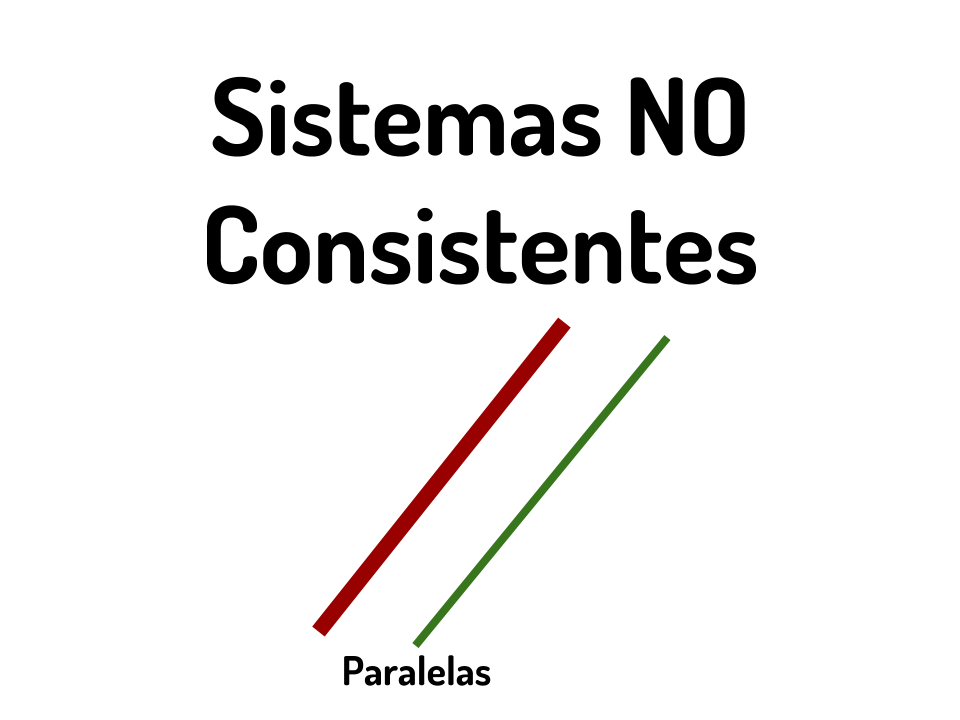
\includegraphics[width=0.60\textwidth]{SistemasNoConsistentes}
            \end{figure}


        % =====================================================
        % ========       SISTEMAS CONSISTENTES     ============
        % =====================================================
        \clearpage
        \section{Sistemas Consistentes}

            Podemos tener primeramente sistemas consistentes, es decir que tienen \textbf{mínimo}
            una solución.

            Es decir que las $n$ rectas (o lo que sea que sea el análogo en n-dimensiones)
            se interesectan MÍNIMO en un punto.

            Además algo muy interesante es que todo sistema homogéneo, osea que sus coeficientes
            independientes valgan cero es consistente. Donde la solución mas obvia es que
            todas las variables $x_i$ valgan CERO.

            \begin{figure}[h]
                \centering
                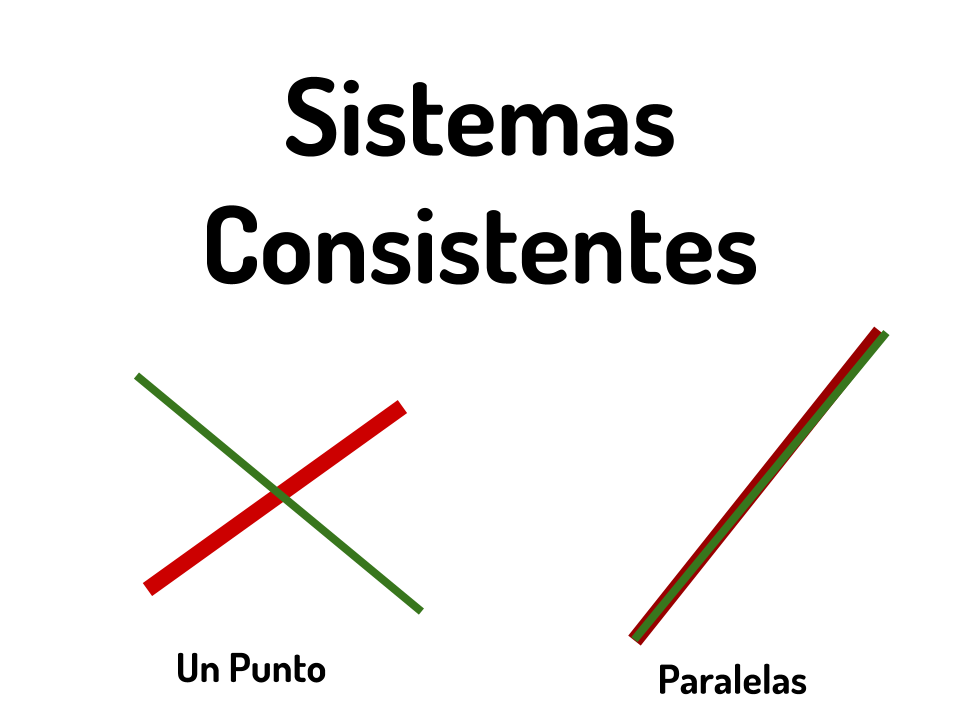
\includegraphics[width=0.60\textwidth]{SistemasConsistentes}
            \end{figure}


            % =====================================================
            % =======             PROPIEDADES              ========
            % =====================================================
            \vspace{1em}
            \subsection{Propiedades}

                \begin{itemize}
                    \item 
                        Sea $A \vec x = \vec b$ un sistema de ecuaciones lineales
                        entonces el sistema es consistente si y solo si 
                        $rango(A) = rango(A | b)$


                    \item
                        El sistema $A \vec x = \vec b$ tiene solución si y solo si $b \in R[L_A]$.

                        % ======== DEMOSTRACION ========
                        \begin{SmallIndentation}[1em]
                            \textbf{Demostración}:
                            
                            Esta es por definición, $b \in R[L_A]$ si y solo si existe un vector
                            $\vec x$ tal que $L_A(\vec x) = \vec b$ y esto ocurre si y solo si
                            $A \vec x = \vec b$.

                        \end{SmallIndentation}
                            
                \end{itemize}



            
            % =====================================================
            % =======    VARIABLES PRINCIPALES Y LIBRES    ========
            % =====================================================
            \clearpage
            \subsection{Variables Principales y Libres}

                Si una matriz aumentada de un sistema de ecuaciones
                se lleva a su forma escalonada reducida por filas
                entonces decimos que:

                \begin{itemize}
                    \item \textbf{Variables Principales:}
                        Son aquellas variables que estan relacionadas
                        con un pivote
                    \item \textbf{Variables Libres:}
                        Son aquellas variables que estan relacionadas
                        con filas llenas de ceros.
                \end{itemize}


                % ======== EJEMPLO ========
                \begin{SmallIndentation}[3em]
                    \textbf{Ejemplo}:
                    Considera esta matriz escalonada reducida por filas:
                    \begin{align*}
                        \begin{bmatrix}[c c c c c c]
                            1&0&0&0&0&0                                     \\
                            0&1&0&\frac{1}{4}&\frac{-3}{4}&\frac{-3}{4}     \\
                            0&0&1&\frac{3}{4}&\frac{-1}{4}&\frac{1}{4}      \\
                            0&0&0&0&0&0
                        \end{bmatrix}
                    \end{align*}

                    Entonces podemos ver que llegamos a estas ecuaciones:
                    \begin{align*}
                        x_1 &= 0                                                \\
                        x_2 + \frac{1}{4}x_4 - \frac{3}{4}x_5 &= -\frac{3}{4}   \\
                        x_3 + \frac{3}{4}x_4 - \frac{1}{4}x_5 &= \frac{1}{4}
                    \end{align*}

                    Por lo tanto vamos a llegar a que:
                    \begin{align*}
                        x_1 &= 0                                            \\
                        x_2 &= -\frac{1}{4}r + \frac{3}{4}s - \frac{3}{4}   \\
                        x_3 &= -\frac{3}{4}r + \frac{1}{4}s + \frac{1}{4}   \\
                        x_4 &= r                                            \\
                        x_5 &= s
                    \end{align*}  

                    Es decir llegamos a que el sistema tiene una solución
                    muy bonita para cada $r, s$, \textbf{por eso las llamamos
                    variables libres}
                
                \end{SmallIndentation}


            % =====================================================
            % =======          SISTEMAS HOMOGENEOS         ========
            % =====================================================
            \clearpage
            \subsection{Sistemas Homogeneos}
            
                Supón que tenemos el siguiente sistema $A \vec x = \vec b$, entonces decimos que el sistema
                es homogeneo si y solo si $b = 0_{m \times 1}$

                % =====================================================
                % =======             PROPIEDADES              ========
                % =====================================================
                \vspace{1em}
                \subsubsection{Propiedades}

                    \begin{itemize}
                        \item 
                            Sea $K$ el conjunto de todas las soluciones a $A \vec x = \vec 0$.

                            Entonces $K = Kernel(L_A)$, por lo tanto el conjunto de soluciones es un subespacio
                            de $\GenericField^n$ de dimensión $n - rango(L_A) = n - rango(L_A)$ donde $n$ es el 
                            número de incognitas.

                            % ======== DEMOSTRACION ========
                            \begin{SmallIndentation}[1em]
                                \textbf{Demostración}:
                                
                                Claramente podemos escribir a $K$ como $K = \Set{\vec s \in \GenericField^n \Such A \vec s = \vec 0}$.

                                La segunda parte sale inmediatamente del teorema de la dimensión.
                            
                            \end{SmallIndentation}

                        \item
                            Si es que $m < n$ entonces el sistema de $A \vec x = \vec 0$ tiene una solución no trivial

                        \item
                            Sea $K$ el conjunto de soluciones para el sistema $A \vec x = \vec b$, y sea
                            $K_H$ el conjunto de soluciones para el sistema $A \vec x = \vec 0$.

                            Entonces podemos escribir para cualquier solución $\vec s$ al conjunto de soluciones
                            como:
                            \begin{align*}
                                K = \Set{\vec s} + K_H
                                  = \Set{\vec s + \vec k \Such \vec k \in K_H}
                            \end{align*}

                            % ======== DEMOSTRACION ========
                            \begin{SmallIndentation}[1em]
                                \textbf{Demostración}:
                                
                                Suponte cualquier solución para el sistema de ecuaciones $\vec s$, tomando a otra solución $\vec w$
                                entonces $A\vec w = b$.

                                Por lo tanto:
                                \begin{align*}
                                    A (\vec w - \vec s)
                                        &= A \vec w - A \vec s      \\
                                        &= b - b                    \\
                                        &= 0
                                \end{align*}

                                Por lo tanto $\vec w - \vec s$ es solución a la ecuación homogenea por lo tanto $\vec s - \vec w \in K_H$
                                Es decir existe $\vec k \in K_H$ tal que $\vec k = \vec s - \vec w$, entonces, por lo
                                tanto $\vec w = \vec s + \vec k \in \Set{s} + K_H$.

                                Es decir $K \subseteq \Set{s} + K_H$

                                Por otro lado si $\vec w \in \Set{s} + K_H$ entonces podemos decir que $\vec w = \vec s + \vec k$,
                                pero entonces $A\vec w = A\vec s + A \vec K = \vec b + \vec 0$, por lo tanto $\vec w \in K$.

                                Por lo tanto $\Set{s} + K_H \subseteq K$

                            \end{SmallIndentation}
                                
                                

                    \end{itemize}

            % ==================================================
            % ===   SISTEMAS CONSISTENTES  INDEPENDIENTES  =====
            % ==================================================
            \clearpage
            \subsection{Sistemas Consistentes Independientes}

                Que es lo esperado y a lo que yo llamaría normal.
                Por lo tanto si tocan en un punto entonces solo habrá una única solución.

                Esto pasa si es que no hay variables libres en el sistema


                % =====================================================
                % =======             PROPIEDADES              ========
                % =====================================================
                \vspace{1em}
                \subsubsection{Propiedades}

                    \begin{itemize}
                        \item 
                            Sea $A \vec x = \vec b$ un sistema de n ecuaciones
                            con n incognitas.

                            A es invertible si y solo si el sistema tiene una
                            sola solución

                            % ======== DEMOSTRACION ========
                            \begin{SmallIndentation}[1em]
                                \textbf{Demostración}:
                                
                                Supongamos que $A$ es invertible entonces
                                $A(A^{-1}\vec b) = \vec b$, entonces $A^{-1}b$
                                es una solución.

                                Ahora, supón otra solución $\vec s$
                                entonces $A \vec s = \vec b$ al multiplicar
                                todo por la inversa tenemos que $\vec s = A^{-1}\vec b$

                                Por el otro lado si es sistema solo tiene una solución
                                entonces el conjunto de soluciones homogeneas solo
                                puede ser $\Set{\vec 0}$, por lo tanto $N(L_A) = \Set{\vec 0}$
                                entonces $A$ es invertible
                            
                            \end{SmallIndentation}
                                

                    \end{itemize}


            % ==================================================
            % ===   SISTEMAS CONSISTENTES DEPENDIENTES     =====
            % ==================================================
            \clearpage
            \subsection{Sistemas Consistentes Dependientes}

                Este caso es muy especial, pues nos dice que el sistema esta
                dado por ecuaciones que son múltiplos de la otra o otra forma
                de verlo es que esta dado por vectores linealmente dependientes.

                Podemos despejar las variables principales en términos de las variables
                libres para obtener las soluciones, así que, debido a la presencia
                de variables libres el sistema tiene infinitas soluciones.




    % ===============================================================================
    % ===================    GAUSS-JORDAN Y LOS AMIGOS         ======================
    % ===============================================================================
    \clearpage
    \chapter{Gauss-Jordan y sus Amigos}



        % ==============================================
        % =====     ELIMINACION GAUSSIANA       ========
        % ==============================================
        \clearpage
        \section{Eliminación Gaussiana}


            % ==============================================
            % =====   MATRIZ ESCALONADA POR FILAS     ======
            % ==============================================
            \subsection{Matriz Escalonada por Filas}

                Nuestro objetivo es usando las operaciones elementales encontrar una
                forma de pasar nuestra matriz ampliada a esta forma:
                \begin{align*}
                    \textcolor{Indigo700MD}{
                        \begin{bmatrix}[lll|r]
                            1 & * & * & * \\
                            0 & 1 & * & * \\
                            0 & 0 & 1 & * 
                        \end{bmatrix}
                    }
                \end{align*}

                Ok, esto no es una definición muy matemática, estas no tienen porque
                ser matrices cuadradas, pero tienen que cumplir con las siguientes
                características:
                \begin{itemize}
                    \item 
                        Para toda fila, \textbf{si} existe un elemento distinto de cero en la fila
                        \textbf{(al que llamaremos pivote)}, entonces para todos los
                        elementos anteriores  de la fila deben ser cero y este elemento
                        \textbf{(pivote) debe ser uno, la unidad}.
                    \item
                        Los pivotes deben aparecer de forma escalonada (excepto si es que la
                        fila es nula).
                    \item
                        Si una fila no tiene pivotes entonces toda esa fila debe ser nula.
                    \item
                        Si una fila no tiene pivotes (osea que sea nula) entonces todas
                        las filas de abajo no pueden tener pivotes.
                \end{itemize}

                % =========================
                % ======== EJEMPLO ========
                % =========================
                \vspace{1em}
                \begin{SmallIndentation}[1em]
                
                    \begin{ColorText}{Red700MD}
                        \textbf{Ejemplo de Cosas que NO son}:
                        \begin{align*}
                            \bVector{2&5\\6&0}
                            \MegaSpace
                            \bVector{1&4&3\\0&1&7\\0&0&8}
                            \MegaSpace
                            \bVector{1&3&2&1\\1&-1&0&0\\0&0&1&0}
                        \end{align*}
                                
                    \end{ColorText}

                    \begin{ColorText}{Green700MD}
                        \textbf{Ejemplo de Cosas que SI son}:
                        \begin{align*}
                            \bVector{1&3&4\\0&1&7\\0&0&1}
                            \MegaSpace
                            \bVector{0&1&4\\0&0&1\\0&0&0}
                            \MegaSpace
                            \bVector{0&1&4&3\\0&0&0&1\\0&0&0&0}
                        \end{align*}
                                
                    \end{ColorText}


                \end{SmallIndentation}



            % ==============================================
            % ===========       ALGORITMO     ==============
            % ==============================================
            \clearpage
            \subsection{Algoritmo}

                \begin{enumerate}
                    \item 
                        Inicias en el primer elemento, es decir $[Matriz]_{1, 1}$
                    \item 
                        Convierte ese elemento a uno (usando la operación escalar)
                    \item
                        Usas ese uno que acabas de crear (usando la operación pivot)
                        para hacer a toda a parte de abajo de la columna sea cero
                    \item
                        Te mueves a la siguiente columna y bajas un elemento el columna
                        y repites desde el paso uno.
                \end{enumerate}




        % ==============================================
        % =====     ELIMINACION GAUSSIANA       ========
        % ==============================================
        \clearpage
        \section{Gauss-Jordan}


            % ==============================================
            % =====   MATRIZ ESCALONADA POR FILAS     ======
            % ==============================================
            \subsection{Matriz Escalonada Reducida por Filas}

                Nuestro objetivo es usando las operaciones elementales encontrar una
                forma de pasar nuestra matriz ampliada a esta forma:
                \begin{align*}
                    \textcolor{Indigo700MD}{
                        \begin{bmatrix}[lll|r]
                            1 & 0 & 0 & * \\
                            0 & 1 & 0 & * \\
                            0 & 0 & 1 & * 
                        \end{bmatrix}
                    }
                \end{align*}

                Ok, esto no es una definición muy matemática, estas no tienen porque
                ser matrices cuadradas, pero tienen que cumplir con las siguientes
                características:
                \begin{itemize}
                    \item 
                        Para toda fila, \textbf{si} existe un elemento distinto de cero en la fila
                        \textbf{(al que llamaremos pivote)}, entonces para todos los
                        elementos anteriores  de la fila deben ser cero y este elemento
                        \textbf{(pivote) debe ser uno, la unidad}.
                    \item
                        Los pivotes deben aparecer de forma escalonada (excepto si es que la
                        fila es nula).
                    \item
                        Si una fila no tiene pivotes entonces toda esa fila debe ser nula
                    \item
                        Si una fila no tiene pivotes (osea que sea nula) entonces todas
                        las filas de abajo no pueden tener pivotes.


                \end{itemize}

                % =========================
                % ======== EJEMPLO ========
                % =========================
                \vspace{1em}
                \begin{SmallIndentation}[1em]

                    \begin{ColorText}{Green700MD}
                        \textbf{Ejemplo de Cosas que SI son}:
                        \begin{align*}
                            \bVector{1&0&0\\0&1&0\\0&0&1}
                            \MegaSpace
                            \bVector{1&0&0&0\\0&0&1&0\\0&0&0&1}
                            \MegaSpace
                            \bVector{1&7&0&1&0\\0&0&1&4&0\\0&0&0&0&1\\0&0&0&0&0}
                        \end{align*}
                                
                    \end{ColorText}


                \end{SmallIndentation}



            % ==============================================
            % ===========       EJEMPLOS      ==============
            % ==============================================
            \clearpage
            \subsection{Ejemplos}
    
            \begin{SmallIndentation}[1em]
                
                % ======== EJEMPLO ========
                \textbf{Ejemplo 1}:
                    
                    Nota este sistema de ecuaciones:
                    \begin{MultiLineEquation*}{3}
                        2x_1 &-  x_2 &+ 4x_3 &= -3       \\
                         x_1 &+ 2x_2 &- 3x_3 &= 1        \\
                        5x_1 &+ 3x_2 &+  x_3 &= -2  
                    \end{MultiLineEquation*}

                    Ahora, ve esto:
                    \begin{align*}
                        \begin{bmatrix}[r r r | r]
                            2 & -1 &  4 & -3       \\
                            1 &  2 & -3 &  1       \\
                            5 &  3 &  1 & -2  
                        \end{bmatrix}
                    \end{align*}

                    Ahora, apliquemos Gauss-Jordan:
                    \begin{align*}
                        &
                        \begin{bmatrix}[r r r | r]
                            2 & -1 &  4 & -3       \\
                            1 &  2 & -3 &  1       \\
                            5 &  3 &  1 & -2  
                        \end{bmatrix}
                        &&
                        \overset{F_1 \lEqual F_2}{\lLongTo}
                        &&
                        \begin{bmatrix}[r r r | r]
                            1 &  2 & -3 &  1       \\
                            2 & -1 &  4 & -3       \\
                            5 &  3 &  1 & -2  
                        \end{bmatrix}
                        &&
                        \overset{F_2 = F_2 -2F_1}{\lLongTo}
                        &&
                        \begin{bmatrix}[r r r | r]
                            1 &  2 & -3 &  1       \\
                            0 & -5 & 10 & -5       \\
                            5 &  3 &  1 & -2  
                        \end{bmatrix}
                        \\
                        &
                        \begin{bmatrix}[r r r | r]
                            1 &  2 & -3 &  1       \\
                            0 & -5 & 10 & -5       \\
                            5 &  3 &  1 & -2  
                        \end{bmatrix}
                        &&
                        \overset{F_3 = F_3 -5F_1}{\lLongTo}
                        &&
                        \begin{bmatrix}[r r r | r]
                            1 &  2 & -3  &  1       \\
                            0 & -5 & 10  & -5       \\
                            0 & -7 & 16  & -7  
                        \end{bmatrix}
                        &&
                        \overset{F_2 = -\frac{1}{5}F_2}{\lLongTo}
                        &&
                        \begin{bmatrix}[r r r | r]
                            1 &  2 & -3  &  1       \\
                            0 & 1  & -2  & 1        \\
                            0 & -7 & 16  & -7  
                        \end{bmatrix}
                        \\
                        &
                        \begin{bmatrix}[r r r | r]
                            1 &  2 & -3  &  1       \\
                            0 & 1  & -2  & 1        \\
                            0 & -7 & 16  & -7  
                        \end{bmatrix}
                        &&
                        \overset{F_1 = F_1 -2F_2}{\lLongTo}
                        &&
                        \begin{bmatrix}[r r r | r]
                            1 & 0  & 1   & -1       \\
                            0 & 1  & -2  &  1       \\
                            0 & -7 & 16  & -7  
                        \end{bmatrix}
                        &&
                        \overset{F_1 = F_1 -2F_2}{\lLongTo}
                        &&
                        \begin{bmatrix}[r r r | r]
                            1 & 0  & 1   & -1       \\
                            0 & 1  & -2  &  1       \\
                            0 & -7 & 16  & -7  
                        \end{bmatrix}
                        \\
                        &
                        \begin{bmatrix}[r r r | r]
                            1 & 0  & 1   & -1       \\
                            0 & 1  & -2  &  1       \\
                            0 & -7 & 16  & -7  
                        \end{bmatrix}
                        &&
                        \overset{F_3 = F_3 + 7F_2}{\lLongTo}
                        &&
                        \begin{bmatrix}[r r r | r]
                            1 & 0  & 1   & -1       \\
                            0 & 1  & -2  &  1       \\
                            0 & 0  &  2  & 0  
                        \end{bmatrix}
                        &&
                        \overset{F_3 = \frac{1}{2}F_3}{\lLongTo}
                        &&
                        \begin{bmatrix}[r r r | r]
                            1 & 0  &  1  & -1       \\
                            0 & 1  & -2  &  1       \\
                            0 & 0  &  1  &  0  
                        \end{bmatrix}
                        \\
                        &
                        \begin{bmatrix}[r r r | r]
                            1 & 0  &  1  & -1       \\
                            0 & 1  & -2  &  1       \\
                            0 & 0  &  1  &  0  
                        \end{bmatrix}
                        &&
                        \overset{F_1 = F_1 - F_3}{\lLongTo}
                        &&
                        \begin{bmatrix}[r r r | r]
                            1 & 0  &  0  & -1       \\
                            0 & 1  & -2  &  1       \\
                            0 & 0  &  1  &  0  
                        \end{bmatrix}
                        &&
                        \overset{F_2 = F_2 + 2F_3}{\lLongTo}
                        &&
                        \begin{bmatrix}[r r r | r]
                            1 & 0  &  0  & -1       \\
                            0 & 1  &  0  &  1       \\
                            0 & 0  &  1  &  0  
                        \end{bmatrix}
                    \end{align*}

                    Ahora si, creo que ahora es más que obvio que:
                    \begin{align*}
                        x_1 &= -1   \\
                        x_2 &=  1   \\
                        x_3 &=  0
                    \end{align*}

            \end{SmallIndentation}
                



        % ==============================================
        % ====        INVERSA DE UNA MATRIZ       ======
        % ==============================================
        \clearpage
        \section{Inversa de una Matriz}

            Sea $A \in M_{n \times n}(\GenericField)$ y entonces definimos a $A^{-1}$ 
            de forma informal como aquella matriz que cumple con que $A^{-1}A = AA^{-1} = I_{n}$
            nota que no para todas las matrices $M_{n \times n}(\GenericField)$ existe una matriz inversa.


           \subsubsection*{El Problema de la Notación $A^{-1}$}

           El problema con esta notación es que existen matrices no invertibles, para las cuales
           la notación $A^{-1}$ no tiene sentido.

           La notación $A^{-1}$ se puede usar solamente despúes de demostrar que $A$ es invertible.

            % ===============================
            % =========   PROPIEDADES =======
            % ===============================
            \clearpage
            \subsection{Propiedades}

                \begin{itemize}

                    \item La Matriz Inversa de $A$ ($A^{-1}$) es única.

                        % ======== DEMOSTRACION ========
                        \begin{SmallIndentation}[1em]
                            \textbf{Demostración}:

                            Lo que hay que ver que si $A,B,C \in M_n(\GenericField)$ tales que
                            $AB = BA = I_n$ y $AC = CA = I_n$. Entonces $B=C$.

                            Usando la Ley asociativa de la Multiplicación de Matrices $(A(BC)=(AB)C)$
                            tenemos que:
                            $B = B(I_n) = B(AC) = (BA)C = I_nC =  C $

                        \end{SmallIndentation}

                    \item Es necesario aunque no suficiente que todas las columnas y filas de una
                        matriz $A \in M_{n \times n}$ sea diferentes de cero para que $A$ sea invertible.

                        % ======== DEMOSTRACION ========
                        \begin{SmallIndentation}[1em]
                            \textbf{Demostración}:

                            Renglones Nulos:

                                Sea $A \in M_{n \times n}(\GenericField)$.
                                Supongamos que (por lo menos) un renglón de A es nulo, es decir:
                                $[A]_{p,*} = 0_{1,n}$ donde $0 < p \leq n$ esto es lo mismo que decir
                                que $\forall j \in \{1, \dots, n\} [A]_{p,j} = 0$.

                                Ahora supongamos que $A$ es invertible, entonces, en particular, la entrada
                                $(p,p)$ del producto $AA^{-1}$ debe coincidir con la entrada $(p,p)$ de la
                                matriz identidad $I_n$.
                                Podemos calcular esa entrada como
                                $[AA^{-1}]_{p,p} = \sum_{k=1}^{n} [A]_{p,k} [A^{-1}]_{k,p}$
                                esto debería ser $[I_n]_{p,p}=1$ pero ya vimos que $[A]_{p,k} = 0$, es decir
                                $0 = 1$. Contradicción.


                            Columnas Nulas:
                                Sea $A \in M_{n \times n}(\GenericField)$.
                                Supongamos que (por lo menos) una columna de A es nulo, es decir:
                                $[A]_{*,p} = 0_{n,1}$ donde $0 < p \leq n$ esto es lo mismo que decir
                                que $\forall j \in \{1, \dots, n\} [A]_{p,j} = 0$.

                                Ahora supongamos que $A$ es invertible, entonces, en particular, la entrada
                                $(p,p)$ del producto $A^{-1}A$ debe coincidir con la entrada $(p,p)$ de la
                                matriz identidad $I_n$.

                                Podemos calcular esa entrada como
                                $[A^{-1}A]_{p,p} = \sum_{k=1}^{n} [A^{-1}]_{p,k} [A]_{k,p}$
                                esto debería ser $[I_n]_{p,p}=1$ pero ya vimos que $[A]_{k,p} = 0$, es decir
                                $0 = 1$. Contradicción.
                            
                        \end{SmallIndentation}

                    \item Sea $A,B \in M_{m \times n}(\GenericField)$ y sean invertibles, entonces tenemos
                        que $(AB)^{-1} = B^{-1}A^{-1}$

                        % ======== DEMOSTRACION ========
                        \begin{SmallIndentation}[1em]
                            \textbf{Demostración}:

                            Si $(AB)$ es invertible entonces tenemos que probar que:
                            \begin{align*}
                                (AB)(B^{-1}A^{-1})  &=                      \\
                                                    &= (((AB)B^{-1})A^{-1})  
                                                    &= ((A(BB^{-1}))A^{-1}) 
                                                    &= ((A(I_n))A^{-1})     
                                                    &= (AA^{-1})            \\
                                                    &= I_n 
                            \end{align*}
                            
                        \end{SmallIndentation}

                    \clearpage

                    \item Una Matriz Diagonal es invertible si y solo si los elementos de la diagonal
                        son distintos de cero.

                    \item Una Matriz Diagonal es invertible si y solo si los elementos de la diagonal
                        son distintos de cero.

                    \item Sea $A \in M_{m \times n}(\GenericField)$ y sea invertible, entonces tenemos
                        que $(A^{-1})^{-1} = A$

                    \item Sea $A \in M_{m \times n}(\GenericField)$ y sea invertible, entonces tenemos
                        que $(A^T)^{-1} = (A^{-1})^T$

                    \item
                        Sea $A \in M_{n \times n}(\GenericField)$ tal que $A$ sea invertible y triangular superior, 
                        entonces $A^{-1}$ es triangular también.

                        % ======== DEMOSTRACION ========
                        \begin{SmallIndentation}[1em]
                            \textbf{Demostración}:
                            
                            Ok, para esta demostración nos vamos a apoyar en otras propiedades.

                            Por un lado, sabemos que $A$ es invertible, es decir podemos realizar una serie finita de operaciones
                            elementales que transforman a $A$ en la identidad, ahora, lo interesante es que esas operaciones elementales
                            son triangulares (2 de ellas, la del escalar e sumar a una fila superior un multiplo de una fila inferior,
                            pero con esas 2 nos basta).

                            Y que el producto de matrices triangulares es también otra matriz triangular, por lo tanto si $A$ es triangular
                            entonces $A^{-1}$ también es triangular.
                        
                        \end{SmallIndentation}
                            

                \end{itemize}
            




% //////////////////////////////////////////////////////////////////////////////////////////////////////////
% /////////////////////////////              DETERMINANTES               ///////////////////////////////////
% //////////////////////////////////////////////////////////////////////////////////////////////////////////
\part{Determinantes}
\clearpage


    % ===============================================================================
    % ===================            INTRODUCCION                 ===================
    % ===============================================================================
    \chapter{Determinantes de $2 \times 2$}


        % ==============================================
        % ========          DEFINICION           =======
        % ==============================================
        \clearpage
        \section{Definición}

            La idea es construir recursivamente el concepto, por lo
            cual comenzaremos por construir los determinantes de $2 \times 2$

            Sea $A \in M_{2 \times 2}(\GenericField)$ definida como:
            \begin{align*}
                A = \pVector{a_{11} & a_{12} \\ a_{21} & a_{22}}
            \end{align*}

            Entonces definimos al determinante como:
            \begin{align*}
                |A| := a_{11} a_{22} - a_{12} a_{21} 
            \end{align*}

            Claramente el $det(A) \in \GenericField$ y es importante
            recordar que $det(A)$ \textbf{no es una transformación lineal}

            Otra cosa importante que recordar es que en el siguiente capitulo veremos
            que esto no es una definición simplemente una consecuencia de la definición
            formal de un determinante.




        % ==============================================
        % ========        PROPIEDADES            =======
        % ==============================================
        \clearpage
        \section{Propiedades}

            \begin{itemize}

                \item
                    $det(A) = det(A^T)$

                    % ======== DEMOSTRACION ========
                    \begin{SmallIndentation}[1em]
                        \textbf{Demostración}:
                        
                        Ya sabemos cual es el determinate ahora, simplemente
                        tenemos que sacar el:
                        \begin{align*}
                            det\Wrap{A^T}
                                &= det\Wrap{\pVector{a_{11} & a_{12} \\ a_{21} & a_{22}}^T}     \\
                                &= det\Wrap{\pVector{a_{11} & a_{21} \\ a_{12} & a_{22}}}       \\
                                &= a_{11} a_{22} - a_{21} a_{12}
                        \end{align*}
                    
                    \end{SmallIndentation}
                        

                \item 
                    La función del determinante es una función lineal
                    para cada renglón, dejando fijo al otro

                    Es decir dados $\vec u, \vec v, \vec w \in \GenericField^2$ y
                    y $k \in \GenericField$ entonces:
                    \begin{align*}
                        det \pVector{\vec u + k\vec v \\ \vec w}
                            =  det \pVector{\vec u \\ \vec w}
                            + det k\pVector{\vec v \\ \vec w}
                    \end{align*}

                    Y 
                    \begin{align*}
                        det \pVector{\vec w \\ \vec u + k\vec v}
                            =  det \pVector{\vec w  \\ \vec u}
                            + det k\pVector{\vec w  \\ \vec v}
                    \end{align*}


                    % ======== DEMOSTRACION ========
                    \begin{SmallIndentation}[1em]
                        \textbf{Demostración}:
                        
                        Es pura talacha men :v
                        
                    
                    \end{SmallIndentation}

                \item
                    $det(A) \neq 0$ si y solo si $A$ es invertible

                    % ======== DEMOSTRACION ========
                    \begin{SmallIndentation}[1em]
                        \textbf{Idea de la Demostración}:
                        
                        Podemos ver que la inversa de $A$ esta dada
                        por:
                        \begin{align*}
                            A^{-1}
                                = \frac{1}{det(A)} \pVector{
                                                         a_{22} & -a_{12} \\
                                                        -a_{21} &  a_{11}
                                                    }
                        \end{align*}

                        Podemos ver claramente que funciona como la inversa, pero
                        necesita que $det(A)$ no sea cero para que tenga sentido, ese
                        es el sentido de la demostración
                    
                    \end{SmallIndentation}


                \item
                    Si $A \in M_{2 \times 2}(\GenericField)$ y $A$ tiene dos filas iguales
                    entonces su determinante es cero

                \item
                    $det(Id_{2 \times 2}) = 1$

                \clearpage

                \item
                    Sea $\delta: M_{2 \times 2}(\GenericField) \to \GenericField$ una función
                    tal que:
                    \begin{itemize}
                        \item $\delta$ es lineal por renglones
                        \item Si la matriz $A$ tiene renglones o filas iguales entonces tenemos que
                            $\delta(A) = 1$
                        \item $\delta(Id_{2 \times 2}) = 1$
                    \end{itemize}

                    Entonces $\delta = det$

                \item
                    La combinación lineal de funciones n-lineales es n-lineal

                \item
                    Si $\delta$ es una función alternante, entonces si es que
                    para 2 matrices $A, B$ tal que $B$ es igual a $A$ excepto
                    porque tienen las filas $i, j$ cambiadas entonces
                    $\delta(A) = - \delta(B)$.

            \end{itemize}







    % ===============================================================================
    % ============      DETERMINANTES EN GENERAL                  ===================
    % ===============================================================================
    \chapter{Determinantes en General}

        % ==============================================
        % ========          NOTACION             =======
        % ==============================================
        \clearpage
        \section{Notación}

            Dada $A \in M_{n \times n}(\GenericField)$ entonces decimos que
            $\tilde A_{i, j} \in M_{n-1 \times n-1}(\GenericField)$ es la matriz $A$
            pero sin la fila $i$ ni la columna $j$.

            % ======== EJEMPLO ========
            \begin{SmallIndentation}[1em]
                \textbf{Ejemplo}:
                
                Por ejemplo $A = \pVector{
                    1 & 2 & 3   \\
                    4 & 5 & 6   \\
                    7 & 8 & 9   \\
                }$ entonces $\tilde A_{1, 1} = \pVector{
                    5 & 6   \\
                    8 & 9   \\
                }$ entonces $\tilde A_{3, 2} = \pVector{
                    1 & 3   \\
                    4 & 6   \\
                }$ 
            
            \end{SmallIndentation}
                


        % ==============================================
        % ======     DEFINICION RECURSIVA        =======
        % ==============================================
        \vspace{1em}
        \section{Definición Recursiva}

            Sea $A \in M_{n \times n}(\GenericField)$ entonces tenemos que:
            \begin{align*}
                det(A) := \sum_{i = 1}^n (-1)^{x + i} [A]_{x, i} \; det(\tilde A_{x, i})
            \end{align*}

            Esta función funciona para cualquier $x \in [1, \dots, n]$

            Bajo esta definición es importante denotar que el escalar 
            $(-1)^{1 + i} [A]_{i, j} det(\tilde A_{i, j})$ es llamado cofactor.



        % ==============================================
        % ====    CARACTERISTICAS IMPORTANTES     ======
        % ==============================================
        \clearpage
        \section{Características Importantes}


            % ==============================================
            % ========          N-LINEAL             =======
            % ==============================================
            \subsection{N-Lineal}

                Decimos que una función es $n-lineal$ si es que para una matriz de $m \times n$
                (Recuerda que $[A]^i$ es la i-ésima fila horizontal de la matriz):
                \begin{align*}
                    \delta\pVector{\Brackets{A}^1 \\ \vdots \\ c\Brackets{A}^i + \Brackets{A}^j \\ \vdots \\ \Brackets{A}^m}
                        &= c
                        \delta\pVector{\Brackets{A}^1 \\ \vdots \\ \Brackets{A}^i \\ \vdots \\ \Brackets{A}^m}
                        + \delta\pVector{\Brackets{A}^1 \\ \vdots \\ \Brackets{A}^j \\ \vdots \\ \Brackets{A}^m}
                \end{align*}


            % ==============================================
            % ========         ALTERNANTE            =======
            % ==============================================
            \vspace{1em}
            \subsection{Alternante}

                Decimos que una función $\delta$ es alternante si y solo si $\delta(A) = 0$
                si es que $[A]^i = [A]^j$ (es decir si es que 2 columnas son iguales)




        % ==============================================
        % ========          DEFINICION           =======
        % ==============================================
        \vspace{1em}
        \section{Definición por Propiedades}

            Un determinante es una función que va del espacio de las matrices cuadradas
            a el campo, es una función que:
            \begin{itemize}
                \item Es n-lineal
                \item Es alternante
                \item Evaluada en cualquier identidad nos da el uno del campo
            \end{itemize}




            % ==============================================
            % ========        PROPIEDADES            =======
            % ==============================================
            \clearpage
            \subsection{Propiedades}

                \begin{itemize}

                    \item
                        $det(A) \neq 0$ si y solo si $A$ es invertible

                    \item
                        Si $A \in M_{n \times n}(\GenericField)$ tiene un rango menor que $n$
                        entonces $det(A) = 0$

                    \item
                        Si $A \in M_{n \times n}(\GenericField)$ tiene 2 columnas o filas iguales entoces
                        $det(A) = 0$

                    \item
                        Si $A \in M_{n \times n}(\GenericField)$ y $A$ tiene dos filas iguales
                        entonces su determinante es cero

                    \item
                        Si $A \in M_{n \times n}(\GenericField)$ y $B$ es igual a $A$ pero con una
                        columna cambiada entonces $det(A) = - det(B)$

                    \item
                        Si $A \in M_{n \times n}(\GenericField)$ y $B$ es igual a $A$ pero se sumo un
                        multiplo de una fila de $A$ a otra fila de $A$.

                        Entonces $det(A) = det(B)$

                    \item
                        
                        Si $A \in M_{n \times n}(\GenericField)$ entonces $det(cA) = c^n \; det(A) \forall c \in \GenericField$
                        % ======== DEMOSTRACION ========
                        \begin{SmallIndentation}[1em]
                            \textbf{Demostración}:
                            
                            Recuerda que por definición el determinante es una función $n-lineal$, entonces
                            podemos ver al determinante de $A$ como:
                            \begin{align*}
                                det\Wrap{cA}
                                    = det\pVector{ca_1 \\ ca_2 \\ \ldots  \\ca_n }              
                                    = c \; det\pVector{a_1 \\ ca_2 \\ \ldots  \\ca_n }          
                                    = c^2 \; det\pVector{a_1 \\ a_2 \\ \ldots  \\ca_n } 
                                    = \dots        
                                    = c^n \; det\pVector{a_1 \\ a_2 \\ \ldots  \\ a_n }
                            \end{align*}
                        
                        \end{SmallIndentation}


                    \item
                        Sea $\beta = \Set{\vec x_1, \dots \vec x_n}$ donde cada uno $\vec x_i \in \GenericField^n$
                        y si tenemos $A \in M_{n \times n}(\GenericField)$ y $A_i = \vec x_i$.

                        Entonces si $\beta$ es una base de $\GenericField^n$ entonces $det(B) \neq 0$.

                        % ======== DEMOSTRACION ========
                         \begin{SmallIndentation}[1em]
                             \textbf{Demostración}:
                             
                            Es decir, podemos reescribirlo como que si $\beta$ NO es una base de $\GenericField^n$
                            entonces $det(B) = 0$.

                            Sabemos que si $\beta$ no es base, entonces no es linealmente independiente es decir
                            que existe algún vector dentro de $\beta$ que podemos obtener de la combinación lineal
                            de los otros. Es decir que el rango de la matriz no es $n$, y ya habiamos visto que matrices
                            con un rango menor que n tiene un determinate igual a 0.

                            Ahora por otro lado si es que el determinante es cero entonces podemos asegurar que no
                            es invertible, por lo tanto su rango no es n por lo tanto no son linealmente independientes
                            sus vectores columna, por lo tanto $\beta$ no puede ser base.

                         \end{SmallIndentation}

                    \clearpage

                    \item
                        Sea $A \in M_{n \times n}(\GenericField)$ que puede ser escribirse de la forma:
                        \begin{align*}
                            A = \pVector{B_1 & B_2 \\ 0 & B_3}
                        \end{align*}

                        Donde $B_1, B_3$ son matrices cuadradas entonces $det(A) = det(B_1) \; det(B_3)$

                        % ======== DEMOSTRACION ========
                        \begin{SmallIndentation}[1em]
                            \textbf{Demostración}:

                            Para hacerlo nos vamos a basar de la afirmación que si $A = \pVector{B_1 & B_2 \\ 0 & Id}$ entonces
                            $A = det(B_1)$, esto ya no demostramos pero aún así la idea es simplemente una doble inducción primero
                            una inducción expandiendo la $n-aba$ fila y luego la $n-1$aba fial recursivamente.

                            Ahora si... vamos
                            
                            Primero si $B_3$ no es invertible entonces el conjunto de vectores fila de $B_3$
                            no es independiente, esto quiere decir que $(0 \;\; B_3)$ tampoco puede ser linealmente
                            independiente, por lo tanto es imposible que $A$ tenga un conjunto de vectores
                            fila linealmente independiente.

                            Por lo tanto $det(A) = 0 = det(B_3) = det(B_3) det(B_1)$

                            Ahora, si $B_3$ es invertible entonces tenemos esto bien bonito:
                            \begin{align*}
                                \pVector{Id & 0 \\ 0 & B_3^{-1}} \pVector{B_1 & B_2 \\ 0 & B_3} = \pVector{B_1 & B_2 \\ 0 & I}
                            \end{align*}

                            Por lo tanto obtenemos la identidad:
                            $det(B_3^{-1}) det(A) = det(B_1)$, y ya que sabemos que $det(B_3^{-1}) = det(B_3)^{-1}$ por lo tanto
                            $det(A) = det(B_1) det(B_3)$
                        
                        \end{SmallIndentation}

                \end{itemize}


        % ==============================================
        % ==   DETERMINANTES Y OPERACION ELEMENTAL  ====
        % ==============================================
        \clearpage
        \section{Determinantes y Elementales}

            \begin{itemize}
                
                \item 
                    Sea $E_{\text{Tipo 1}}$ una matriz elemental obtenida de intercambiar
                    cualquier 2 filas de la identidad, entonces $det(E) = -1$

                \item 
                    Sea $E_{\text{Tipo 2}}$ una matriz elemental obtenida de mutiplicar
                    una fila por un escalar ($k$) no cero, entonces $det(E) = k$

                \item 
                    Sea $E_{\text{Tipo 3}}$ una matriz elemental obtenida de sumar
                    un múltiplo de una fila a otra fila, entonces $det(E) = 1$

            \end{itemize}


            % ==============================================
            % ========        PROPIEDADES            =======
            % ==============================================
            \clearpage
            \subsection{Propiedades}

                \begin{itemize}

                    \item
                        Para cualquier $A, B \in M_{n \times n}(\GenericField)$
                        entonces $det(AB) = det(A) det(B)$.

                    \item
                        Si $A$ es invertible entonces $det(A^{-1}) = \dfrac{1}{det(A)}$

                    \item
                        Si $E \in M_{n \times n}(\GenericField)$ es una matriz elemental
                        entonces $det(E) = det(E^T)$

                        % ======== DEMOSTRACION ========
                        \begin{SmallIndentation}[1em]
                            \textbf{Demostración}:
                            
                            Vamos a hacerlo por partes:
                            \begin{itemize}
                                
                                \item 
                                    Si $E$ es de tipo 1 (cambio de filas o columnas) entonces
                                    sabemos que $E$ es simétrico, por lo tanto $det(E^T) = det(E)$.

                                \item 
                                    Si $E$ es de tipo 2 entonces sabemos que $E$ es simétrico,
                                    por lo tanto $det(E^T) = det(E)$.

                                \item
                                    Si es que $E$ es de tipo 3, entonces $E^T$ es también una matriz 
                                    de tipo 3, y sabemos que $det(E) = 1$ entonces $det(E^T) = 1$, por lo
                                    tanto son iguales 
                            \end{itemize}
                        
                        \end{SmallIndentation}
                            

                    \item
                        Sea $A \in M_{n \times n}(\GenericField)$
                        entonces $det(A^T) = det(A)$

                    \item
                        Sea $A \in M_{n \times n}(\GenericField)$ donde $A$ es una matriz triangular
                        superior (o inferior) es el producto de las entradas de la diagonal.

                        % ======== DEMOSTRACION ========
                        \begin{SmallIndentation}[1em]
                            \textbf{Demostración}:
                            
                            Vamos a hacer inducción sobre $n$, el tamaño de la diagonal, para una matriz de $2 \times 2$
                            creo que es más que obvio que se cumple, pues:
                            \begin{align*}
                                |A| = \Mag{\pVector{a_{11} & a_{12} \\ 0 & a_{22}}} = a_{11}a_{22} - 0a_{12} = a_{11}a_{22}
                            \end{align*}

                            Ahora considera que se cumple para una $n = k$, entonces considera una matriz de $k+1 \times k+1$
                            que sea triangular superior, entonces podemos encontrar su determinante como:
                            \begin{align*}
                                det(A) = \sum_{x = 1}^{k+1} (-1)^{x + 1} [A]_{1, x} det(\tilde A _{1, j})     
                            \end{align*} 

                            Ahora para $\tilde [A]_{1, 2}, \tilde [A]_{1, 3}, \dots \tilde A_{1, n +1}$ tiene la primera
                            columan de puros 0, por lo tanto su determinante es cero, por lo tanto esa suma inicial sobre $x$
                            se reduce a solo el primer termino.
                            \begin{align*}
                                det(A) 
                                    &= [A]_{1, 1} det(\tilde A _{1, 1})
                                        && \Remember{Mira que bonito}                       \\
                                    &= [A]_{1, 1} [A]_{2, 2} [A]_{3, 3} \dots [A]_{n+1, n+1}
                                        && \Remember{Por inducción}
                            \end{align*}

                            Ahora, sabemos que $det(A^T) = det(A)$, por lo tanto ya esta demostrado para matrices
                            triangulares inferiores.

                        \end{SmallIndentation}

                    \clearpage


                    \item
                        Sea $A \in M_{n \times n}(\GenericField)$ donde $A$ es una matriz triangular
                        superior (o inferior) entonces $A$ es invertible si y solo si en la diagonal no hay ceros

                        % ======== DEMOSTRACION ========
                        \begin{SmallIndentation}[1em]
                            \textbf{Demostración}:

                            Vamos a demostrar este enunciado pero de otra forma: Sea $A$ una matriz triangular
                            superior (o inferior) entonces A NO es invertible si y solo si en la diagonal hay ceros
                            
                            Ahora, suponte que en la diagonal hay 1 cero, entonces ya sabemos que 
                            $det(A) = \prod_{i = 1}^n [A]_{i, i}$ ahora, si hay un cero por ahí entonces
                            $det(A) = 0$, por lo tanto no puede ser invertible.

                            De modo parecido, si $A$ no es invertible entonces $det(A) \neq 0$, por lo tanto
                            tenemos que alguna de los elementos de la diagonal tiene que ser cero, pues estamos hablando
                            de elementos de un campo, en el que el producto de elementos nos da cero si y solo si alguno de 
                            ellos es cero.

                        \end{SmallIndentation}

                    \item
                        Sea $A, B \in M_{n \times n}(\GenericField)$ matrices similares entonces tenemos
                        $det(A) = det(B)$

                \end{itemize}



        % ==============================================
        % ========          COFACTOR             =======
        % ==============================================
        \clearpage
        \section{Cofactor}

            Por venir :v



        % ==============================================
        % ========          ADJUNTA A            =======
        % ==============================================
        \clearpage
        \section{Adjunta}

            Vamos a definir a la adjunta de una matriz $A \in M_{n \times n}(\GenericField)$
            como:
            \begin{align*}
                adj(A) := C^T \Space \text{donde $C$ es la matriz de cofactores}     
            \end{align*} 

            Otra manera de verla es que $\BigBrackets{adj(A)}_{i, j} = c_{j, i}$


            % ==============================================
            % ========        PROPIEDADES            =======
            % ==============================================
            \vspace{1em}
            \subsection{Propiedades}

                \begin{itemize}

                    \item
                        $adj(A^T) = adj(A)^T$

                        % ======== DEMOSTRACION ========
                        \begin{SmallIndentation}[1em]
                            \textbf{Demostración}:
                            
                            Esta debería salir por definición:
                            \begin{align*}
                                adj(A^T)
                                    &= C'^T
                                        && \Remember{Recuerda que $[C']_{i, j} = [C]_{j, i}$ }   \\
                                    &= (C'^T)^T                                            
                                        && \Remember{Por eso $C'^T = C$ }   \\
                                    &= adj(A)^T
                                        && \Remember{Magia}
                            \end{align*}
                        
                        \end{SmallIndentation}
                            

                    \item
                        Sea $A \in M_{n \times n}(\GenericField)$ entonces
                        $A^{-1} = \dfrac{1}{det(A)} \; adj(A)$

                        % ======== DEMOSTRACION ========
                        \begin{SmallIndentation}[1em]
                            \textbf{Demostración}:
                            
                            Considera primero el producto:
                            \begin{align*}
                                \bigBrackets{A \; adj(A)}_{i, j}
                                    &= \sum_{k = 1}^n 
                                        [A]_{i, k} \; [adj(A)]_{k, j}       
                                        && \Remember{Por definición de multiplicación}  \\
                                    &= \sum_{k = 1}^n 
                                        a_{i, k} \; [C^T]_{k, j}       
                                        && \Remember{Por definición de adjunta}         \\
                                    &= \sum_{k = 1}^n 
                                        a_{i, k} \; c_{j, k}       
                                        && \Remember{Otra definición de determinante}   \\
                                    &= det(A) \; \delta(i, j)                           \\
                                    &= det(A) [Id]_{i, j}                               \\
                            \end{align*}

                            Ahora como $A$ es invertible entonces podemos dividir por
                            $det(A)$, después de todo, es solo un número del campo
                            que no es cero.

                            Con esto llegamos a que:
                            $\bigBrackets{A \; \frac{adj(A)}{det(A)} }_{i, j} = [Id]_{i, j}$,
                            es decir 
                            $[A]_{i, j} \Brackets{ \frac{adj(A)}{det(A)} }_{i, j} = [Id]_{i, j}$
                            por lo tanto $\frac{adj(A)}{det(A)}$ se comporta perfectamente como
                            una inversa.
                        
                        \end{SmallIndentation}

                    \item
                        Sea $A \in M_{n \times n}(\GenericField)$ entonces
                        $det( adj(A) ) = det(A)^{n-1}$

                        % ======== DEMOSTRACION ========
                        \begin{SmallIndentation}[1em]
                            \textbf{Demostración}:
                            
                            Con la propiedad anterior ya tenemos las herramientas
                            necesarias:

                            Primero tenemos que $A^{-1} = \dfrac{adj(A)}{det(A)}$
                            entonces podemos decir que $A^{-1} det(A) = adj(A)$

                            Ahora si multiplicamos todo por $A$ tenemos que:
                            $det(A) Id = A adj(A)$, ahora si tomamos el determinante
                            de ambos lados tenemos que:
                            $det(det(A) Id) = det(A \; adj(A))$

                            Ahora del lado derecho todo tiene sentido pues
                            $det(det(A) Id) = det(A) \; det(adj(A))$.

                            Ahora lo importante es el lado izquierdo vamos a aplicar
                            la siguiente propiedad $det(cA) = c^n det(A)$, por lo tanto
                            tendremos que:

                            $det(A)^n \; (1) = det(A) \; det(adj(A))$, ahora solo despejas
                            y tienes que $det(A)^{n-1} = det(adj(A))$
                        
                        \end{SmallIndentation}

                    \item
                        Sea $A \in M_{n \times n}(\GenericField)$ tal que $A$ sea invertible y triangular superior, 
                        entonces $adj(A)$ es triangular también.

                        % ======== DEMOSTRACION ========
                        \begin{SmallIndentation}[1em]
                            \textbf{Demostración}:
                            
                            Ya sabemos que si $A$ es triangular superior, entonces $A^{-1}$ es triangular superior, ahora
                            también sabemos que $A^{-1} = \dfrac{1}{det(A)} \; adj(A)$, por lo tanto
                            la única diferencia entre $A^{-1}$ y $adj(A)$ es solo una constante, por lo tanto
                            como $A^{-1}$ es triangular superior, entonces $adj(A)$ también es triangular superior.
                        
                        \end{SmallIndentation}
                            
                            
                \end{itemize}





% ===============================================
% ========        BIBLIO      ===================
% ===============================================
\begin{thebibliography}{10}

    \bibitem{Friedberg-LinealAlgebra} 
        Friedberg,
        \textit{LinealAlgebra}. 

\end{thebibliography}







\end{document}